%%%%%%%%%%%%%%
%% Run LaTeX on this file several times to get Table of Contents,
%% cross-references, and citations.

%% If you have font problems, you may edit the w-bookps.sty file
%% to customize the font names to match those on your system.

%% w-bksamp.tex. Current Version: Feb 16, 2012
%%%%%%%%%%%%%%%%%%%%%%%%%%%%%%%%%%%%%%%%%%%%%%%%%%%%%%%%%%%%%%%%
%
%  Sample file for
%  Wiley Book Style, Design No.: SD 001B, 7x10
%  Wiley Book Style, Design No.: SD 004B, 6x9
%
%
%  Prepared by Amy Hendrickson, TeXnology Inc.
%  http://www.texnology.com
%%%%%%%%%%%%%%%%%%%%%%%%%%%%%%%%%%%%%%%%%%%%%%%%%%%%%%%%%%%%%%%%

%%%%%%%%%%%%%
% 7x10
%\documentclass{wileySev}

% 6x9
\documentclass{wileySix}

\usepackage{graphicx}
\usepackage{listings}
\usepackage{float}
\usepackage{hyperref}
\usepackage{color}
\usepackage{array}


\definecolor{codegreen}{rgb}{0,0.6,0}
\definecolor{codegray}{rgb}{0.5,0.5,0.5}
\definecolor{codepurple}{rgb}{0.58,0,0.82}
\definecolor{backcolour}{rgb}{0.95,0.95,0.92}
 
\lstdefinestyle{mystyle}{
    backgroundcolor=\color{backcolour},   
    commentstyle=\color{codegreen},
    keywordstyle=\color{magenta},
    numberstyle=\tiny\color{codegray},
    stringstyle=\color{codepurple},
    basicstyle=\footnotesize,
    breakatwhitespace=false,         
    breaklines=true,                 
    captionpos=b,                    
    keepspaces=true,                 
    numbers=left,                    
    numbersep=5pt,                  
    showspaces=false,                
    showstringspaces=false,
    showtabs=false,                  
    tabsize=2,
    language=sh
}
 
\lstset{style=mystyle}

%%%%%%%
%% for times math: However, this package disables bold math (!)
%% \mathbf{x} will still work, but you will not have bold math
%% in section heads or chapter titles. If you don't use math
%% in those environments, mathptmx might be a good choice.

% \usepackage{mathptmx}

% For PostScript text
\usepackage{w-bookps}

%%%%%%%%%%%%%%%%%%%%%%%%%%%%%%%%%%%%%%%%%%%%%%%%%%%%%%%%%%%%%%%%
%% Other packages you might want to use:

% for chapter bibliography made with BibTeX
% \usepackage{chapterbib}

% for multiple indices
% \usepackage{multind}

% for answers to problems
% \usepackage{answers}

%%%%%%%%%%%%%%%%%%%%%%%%%%%%%%
%% Change options here if you want:
%%
%% How many levels of section head would you like numbered?
%% 0= no section numbers, 1= section, 2= subsection, 3= subsubsection
%%==>>
\setcounter{secnumdepth}{3}

%% How many levels of section head would you like to appear in the
%% Table of Contents?
%% 0= chapter titles, 1= section titles, 2= subsection titles, 
%% 3= subsubsection titles.
%%==>>
\setcounter{tocdepth}{2}

%% Cropmarks? good for final page makeup
%% \docropmarks

%%%%%%%%%%%%%%%%%%%%%%%%%%%%%%
%
% DRAFT
%
% Uncomment to get double spacing between lines, current date and time
% printed at bottom of page.
% \draft
% (If you want to keep tables from becoming double spaced also uncomment
% this):
% \renewcommand{\arraystretch}{0.6}
%%%%%%%%%%%%%%%%%%%%%%%%%%%%%%

%%%%%%% Demo of section head containing sample macro:
%% To get a macro to expand correctly in a section head, with upper and
%% lower case math, put the definition and set the box 
%% before \begin{document}, so that when it appears in the 
%% table of contents it will also work:

\newcommand{\VT}[1]{\ensuremath{{V_{T#1}}}}

%% use a box to expand the macro before we put it into the section head:

\newbox\sectsavebox
\setbox\sectsavebox=\hbox{\boldmath\VT{xyz}}

%%%%%%%%%%%%%%%%% End Demo


\begin{document}


\booktitle{Computational Data Preproces- sing}
\subtitle{with Python3}

\authors{Tri Angga Dio S., Rolly M. Awangga\\
\affil{Politeknik Pos Indonesia}
%Floyd J. Fowler, Jr.\\
%\affil{University of New Mexico}
}

\offprintinfo{Computational Data Preprocessing with Python3, First Edition}{Tri Angga Dio S.}

%% Can use \\ if title, and edition are too wide, ie,
%% \offprintinfo{Survey Methodology,\\ Second Edition}{Robert M. Groves}

%%%%%%%%%%%%%%%%%%%%%%%%%%%%%%
%% 
\halftitlepage

\titlepage


\begin{copyrightpage}{2021}
%Survey Methodology / Robert M. Groves . . . [et al.].
%\       p. cm.---(Wiley series in survey methodology)
%\    ``Wiley-Interscience."
%\    Includes bibliographical references and index.
%\    ISBN 0-471-48348-6 (pbk.)
%\    1. Surveys---Methodology.  2. Social 
%\  sciences---Research---Statistical methods.  I. Groves, Robert M.  II. %
%Series.\\
%
%HA31.2.S873 2007
%001.4'33---dc22                                             2004044064
\end{copyrightpage}

\dedication{`Jika Kamu tidak dapat menahan lelahnya belajar, 
Maka kamu harus sanggup menahan perihnya Kebodohan.'
~Imam Syafi'i~}

\begin{contributors}
\name{Rolly Maulana Awangga,} Informatics Research Center., Politeknik Pos Indonesia, Bandung,
Indonesia
\name{M. Nurkamal Fauzan,} D4 Teknik Informatika., Politeknik Pos Indonesia, Bandung,
Indonesia
\name{Tri Angga Dio Simamora,} Informatics Research Center., Politeknik Pos Indonesia, Bandung,
Indonesia
\end{contributors}

\contentsinbrief
\tableofcontents
\listoffigures
\listoftables
\lstlistoflistings


\begin{foreword}
Sepatah kata dari Kaprodi, Kabag Kemahasiswaan dan Mahasiswa
\end{foreword}

\begin{preface}
Buku ini berisi pengantar serta tata cara yang harus dilakukan dalam pembuatan whatsapp chatbot. Buku ini diharapkan dapat membantu orang-orang memahami cara kerja chatbot, hal yang dibutuhkan dalam pembuatan aplikasi chatbot serta cara membuat chatbot.

\prefaceauthor{Tim Penulis}
\where{Bandung, Jawa Barat\\
Januari, 2020}
\end{preface}


\begin{acknowledgments}
Terima kasih atas semua masukan dari para mahasiswa agar bisa membuat buku ini 
lebih baik dan lebih mudah dimengerti.

Terima kasih ini juga ditujukan khusus untuk team IRC yang 
telah fokus untuk belajar dan memahami bagaimana buku ini mendampingi proses 
Intership.
\authorinitials{R. M. A.}
\end{acknowledgments}

\begin{acronyms}
\acro{ACGIH}{American Conference of Governmental Industrial Hygienists}
\acro{AEC}{Atomic Energy Commission}
\acro{OSHA}{Occupational Health and Safety Commission}
\acro{SAMA}{Scientific Apparatus Makers Association}
\end{acronyms}

\begin{glossary}
\term{chatbot}Merupakan sebuah teknologi layanan obrolan yang ditangani oleh sistem atau robot.

\term{bash}Merupakan bahasa sistem operasi berbasiskan *NIX.

\term{linux}Sistem operasi berbasis sumber kode terbuka yang dibuat oleh Linus Torvald
\end{glossary}

\begin{symbols}
\term{A}Amplitude

\term{\hbox{\&}}Propositional logic symbol 

\term{a}Filter Coefficient

\bigskip

\term{\mathcal{B}}Number of Beats
\end{symbols}

\begin{introduction}

%% optional, but if you want to list author:

\introauthor{Tri Angga Dio Simamora}
{Informatics Research Center\\
Bandung, Jawa Barat, Indonesia}
Pada era komputasi yang sangat cepat membutuhkan sumber daya yang sangat besar. Akan tetapi sumber daya yang sangat besar membutuhkan biaya yang cukup besar juga, buku ini akan membahas tentang bagaimana cara kita bisa mengoptimasi sebuah program agar bisa jalan 10x lebih cepat dengan sumber daya yang sama.
\end{introduction}

%%%%%%%%%%%%%%%%%%Isi Buku_

\chapter{Python}
\section{Mengenal Python}
Python adalah bahasa pemrograman interpretatif multiguna. Tidak seperti bahasa lain yang susah untuk dibaca dan dipahami, python lebih menekankan pada keterbacaan kode agar lebih mudah untuk memahami sintaks. Hal ini membuat Python sangat mudah dipelajari baik untuk pemula maupun untuk yang sudah menguasai bahasa pemrograman lain. Bahasa ini muncul pertama kali pada tahun 1991, dirancang oleh seorang bernama Guido van Rossum. Sampai saat ini Python masih dikembangkan oleh Python Software Foundation. Bahasa Python mendukung hampir semua sistem operasi, bahkan untuk sistem operasi Linux, hampir semua distronya sudah menyertakan Python di dalamnya. Dengan kode yang simpel dan mudah diimplementasikan, seorang programmer dapat lebih mengutamakan pengembangan aplikasi yang dibuat, bukan malah sibuk mencari syntax error.

Contoh syntax python sederhana:
\begin{lstlisting}[language=Python]
print("aku suka python")
\end{lstlisting}

Hanya dengan menuliskan kode print seperti yang diatas, anda sudah bisa mencetak apapun yang anda inginkan di dalam tanda kurung \textbf{()}. Dibagian akhir kode pun, anda tidak harus mengakhirnya dengan tanda semicolon \textbf{;}.

\section{Kelebihan Python}
Berdasarkan survey yang dilakukan oleh situs stackoverlow, Bahasa pemrograman python merupakan bahasa yang menduduki urutan pertama sebagai bahasa yang paling banyak dibahas di dunia. Karena memiliki kelebihan atau keunggulan yang membuat bahasa satu ini digemari banyak orang diseluruh dunia. Keunggulan tersebut antara lain ;
\begin{enumerate}
\item Memiliki library yang luas dan banyak; Bahasa pemrograman python memiliki banyak library yang siap anda gunakan yang berisi berbagai modul. Didalamnya terdapat berbagai macam kode untuk digunakan seperti regulas expressions, documentation-generation, unit testing, database, CGI, email, dan masih banyak lagi. Sehingga dengan adanya library ini, anda tidak perlu menulis lagi secara manual
\item Open Source atau gratis; Python merupakan bahasa pemrograman open source atau dapat anda unduh secara gratis. Bahasa satu ini dikembangkan dibawah lisensi open source yang disetujui oleh OSI dimana bahasa pemrograman ini bebas digunakan, dikembangkan, dan di distribusikan, bahkan termasuk tujuan komersial.
\item Mampu meningkatkan produktifitas developer; Sebagai bahasa yang mudah digunakan dan dipelajari membuat developer menjadi lebih produktif, apa lagi disertai dengan library yang luas. Selain itu dengan bahasa python, anda hanya perlu menulis kode lebih sedikit sehingga anda mempunyai banyak waktu untuk bisa mengerjakan yang lain.
\item Mendukung Internet Of Things (IoT) yang baik; Manfaat yang bisa anda dapatkan ketika menggunakan bahasa pemrograman python salah satunya yaitu mampu mendukung ekosistem Internet Of Things (IoT) dengan sangat baik, dimana python mampu menghubungkan benda-benda disekitar lingkungan kita kedalam sebuah internet yang menghubungkan satu sama lain.
\item Bahasa yang mudah dipelajari dan mudah digunakan; Python merupakan bahasa yang mudah dipelajari bahkan untuk pengembang pemula. Kode bahasa python ini mudah dibaca dan bisa menjalankan banyak fungsi kompleks dengan mudah, karena banyaknya library. Selain itu, proses pengembangan bahasa python bisa dilakukan dengan cepat menggunakan kode yang lebih sedikit. Bahkan tim kecil pun bisa menangani bahasa python secara efektif. Python merupakan bahasa yang sangat dinamis dimana dibangun berdasarkan tingkat keterbacaan kode yang tinggi. Sehingga kode tersebut mudah dipahami dan dicerna. Berbagai macam jenis library memuat banyak perlengkapan dan fungsionalitas yang sangat luar biasa, sehingga kemudahan dalam membangun program menjadi salah satu yang ditawarkan oleh bahasa pemrograman satu ini.
\item Fleksibel; Kode program yang ditulis menggunakan bahasa python dapat dijalankan di hampir semua sistem operasi seperti Windows, Mac, maupun Linux, termasuk beberapa perangkat-perangkat seluler. Kode python dapat di integrasikan dengan aplikasi yang ditulis dalam bahasa pemrograman lain dengan mekanisme tertentu. Misal, kode python dapat dipanggil dari kode C/C++, dan sama halnya dengan perkembangan .NET Framework.
\end{enumerate}

\section{Kekurangan Python}
Selain kelebihan diatas, bahasa pemrograman python juga memiliki kekurangan. Seperti halnya bahasa yang lain, tidak ada bahasa pemrograman yang sempurna. Berikut ulasan lengkap mengenai apa saja kelemahan bahasa pemrograman python.
\begin{enumerate}
\item Tidak cocok untuk aplikasi mobile; Python merupakan bahasa pemrograman yang sangat baik digunakan untuk platform dekstop dan server namun tidak dalam urusan komputasi aplikasi mobile. Pengembangan aplikasi dan game kurang cocok jika menggunakan python. Bahkan banyak yang mengatakan bahwa mustahil membuat game dalam bentuk tiga dimensi dengan grafis tinggi menggunakan python.
\item Eksekusi relatif lambat; Python merupakan bahasa interpreter yang bekerja dengan menggunakan kompiler. Dimana ketika dijalankan, python akan bekerja lebih lambat jika dibandingkan dengan bahasa lain. Tetapi hal ini juga bergantung dari besar dan kecilnya program yang akan kita buat. Python tidak baik jika diperuntukkan dalam pekerjaan multi-processor atau multi-core. Python dinilai memiliki performa yang relatif lambat jika dibandingkan dengan bahasa pemrograman lainnya. Bahkan beberapa penugasan terdapat diluar dari jangkauan python, serupa bahasa pemrograman dinamis lainnya, python tidak secepat atau efisien sebagai statis, tidak seperti bahasa pemrograman compilasi serupa bahasa C.
\item Kesulitan jika beralih ke bahasa pemrograman lain; Python memiliki banyak library yang luas sehingga pengguna python terbiasa dengan fitur yang ada pada library tersebut. Hal ini tentu saja dapat menimbulkan masalah seperti pengguna mengalami kesulitan ketika belajar maupun beralih ke bahasa pemrograman yang lain. Karena kebiasaan menggunakan library tersebut membuat pengguna tidak mengetahui bagaimana asal pembuatan source code library tersebut.
\item Kesalahan saat runtime; Python merupakan bahasa pemrograman yang dinamis, dimana anda tidak perlu mendeklarasikan tipe variabel saat menulis kode. Meskipun ini memudahkan developer selama pengkodean, namun pastinya dapat meningkatkan terjadinya kesalahan saat run-time.
\item Efisiensi dan fleksibilitas tradeoff by; Python memberikan flesibilitas tradeoff by dengan tidak diberikan secara meluas. Python menyiapkan bahasa pemrograman optimasi untuk kegunaan bersama dengan perangkat bantu yang dibutuhkan untuk di integrasikan dengan bahasa pemrograman lain.
\end{enumerate}


\section{Instalasi Python}
Sebelum Anda menggunakan Python, Anda harus menginstalnya terlebih dahulu di sistem operasi komputer Anda. Saat ini Python memiliki 2 versi yang berbeda, yaitu Python versi 3 dan Python versi 2. Disini kita akan belajar bahasa pemrograman Python menggunakan versi terbaru 3. Cara menginstal python sangat mudah, ikuti panduan dibawah ini. Dibawah adalah panduan cara instal python di platform Linux, dan Windows

\subsection{Linux}
\subsubsection{Anaconda}
\begin{enumerate}
\item Buka browser, kunjungi \url{https://www.anaconda.com/products/individual}.
\item lalu scroll sampai muncul menu seperti gambar dibawah, klik kanan pada Installer dan klik \textbf{Copy link address}
\begin{figure}[H]
        \centerline{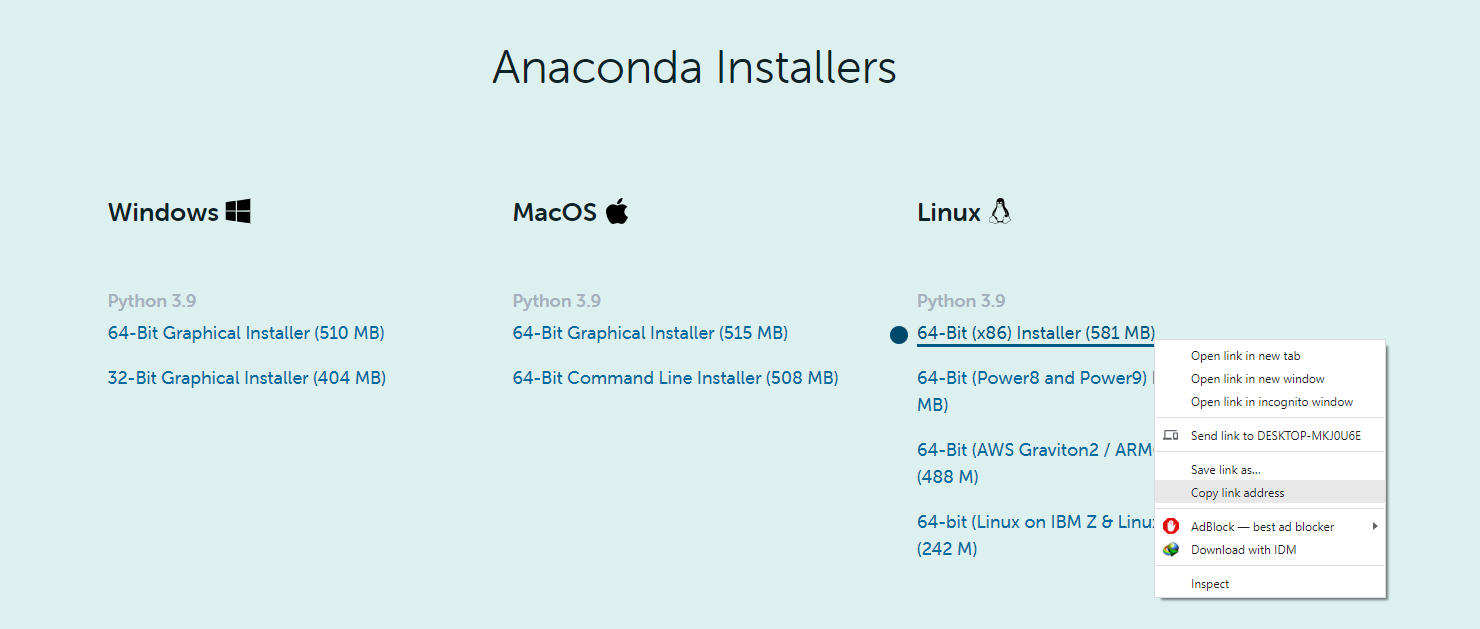
\includegraphics[scale=0.35]{figures/instalasi-anaconda-linux/step1}}
        \caption{Instalasi Anaconda Linux: Step 1}
\end{figure}
\item buka terminal lalu ketikkan \textbf{cd temp/}, tekan enter
\begin{figure}[H]
        \centerline{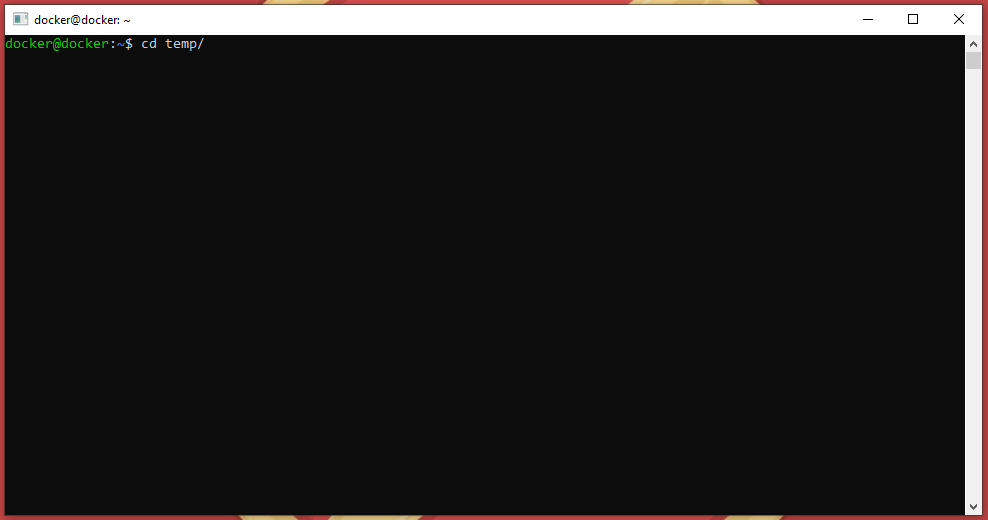
\includegraphics[scale=0.5]{figures/instalasi-anaconda-linux/step2}}
        \caption{Instalasi Anaconda Linux: Step 2}
\end{figure}
\item setelah itu ketikkan \textbf{wget \textit{link yang sudah dicopy}}
\begin{figure}[H]
        \centerline{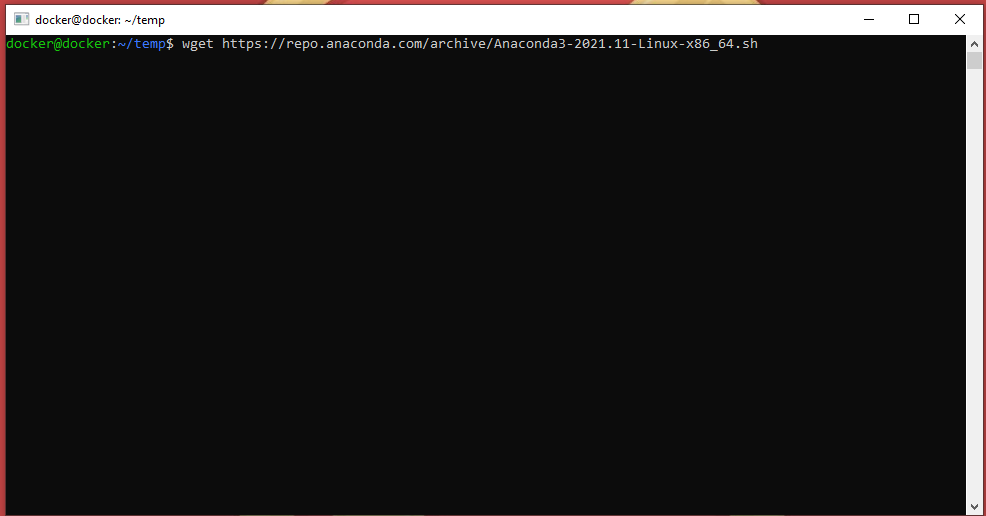
\includegraphics[scale=0.5]{figures/instalasi-anaconda-linux/step3}}
        \caption{Instalasi Anaconda Linux: Step 3}
\end{figure}
\item tekan enter, dan tunggu hingga download selesai
\begin{figure}[H]
        \centerline{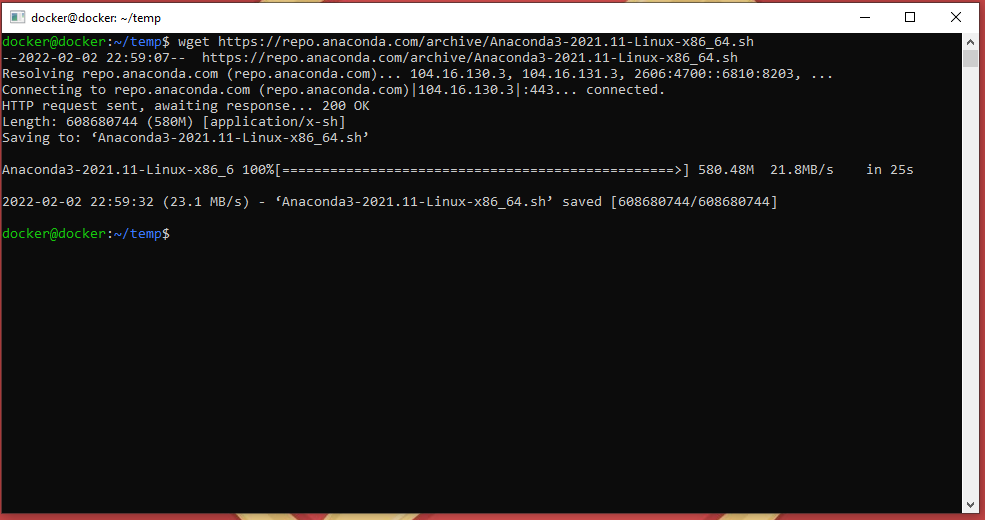
\includegraphics[scale=0.5]{figures/instalasi-anaconda-linux/step4}}
        \caption{Instalasi Anaconda Linux: Step 4}
\end{figure}
\item jika sudah ketikkan \textbf{bash \textit{nama file anaconda, sedikit tips, untuk lebih cepat ketikkan Anac lalu tekan Tab maka secara otomatis akan mengisi nama filenya}}
\begin{figure}[H]
        \centerline{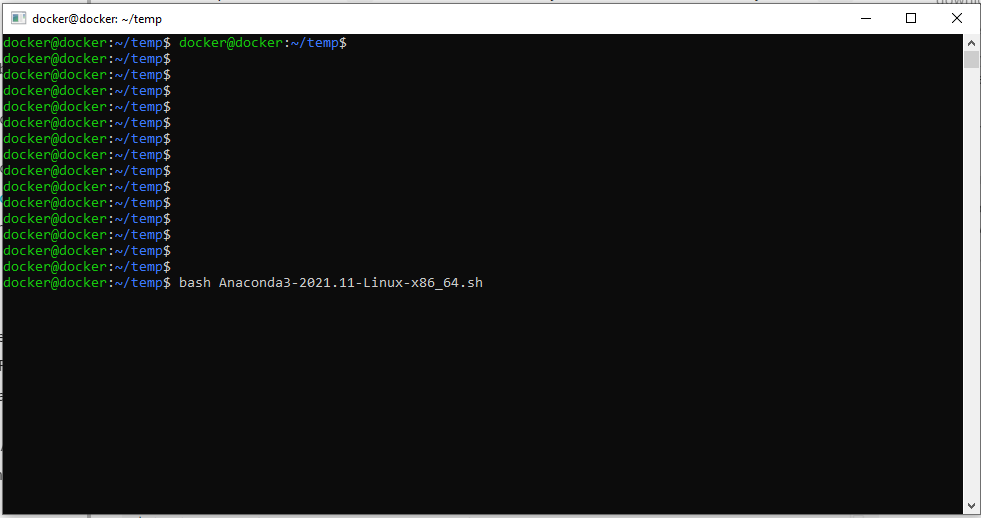
\includegraphics[scale=0.5]{figures/instalasi-anaconda-linux/step5}}
        \caption{Instalasi Anaconda Linux: Step 5}
\end{figure}
\item lalu tekan Enter
\begin{figure}[H]
        \centerline{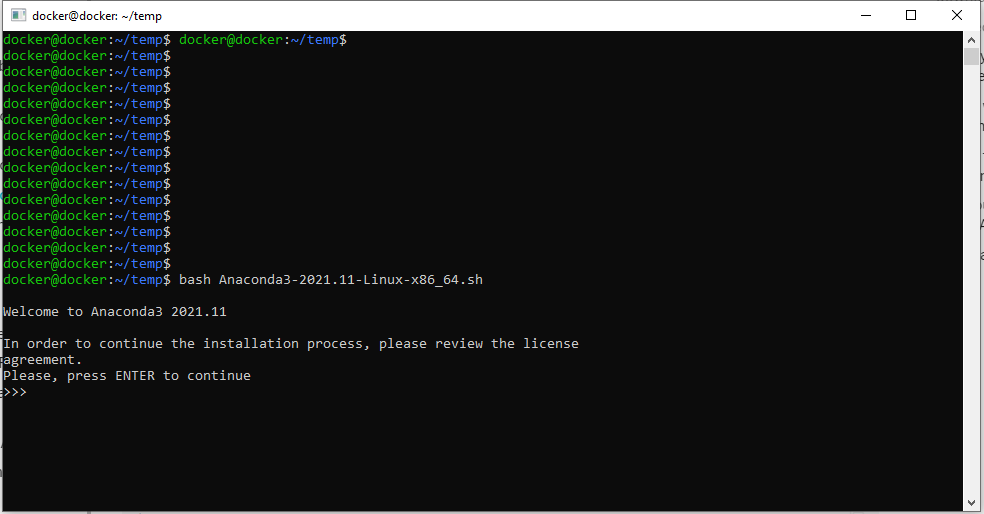
\includegraphics[scale=0.5]{figures/instalasi-anaconda-linux/step6}}
        \caption{Instalasi Anaconda Linux: Step 6}
\end{figure}
\item jika muncul gambar dibawah ini
\begin{figure}[H]
        \centerline{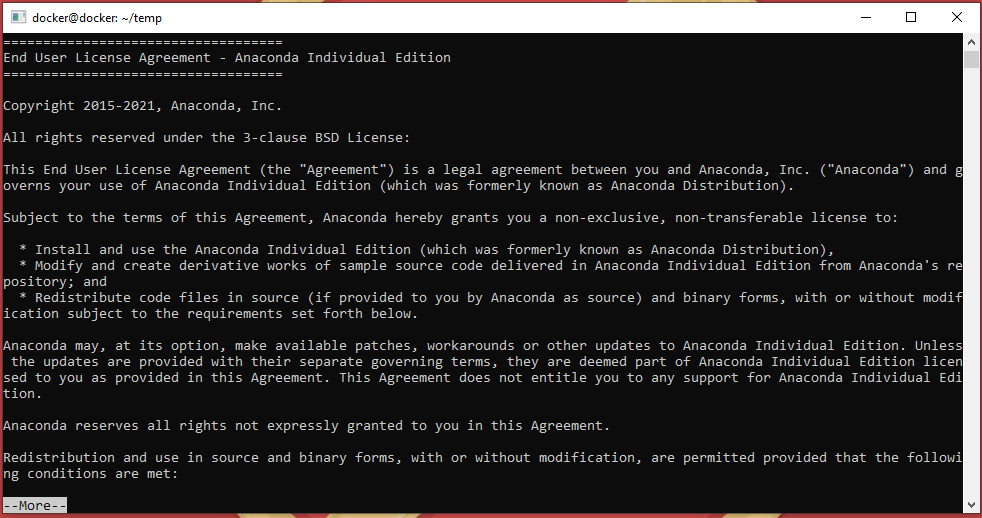
\includegraphics[scale=0.5]{figures/instalasi-anaconda-linux/step7}}
        \caption{Instalasi Anaconda Linux: Step 7}
\end{figure}
\item tekan dan tahan Enter sampai muncul gambar dibawah ini, lalu ketik yes, tekan enter
\begin{figure}[H]
        \centerline{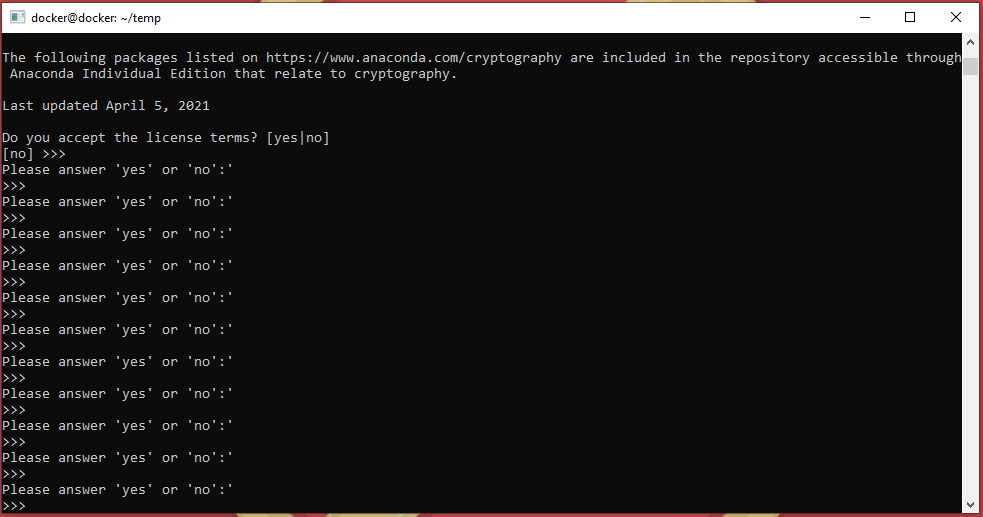
\includegraphics[scale=0.5]{figures/instalasi-anaconda-linux/step8}}
        \caption{Instalasi Anaconda Linux: Step 8}
\end{figure}
\item jika sudah seperti gambar dibawah, tekan enter
\begin{figure}[H]
        \centerline{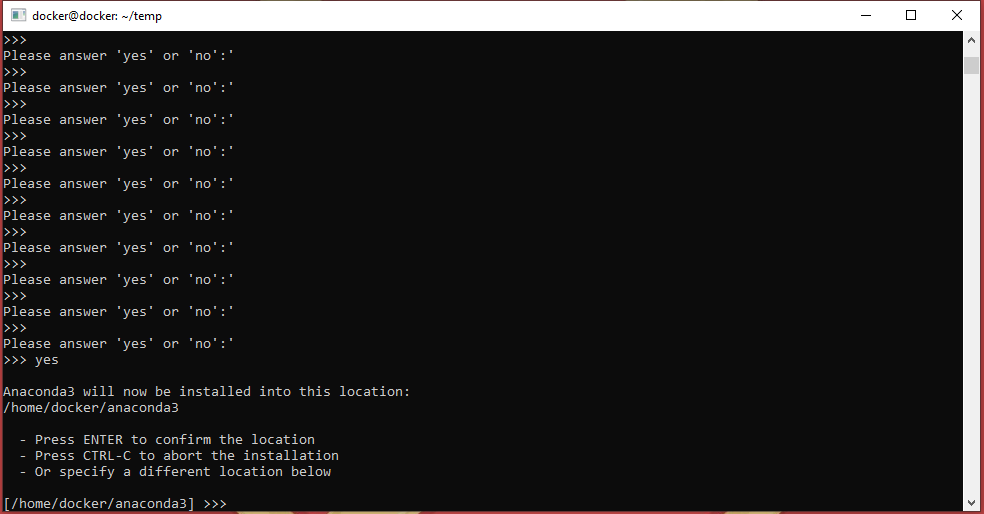
\includegraphics[scale=0.5]{figures/instalasi-anaconda-linux/step9}}
        \caption{Instalasi Anaconda Linux: Step 9}
\end{figure}
\item tunggu hingga proses selesai
\begin{figure}[H]
        \centerline{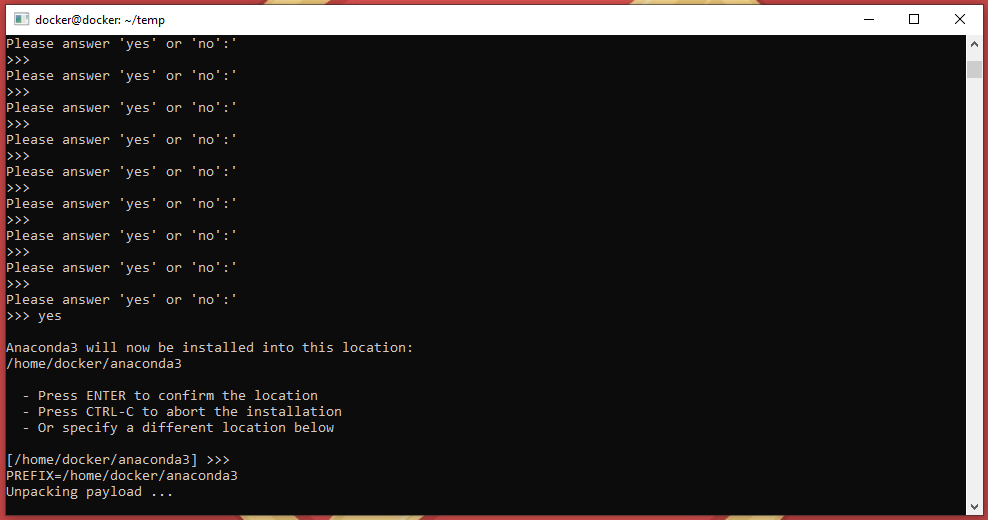
\includegraphics[scale=0.5]{figures/instalasi-anaconda-linux/step10}}
        \caption{Instalasi Anaconda Linux: Step 10}
\end{figure}
\item jika sudah selesai instalasi, ketikkan perintah berikut \textbf{export PYTHONPATH=\$PYTHONPATH:\textit{file path anaconda}} seperti dibawah ini, lalu tekan enter
\begin{figure}[H]
        \centerline{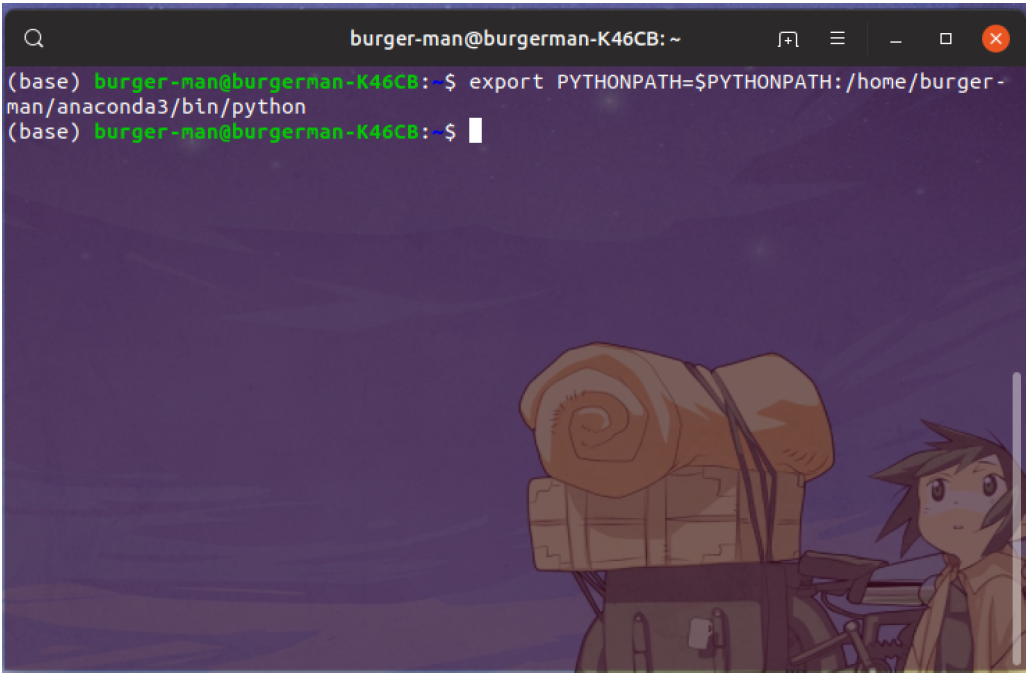
\includegraphics[scale=0.5]{figures/instalasi-anaconda-linux/step11}}
        \caption{Instalasi Anaconda Linux: Step 11}
\end{figure}
\end{enumerate}



\subsection{Windows}
Untuk instalasi python terdapat 2 cara yaitu menggunakan Python langsung atau menggunakan Anaconda

\subsubsection{Python}
\begin{enumerate}
\item Buka browser, kunjungi \url{http://www.python.org/downloads/windows/}
\item Buka (klik 2x) file installer python yang baru saja di download, lalu akan muncul seperti gambar dibawah ini.
\begin{figure}[H]
        \centerline{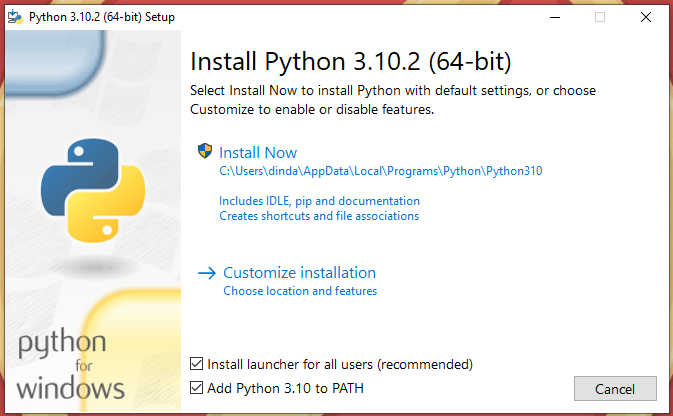
\includegraphics[scale=0.75]{figures/instalasi-python-windows/step1}}
        \caption{Instalasi Python Windows: Step 1}
\end{figure}
\item Pastikan sudah seperti gambar diatas, lalu klik tombol \textbf{Install Now}
\item Lalu akan muncul proses instalasi, tunggu sampai selesai.
\begin{figure}[H]
        \centerline{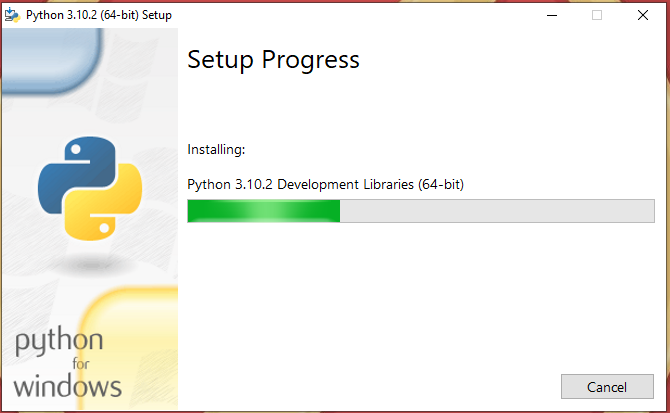
\includegraphics[scale=0.75]{figures/instalasi-python-windows/step2}}
        \caption{Instalasi Python Windows: Step 2}
\end{figure}
\item Jika sudah selesai akan muncul seperti gambar dibawah ini.
\begin{figure}[H]
        \centerline{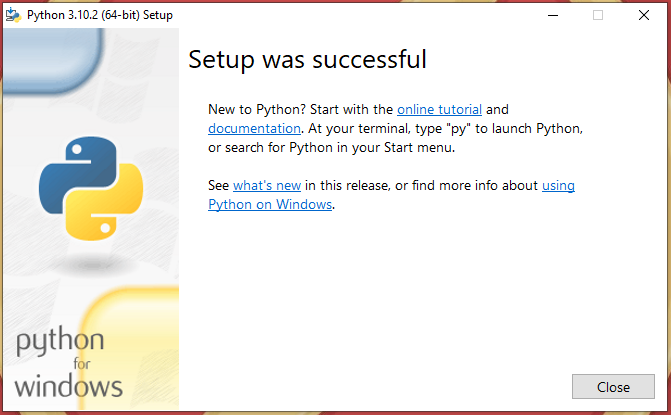
\includegraphics[scale=0.75]{figures/instalasi-python-windows/step3}}
        \caption{Instalasi Python Windows: Step 3}
\end{figure}
\end{enumerate}

\subsubsection{Anaconda}
\begin{enumerate}
\item Buka browser, kunjungi \url{https://www.anaconda.com/products/individual}, lalu download file Installer Anaconda sesuai Bit komputer/laptop anda.
\item Jika sudah download, klik (2x) filenya dan akan muncul seperti gambar dibawah ini.
\begin{figure}[H]
        \centerline{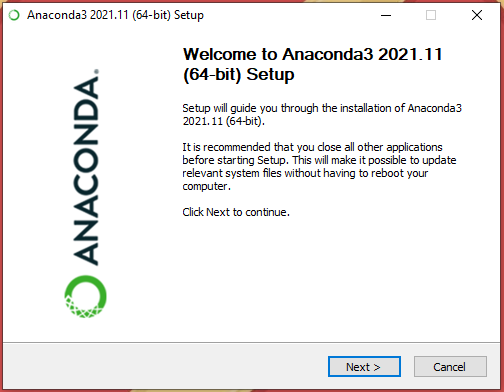
\includegraphics[scale=0.75]{figures/instalasi-anaconda-windows/step1}}
        \label{instalanacondawindowsstep1}
\end{figure}
\item Klik next setelah itu akan muncul seperti gambar dibawah ini.
\begin{figure}[H]
        \centerline{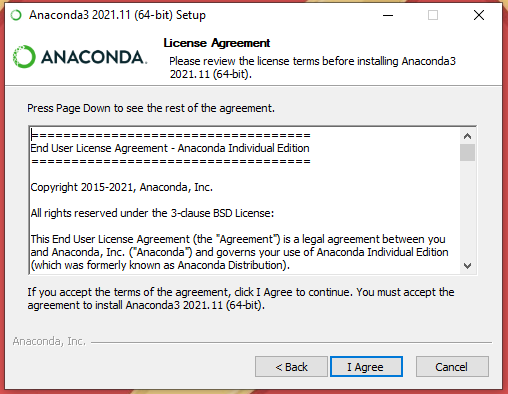
\includegraphics[scale=0.75]{figures/instalasi-anaconda-windows/step2}}
        \label{instalanacondawindowsstep2}
\end{figure}
\item klik I Agree, lalu akan muncul gambar dibawah ini.
\begin{figure}[H]
        \centerline{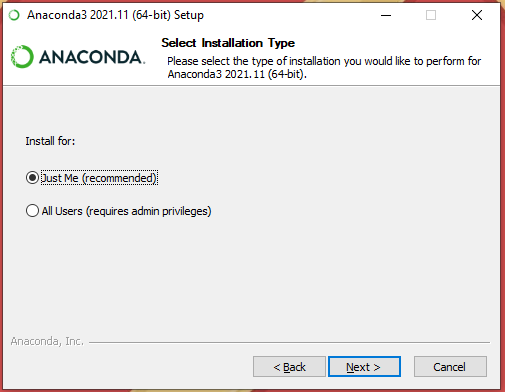
\includegraphics[scale=0.75]{figures/instalasi-anaconda-windows/step3}}
        \label{instalanacondawindowsstep3}
\end{figure}
\item lalu ada pilihan Just Me atau All Users, disini boleh bebas pilih yang mana saja, disini saya memilih Just Me karena direkomendasikan oleh Anacondanya, jika sudah memilih langsung klik next
\begin{figure}[H]
        \centerline{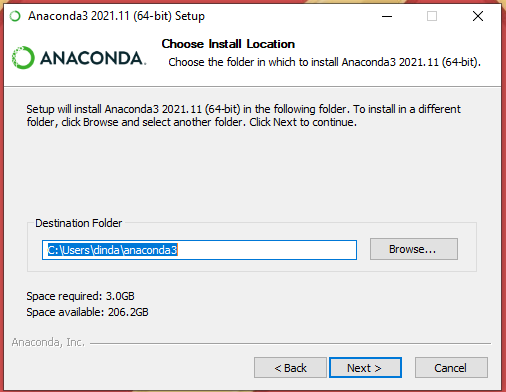
\includegraphics[scale=0.75]{figures/instalasi-anaconda-windows/step4}}
        \label{instalanacondawindowsstep4}
\end{figure}
\item setelah itu muncul destination folder adalah lokasi dimana ekstraksi file Anaconda akan diletakkan dimana, disini saya membiarkan seperti yang sudah diset default oleh Anaconda, klik next
\begin{figure}[H]
        \centerline{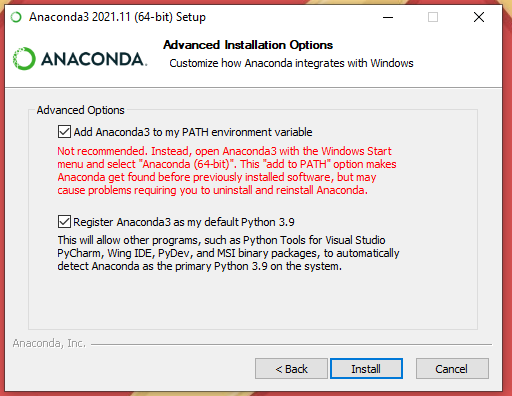
\includegraphics[scale=0.75]{figures/instalasi-anaconda-windows/step5}}
        \label{instalanacondawindowsstep5}
\end{figure}
\item setelah itu muncuk Menu Advanced Options, disini saya mencentang option Add Anaconda3 to my PATH environtment variabel, setelah itu klik install
\begin{figure}[H]
        \centerline{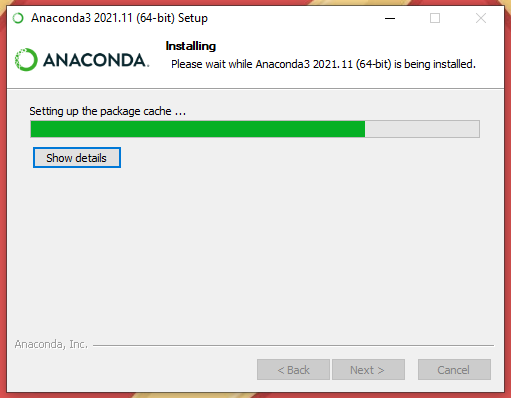
\includegraphics[scale=0.75]{figures/instalasi-anaconda-windows/step6}}
        \label{instalanacondawindowsstep6}
\end{figure}
\item tunggu proses instalasi hingga selesai
\begin{figure}[H]
        \centerline{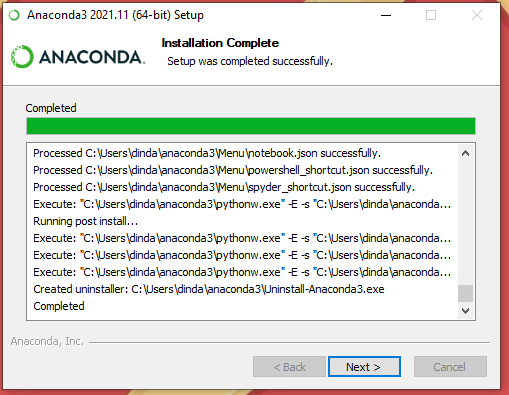
\includegraphics[scale=0.75]{figures/instalasi-anaconda-windows/step7}}
        \caption{Instalasi Anaconda Windows: Step 7}
\end{figure}
\item jika sudah muncul tulisan \textbf{Completed}, klik Next
\begin{figure}[H]
        \centerline{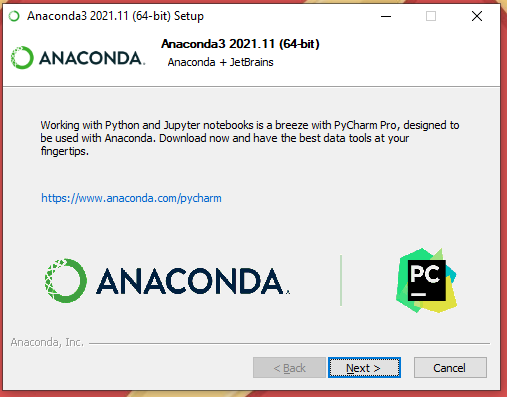
\includegraphics[scale=0.75]{figures/instalasi-anaconda-windows/step8}}
        \caption{Instalasi Anaconda Windows: Step 8}
\end{figure}
\item instalasi anaconda di windows 10 sudah selesai, klik next
\begin{figure}[H]
        \centerline{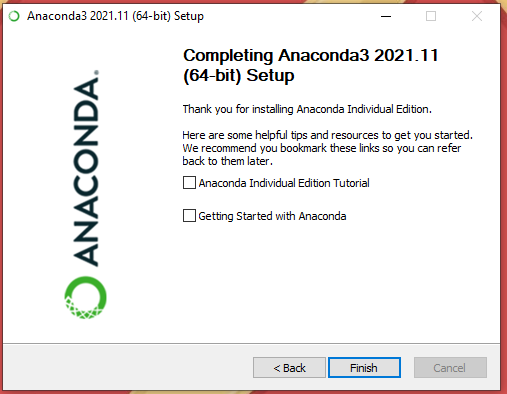
\includegraphics[scale=0.75]{figures/instalasi-anaconda-windows/step9}}
        \caption{Instalasi Anaconda Windows: Step 9}
\end{figure}
\item jika ingin mengunjungi website anaconda dan membaca manual secara lengkap boleh di centang kedua opsinya dan klik Finish, disini saya tidak mencentang kedua opsi.
\end{enumerate}

\section{Menjalankan Python}
Untuk menjalankan Python ada banyak cara yang bisa dilakukan. Anda bisa menggunakan \textit{shell}, terminal atau menggunakan IDE (Integrated Development Environment). Di bawah ini adalah langkah-langkah menjalankan Python dengan cara yang paling mudah.

\subsection{Linux}
\begin{enumerate}
\item Buka terminal CTRL + ALT + T
\begin{figure}[H]
        \centerline{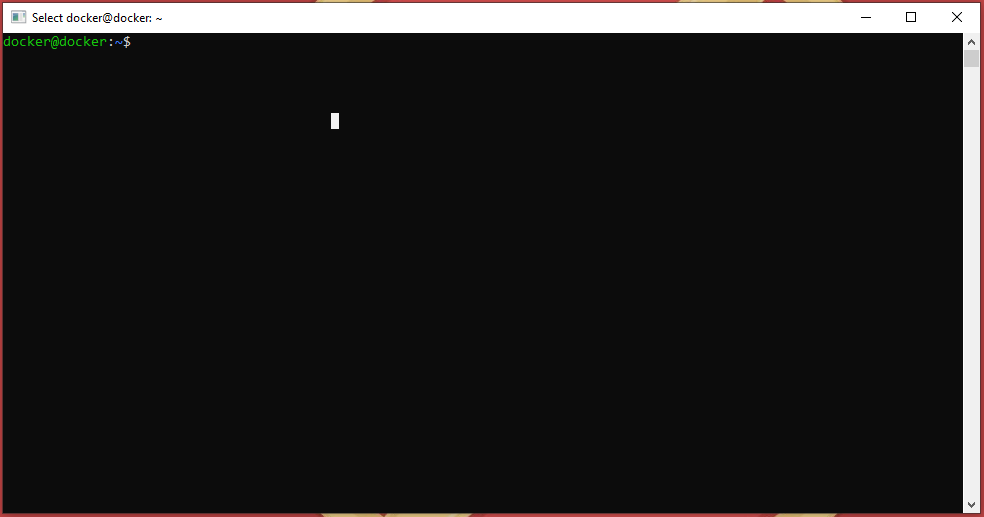
\includegraphics[scale=0.5]{figures/menjalankan-python-linux/step1}}
        \caption{Menjalankan Python Linux: Step 1}
\end{figure}
\item ketik \textbf{python3} lalu tekan enter
\begin{figure}[H]
        \centerline{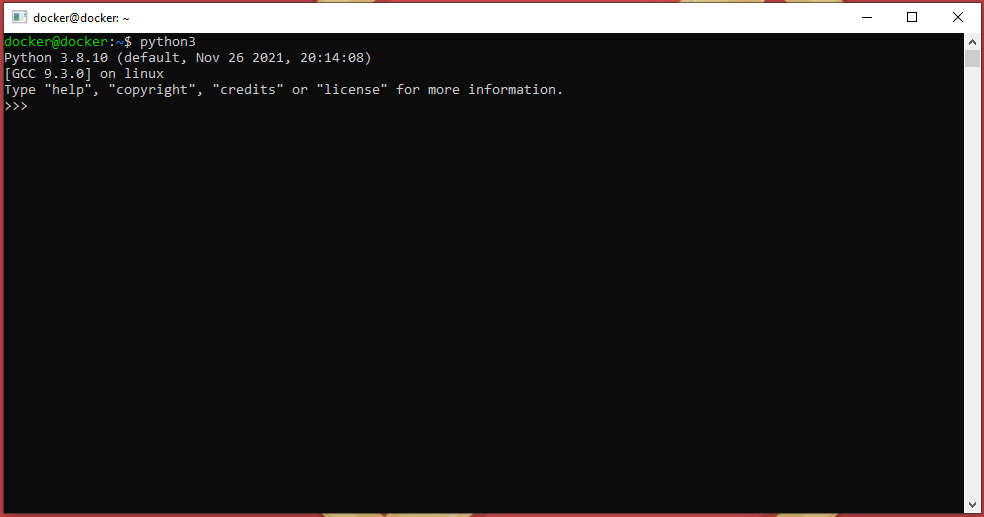
\includegraphics[scale=0.5]{figures/menjalankan-python-linux/step2}}
        \caption{Menjalankan Python Linux: Step 2}
\end{figure}
\item ketik \textbf{print("hello world")} tekan enter
\begin{figure}[H]
        \centerline{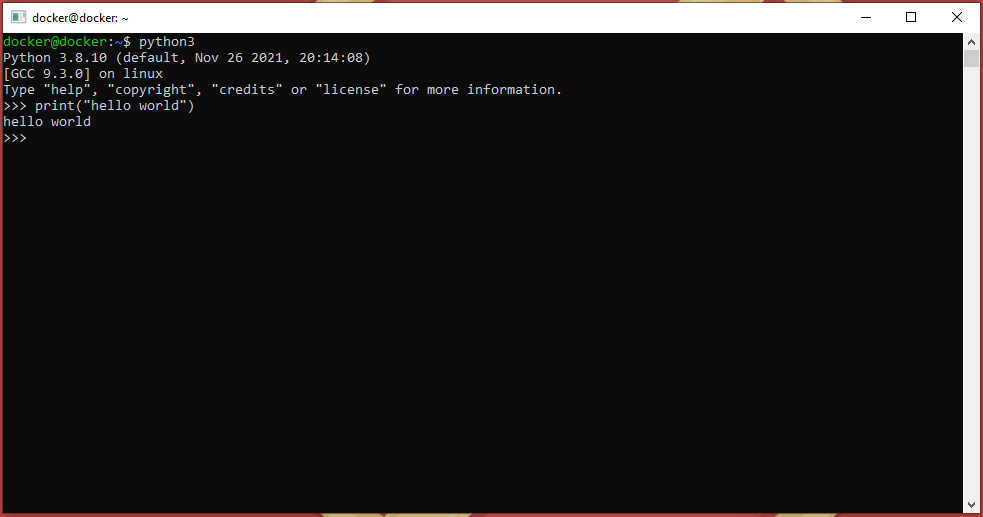
\includegraphics[scale=0.5]{figures/menjalankan-python-linux/step3}}
        \caption{Menjalankan Python Linux: Step 3}
\end{figure}
\item selamat anda sudah berhasil menjalankan program python3
\item jika ingin keluar dari shell python3 bisa dengan mengetik \textbf{exit()} lalu enter
\begin{figure}[H]
        \centerline{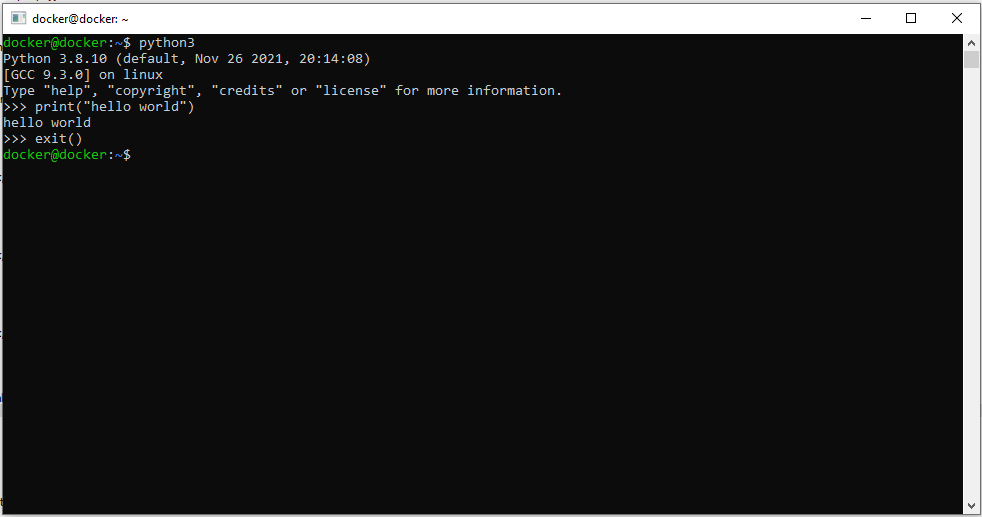
\includegraphics[scale=0.5]{figures/menjalankan-python-linux/step4}}
        \caption{Menjalankan Python Linux: Step 4}
\end{figure}
\end{enumerate}

\textit{atau}

\begin{enumerate}
\item Gunakan teks editor, misalnya \textbf{nano cetak.py}
\begin{figure}[H]
        \centerline{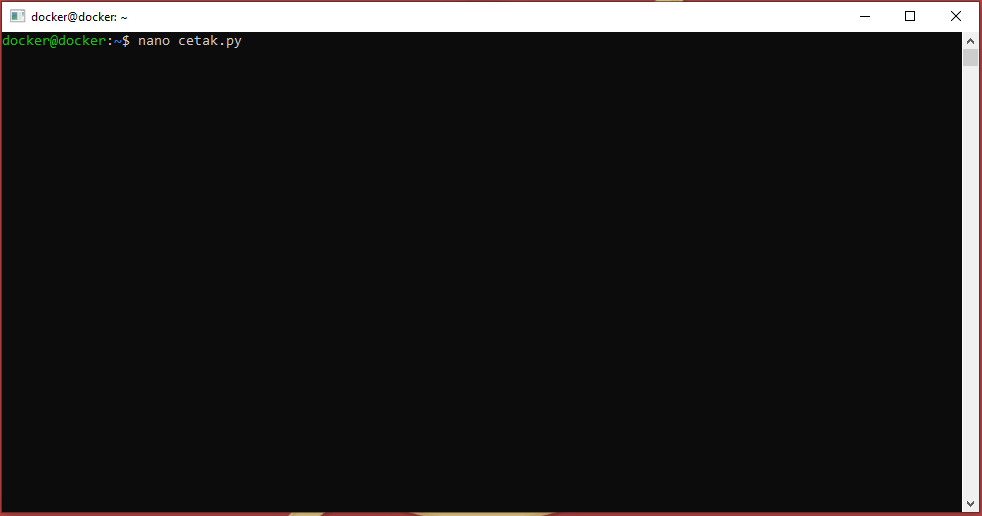
\includegraphics[scale=0.5]{figures/menjalankan-python-linux-with-nano/step1}}
        \caption{Menjalankan Python Linux dengan Teks Editor: Step 1}
\end{figure}
\item ketik \textbf{print("Selamat datang di Python")}
\begin{figure}[H]
        \centerline{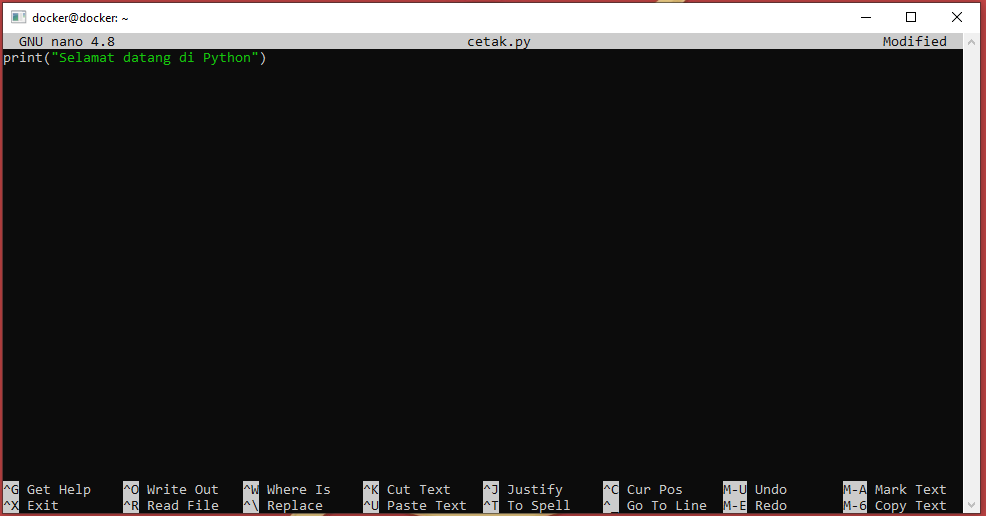
\includegraphics[scale=0.5]{figures/menjalankan-python-linux-with-nano/step2}}
        \caption{Menjalankan Python Linux dengan Teks Editor: Step 2}
\end{figure}
\item lalu tekan tombol CTRL + X
\begin{figure}[H]
        \centerline{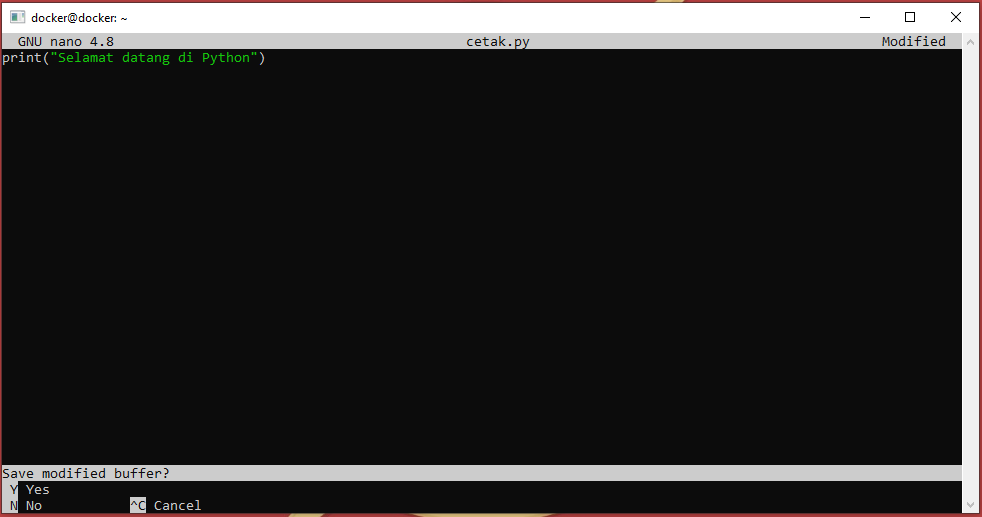
\includegraphics[scale=0.5]{figures/menjalankan-python-linux-with-nano/step3}}
        \caption{Menjalankan Python Linux dengan Teks Editor: Step 3}
\end{figure}
\item setelah itu tekan tombol \textbf{y}
\begin{figure}[H]
        \centerline{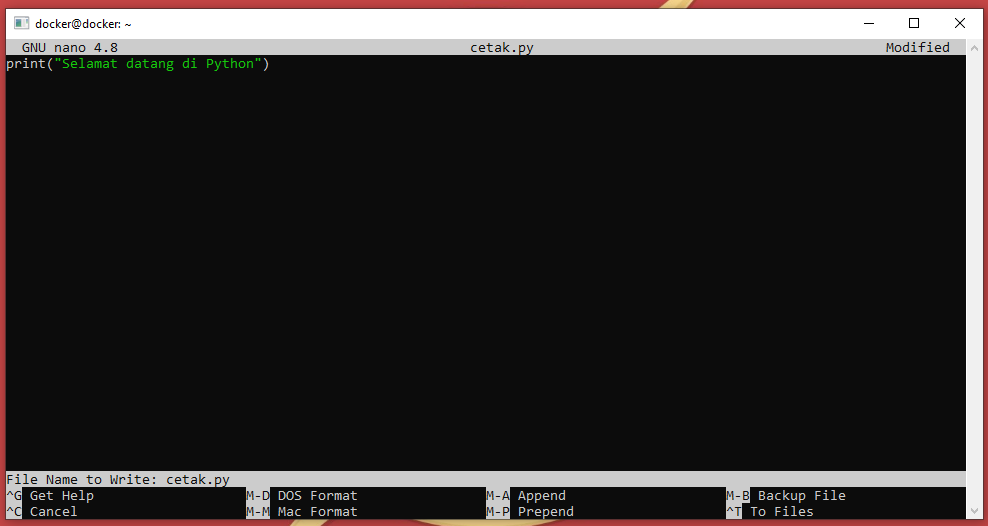
\includegraphics[scale=0.5]{figures/menjalankan-python-linux-with-nano/step4}}
        \caption{Menjalankan Python Linux dengan Teks Editor: Step 4}
\end{figure}
\item lalu tekan Enter
\begin{figure}[H]
        \centerline{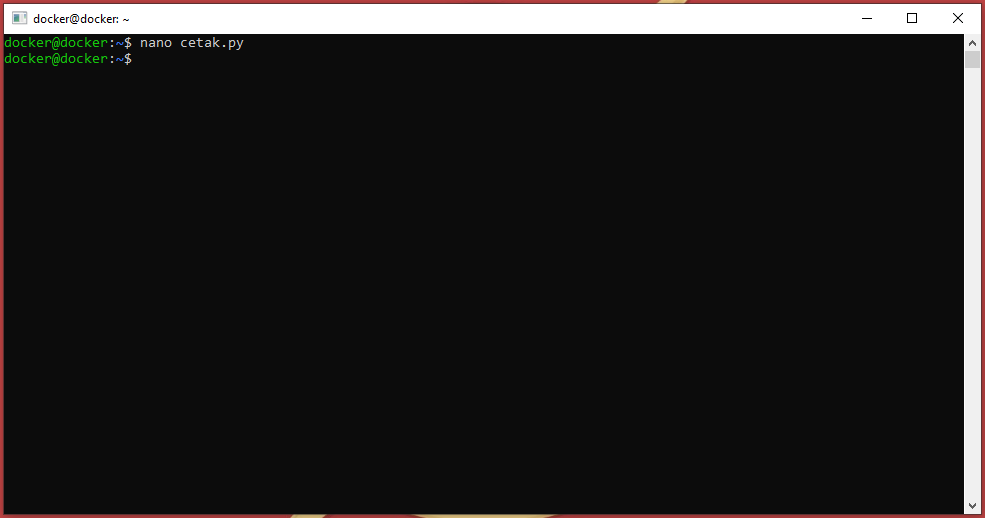
\includegraphics[scale=0.5]{figures/menjalankan-python-linux-with-nano/step5}}
        \caption{Menjalankan Python Linux dengan Teks Editor: Step 5}
\end{figure}
\item lalu ketikkan \textbf{python3 cetak.py}
\begin{figure}[H]
        \centerline{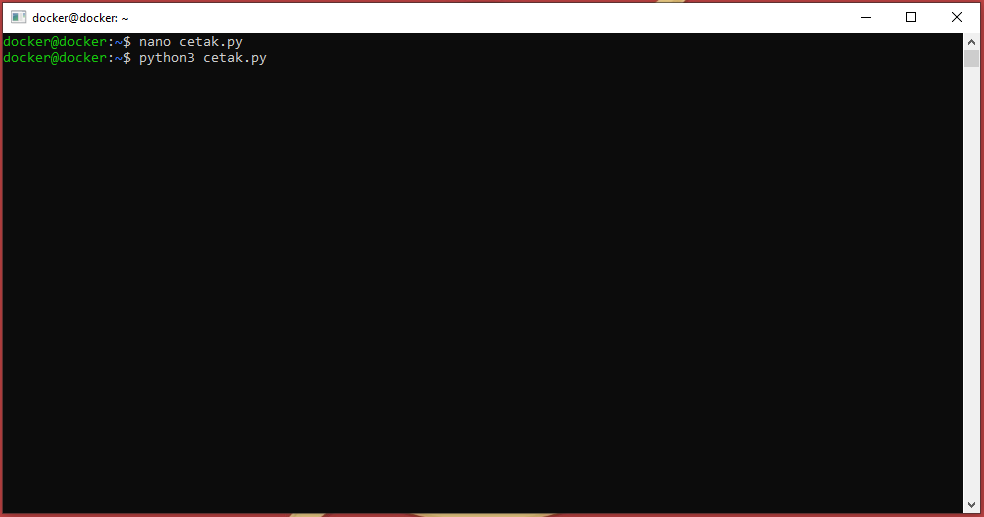
\includegraphics[scale=0.5]{figures/menjalankan-python-linux-with-nano/step6}}
        \caption{Menjalankan Python Linux dengan Teks Editor: Step 6}
\end{figure}
\item lalu tekan Enter
\begin{figure}[H]
        \centerline{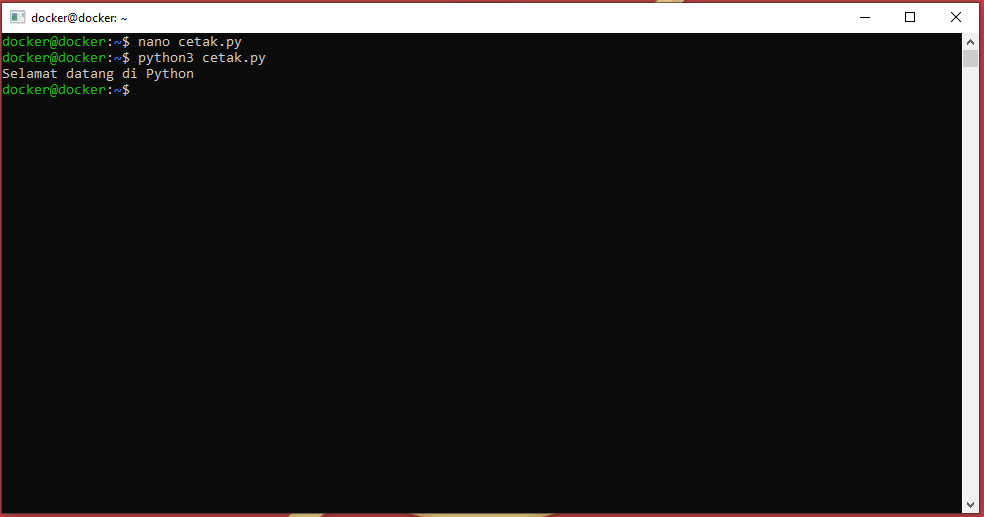
\includegraphics[scale=0.5]{figures/menjalankan-python-linux-with-nano/step7}}
        \caption{Menjalankan Python Linux dengan Teks Editor: Step 7}
\end{figure}
\end{enumerate}

\subsection{Windows}
\subsubsection{Menggunakan Shell}
\begin{enumerate}
\item Buka IDLE (python shell di windows), Anda bisa mencarinya di tombol START.
\item Tuliskan script Python Anda, contoh: print("Selamat datang di Python"). jika sudah tekan tombol ENTER, dan script Python akan dijalankan/eksekusi.
\begin{figure}[H]
        \centerline{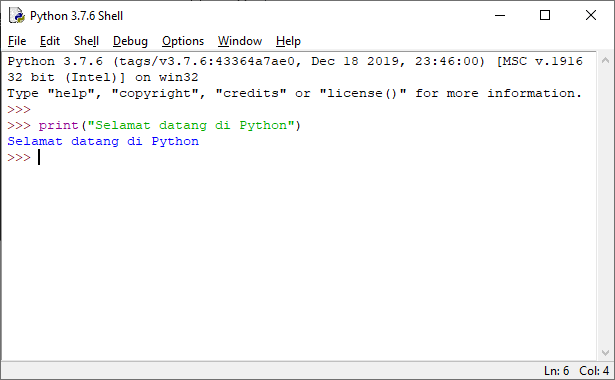
\includegraphics[scale=0.75]{figures/menjalankan-python-windows/step1}}
        \caption{Menjalankan Python Windows}
        \label{windowsshellpython}
\end{figure}
\item Untuk keluar dari Python shell ketik exit()
\end{enumerate}

\subsubsection{Menggunakan Script Editor}
\begin{enumerate}
\item Untuk menjalankan script yang disimpan dalam file, buka IDLE (python shell di windows), Anda bisa mencarinya di tombol START.
\item Klik menu File - New File
\item Tulis script Python pada window yang muncul, contoh:
\begin{lstlisting}[language=Python]
print("Belajar Python")
\end{lstlisting}
\item Simpan script lewat menu File - Save
\item Jalankan program dengan klik menu Run - Run Module
\end{enumerate}

\section{Hello World}
Syntax bahasa Python hampir sama dengan bahasa pemrograman pada umumnya seperti Java atau PHP.

\subsection{Syntax Dasar}
Dibawah ini adalah contoh fungsi Python yang digunakan untuk mencetak. Di Python untuk mencetak cukup gunakan fungsi print() , dimana sesuatu yang akan dicetak harus diletakkan diantara kurung buka dan kurung tutup, bahkan di Python versi 2.x Anda tidak harus menggunakan tanda kurung kurawal, cukup pisahkan dengan spasi. Jika ingin mencetak tipe data String langsung, Anda harus memasukanya ke dalam tanda kutip terlebih dahulu.
\begin{lstlisting}[language=Python]
print("Hello World")
\end{lstlisting}
Saat anda menjalankan script diatas, Anda akan melihat output berupa text Hello World.

\subsection{Python Case Sensitivity}
Python bersifat case sensitif, ini artinya huruf besar dan huruf kecil memiliki perbedaan. Sebagai contoh jika Anda menggunakan fungsi print dengan huruf kecil print() akan berhasil. Lain hal jika anda menggunakan huruf kapital Print() atau PRINT() , akan muncul pesan error. Aturan ini berlaku untuk nama variabel ataupun fungsi-fungsi lainnya.

\section{Komentar Python}
Komentar (comment) adalah kode di dalam script Python yang tidak dieksekusi atau tidak dijalankan mesin. Komentar hanya digunakan untuk menandai atau memberikan keterangan tertulis pada script. Komentar biasa digunakan untuk membiarkan orang lain memahami apa yang dilakukan script. atau untuk mengingatkan kepada programmer sendiri jika suatu saat kembali mengedit script tersebut. Untuk menggunakan komentar anda cukup menulis tanda pagar \#, diikuti dengan komentar Anda. Dibawah ini adalah contoh penggunaan komentar pada Python.
\lstinputlisting[caption=Python Comment, language=Python]{src/komentar.py}
Saat anda menjalankan script diatas, Anda akan melihat output berupa Hello World, Budi dan 123, karena tulisan/komentar yang ditulis tidak dieksekusi.

\section{Tipe Data Python}
Tipe data adalah suatu media atau memori pada komputer yang digunakan untuk menampung informasi. Python sendiri mempunyai tipe data yang cukup unik bila kita bandingkan dengan bahasa pemrograman yang lain. Berikut adalah tipe data dari bahasa pemrograman Python :

\begin{center}
\begin{tabular}{ | m{2cm} | m{2cm} | m{7cm} | }
\hline
Tipe Data & Contoh & Penjelasan \\
\hline
Boolean & \textbf{True} atau \textbf{False} & Menyatakan benar \textbf{True} yang bernilai \textbf{1}, atau salah \textbf{False} yang bernilai \textbf{0} \\
\hline
String & "Ayo belajar Python" & Menyatakan karakter/kalimat bisa berupa huruf angka, dll (diapit tanda " atau ') \\
\hline
Integer & 10 atau 100 & Menyatakan bilangan bulat \\
\hline
Float & 3.14 atau 1.22 & Menyatakan bilangan yang mempunyai koma \\
\hline
Hexadecimal & 9a atau 1d3 & Menyatakan bilangan dalam format heksa (bilangan berbasis 16) \\
\hline
Complex & 1 + 5j & Menyatakan pasangan angka real dan imajiner \\
\hline
List & ['tri', 'angga', 'dio', 'simamora'] atau [1, 2, 3, 4] & Data untaian yang menyimpan berbagai tipe data dan isinya bisa diubah atau modifikasi \\
\hline
Tuple & ('tri', 'angga', 'dio', 'simamora') atau (1, 2, 3, 4) & Data untaian yang menyimpan berbagai tipe data dan isinya tidak bisa diubah atau modifikasi \\
\hline
Dictionary & \{'nama': 'tri angga dio simamora'\} & Data untaian yang menyimpan berbagai tipe data berupa pasangan key dan value \\
\hline
\end{tabular}
\end{center}

Untuk mencoba berbagai macam tipe data, silahkan coba script Python dibawah ini.
\lstinputlisting[caption=Python Tipe Data, language=Python]{src/tipe_data.py}

\section{Variabel Python}
Variabel adalah lokasi memori yang dicadangkan untuk menyimpan nilai-nilai. Ini berarti bahwa ketika Anda membuat sebuah variabel Anda memesan beberapa ruang di memori. Variabel menyimpan data yang dilakukan selama program dieksekusi, yang nantinya isi dari variabel tersebut dapat diubah oleh operasi - operasi tertentu pada program yang menggunakan variabel.

Variabel dapat menyimpan berbagai macam tipe data. Di dalam pemrograman Python, variabel mempunyai sifat yang dinamis, artinya variabel Python tidak perlu didekralasikan tipe data tertentu dan variabel Python dapat diubah saat program dijalankan.

Penulisan variabel Python sendiri juga memiliki aturan tertentu, yaitu :

\begin{enumerate}
\item Karakter pertama harus berupa huruf atau garis bawah/underscore \textbf{\_}
\item Karakter selanjutnya dapat berupa huruf, garis bawah/underscore \textbf{\_} atau angka
\item Karakter pada nama variabel bersifat sensitif (case-sensitif). Artinya huruf kecil dan huruf besar dibedakan. Sebagai contoh, \textbf{namaDepan} dan \textbf{namadepan} adalah variabel yang berbeda.
\end{enumerate}

Untuk mulai membuat variabel di Python caranya sangat mudah, Anda cukup menuliskan variabel lalu mengisinya dengan suatu nilai dengan cara menambahkan tanda sama dengan \textbf{=} diikuti dengan nilai yang ingin dimasukan.

Dibawah ini adalah contoh penggunaan variabel dalam bahasa pemrograman Python
\lstinputlisting[caption=Python Variabel, language=Python]{src/variabel.py}

\section{Operator Python}
Operator adalah konstruksi yang dapat memanipulasi nilai dari operan. Sebagai contoh operasi 3 + 2 = 5. Disini 3 dan 2 adalah operan dan + adalah operator. Bahasa pemrograman Python mendukung berbagai macam operator, diantaranya :


\subsection{Operator Aritmatika}
\begin{center}
\begin{tabular}{ | m{2cm} | m{2cm} | m{7cm} | }
\hline
Operator & Contoh & Penjelasan \\
\hline
Penjumlahan & 1 + 3 = 4 & Menjumlahkan nilai dari masing-masing operan atau bilangan \\
\hline
Pengurangan & 4 - 1 = 3 & Mengurangi nilai operan di sebelah kiri menggunakan operan di sebelah kanan \\
\hline
Perkalian & 2 * 4 = 8 & Mengalikan operan/bilangan \\
\hline
Pembagian & 10 / 5 = 2 & Untuk membagi operan di sebelah kiri menggunakan operan di sebelah kanan \\
\hline
Sisa Bagi (Modulo) & 11 \% 2 = 1 & Mendapatkan sisa pembagian dari operan di sebelah kiri operator ketika dibagi oleh operan di sebelah kanan \\
\hline
Pangkat & 8 ** 2 = 64 & Memangkatkan operan disebelah kiri operator dengan operan di sebelah kanan operator \\
\hline
Pembagian Bulat & 10 // 3 = 3 & Sama seperti pembagian. Hanya saja angka dibelakang koma dihilangkan \\
\hline
\end{tabular}
\end{center}
Dibawah ini adalah contoh penggunaan Operator Aritmatika dalam bahasa pemrograman Python
\lstinputlisting[caption=Python Operator Aritmatika, language=Python]{src/aritmatika.py}

\subsection{Operator Perbandingan}
\begin{center}
\begin{tabular}{ | m{2cm} | m{2cm} | m{7cm} | }
\hline
Operator & Contoh & Penjelasan \\
\hline
Sama dengan & 1 == 1 & bernilai True Jika masing-masing operan memiliki nilai yang sama, maka kondisi bernilai benar atau True. \\
\hline
Tidak sama dengan & 2 != 2 & bernilai False Akan menghasilkan nilai kebalikan dari kondisi sebenarnya. \\
\hline
Tidak sama dengan & 2 \texttt{<>} 2 & bernilai False Akan menghasilkan nilai kebalikan dari kondisi sebenarnya. \\
\hline
Lebih besar dari & 5 \texttt{>} 3 & bernilai True Jika nilai operan kiri lebih besar dari nilai operan kanan, maka kondisi menjadi benar. \\
\hline
Lebih kecil dari & 5 \texttt{<} 3 & bernilai True Jika nilai operan kiri lebih kecil dari nilai operan kanan, maka kondisi menjadi benar. \\
\hline
Lebih besar atau sama dengan & 5 \texttt{>}= 3 & bernilai True Jika nilai operan kiri lebih besar dari nilai operan kanan, atau sama, maka kondisi menjadi benar. \\
\hline
Lebih kecil atau sama dengan & 5 \texttt{<}= 3 & bernilai True Jika nilai operan kiri lebih kecil dari nilai operan kanan, atau sama, maka kondisi menjadi benar. \\
\hline
\end{tabular}
\end{center}

\subsection{Operator Penugasan}
Operator penugasan digunakan untuk memberikan atau memodifikasi nilai ke dalam sebuah variabel.
\begin{center}
\begin{tabular}{ | m{2cm} | m{2cm} | m{7cm} | }
\hline
Operator & Contoh & Penjelasan \\
\hline
Sama dengan & a = 1 & Memberikan nilai di kanan ke dalam variabel yang berada di sebelah kiri. \\
\hline
Tambah sama dengann & a += 2 & Memberikan nilai variabel dengan nilai variabel itu sendiri ditambah dengan nilai di sebelah kanan. \\
\hline
Kurang sama dengan & a -= 2 & Memberikan nilai variabel dengan nilai variabel itu sendiri dikurangi dengan nilai di sebelah kanan. \\
\hline
Kali sama dengan & a *= 2 & Memberikan nilai variabel dengan nilai variabel itu sendiri dikali dengan nilai di sebelah kanan. \\
\hline
Bagi sama dengan & a /= 4 & Memberikan nilai variabel dengan nilai variabel itu sendiri dibagi dengan nilai di sebelah kanan. \\
\hline
Sisa bagi sama dengan & a \%= 3 & Memberikan nilai variabel dengan nilai variabel itu sendiri dibagi dengan nilai di sebelah kanan. Yang diambil nantinya adalah sisa baginya.\\
\hline
Pangkat sama dengan & a **= 3 & Memberikan nilai variabel dengan nilai variabel itu sendiri dipangkatkan dengan nilai di sebelah kanan. \\
\hline
Pembagian bulat sama dengan & a //= 3 & Membagi bulat operan sebelah kiri operator dengan operan sebelah kanan operator kemudian hasilnya diisikan ke operan sebelah kiri. \\
\hline
\end{tabular}
\end{center}

\subsection{Prioritas Eksekusi Operator di Python}
Dari semua operator diatas, masing-masing mempunyai urutan prioritas yang nantinya prioritas pertama akan dilakukan paling pertama, begitu seterusnya sampai dengan prioritas terakhir.
\begin{center}
\begin{tabular}{ | m{4cm} | m{4cm} | }
\hline
Operator & Keterangan \\
\hline
** & Aritmatika \\
\hline
~, +, - & Bitwise \\
\hline
*, /, \%, // & Aritmatika \\
\hline
+, - & Aritmatika \\
\hline
\texttt{>>}, \texttt{<<} & Bitwise \\
\hline
\& & Bitwise \\
\hline
\^, | & Bitwise \\
\hline
\texttt{<}=, \texttt{<}, \texttt{>}, \texttt{>}= & Perbandingan \\
\hline
\texttt{<>} , ==, != & Perbandingan \\
\hline
=, \%=, /=, //=, -=, +=, *=, **= & Penugasan \\
\hline
is, is not & Identitas \\
\hline
in, not in & Membership (Keanggotaan) \\
\hline
not, or, and & Logika \\
\hline
\end{tabular}
\end{center}


\section{Kondisi Python}

\subsection{Kondisi If}
Pengambilan keputusan (kondisi if) digunakan untuk mengantisipasi kondisi yang terjadi saat jalanya program dan menentukan tindakan apa yang akan diambil sesuai dengan kondisi. Pada python ada beberapa statement/kondisi diantaranya adalah if, else dan elif Kondisi if digunakan untuk mengeksekusi kode jika kondisi bernilai benar True. Jika kondisi bernilai salah False maka statement/kondisi if tidak akan di-eksekusi. Dibawah ini adalah contoh penggunaan kondisi if pada Python
\lstinputlisting[caption=Python Kondisi If, language=Python]{src/if.py}
Dari contoh diatas, jika program dijalankan maka akan mencetak string "Sembilan Lebih Besar Dari Angka Tujuh" sebanyak 1 kali yaitu pada if pertama. Di if kedua statement bernilai salah, jadi perintah print("Sembilan Lebih Besar Dari Angka Sepuluh") tidak akan dieksekusi.

\subsection{Kondisi If Else}
Pengambilan keputusan (kondisi if else) tidak hanya digunakan untuk menentukan tindakan apa yang akan diambil sesuai dengan kondisi, tetapi juga digunakan untuk menentukan tindakan apa yang akan diambil/dijalankan jika kondisi tidak sesuai. Pada python ada beberapa statement/kondisi diantaranya adalah if, else dan elif Kondisi if digunakan untuk mengeksekusi kode jika kondisi bernilai benar. Kondisi if else adalah kondisi dimana jika pernyataan benar True maka kode dalam if akan dieksekusi, tetapi jika bernilai salah False maka akan mengeksekusi kode di dalam else. Dibawah ini adalah contoh penggunaan kondisi if else pada Python
\lstinputlisting[caption=Python Kondisi If Else, language=Python]{src/ifelse.py}
Pada contoh diatas, jika program dijalankan maka akan mencetak string "Maaf Anda Tidak Lulus" karena pernyataan pada if bernilai False

\subsection{Kondisi Elif}
Pengambilan keputusan (kondisi if elif) merupakan lanjutan/percabangan logika dari “kondisi if”. Dengan elif kita bisa membuat kode program yang akan menyeleksi beberapa kemungkinan yang bisa terjadi. Hampir sama dengan kondisi “else”, bedanya kondisi “elif” bisa banyak dan tidak hanya satu.

Dibawah ini adalah contoh penggunaan kondisi elif pada Python
\lstinputlisting[caption=Python Kondisi Elif, language=Python]{src/elif.py}
Pada contoh diatas, jika program dijalankan maka akan mencetak string "Saya akan libur".

\section{Loop Python}
Secara umum, pernyataan pada bahasa pemrograman akan dieksekusi secara berurutan. Pernyataan pertama dalam sebuah fungsi dijalankan pertama, diikuti oleh yang kedua, dan seterusnya. Tetapi akan ada situasi dimana Anda harus menulis banyak kode, dimana kode tersebut sangat banyak. Jika dilakukan secara manual maka Anda hanya akan membuang-buang tenaga dengan menulis beratus-ratus bahkan beribu-ribu kode. Untuk itu Anda perlu menggunakan pengulangan di dalam bahasa pemrograman Python.

Di dalam bahasa pemrograman Python pengulangan dibagi menjadi 3 bagian, yaitu :
\begin{itemize}
\item While Loop
\item For Loop
\item Nested Loop
\end{itemize}


\subsection{While Loop}
Pengulangan While Loop di dalam bahasa pemrograman Python dieksesusi statement berkali-kali selama kondisi bernilai benar atau True.

Dibawah ini adalah contoh penggunaan pengulangan While Loop.
\lstinputlisting[caption=Python While Loop, language=Python]{src/whileloop.py}


\subsection{For Loop}
Pengulangan for pada Python memiliki kemampuan untuk mengulangi item dari urutan apapun, seperti list atau string.

Dibawah ini adalah contoh penggunaan pengulangan For Loop.
\lstinputlisting[caption=Python For Loop, language=Python]{src/forloop.py}


\subsection{Nested Loop}
Bahasa pemrograman Python memungkinkan penggunaan satu lingkaran di dalam loop lain. Bagian berikut menunjukkan beberapa contoh untuk menggambarkan konsep tersebut.

Dibawah ini adalah contoh penggunaan Nested Loop.
\lstinputlisting[caption=Python Nested Loop, language=Python]{src/nestedloop.py}


\section{Number Python}
Number adalah tipe data Python yang menyimpan nilai numerik. Number adalah tipe data yang tidak berubah. Ini berarti, mengubah nilai dari sejumlah tipe data akan menghasilkan objek yang baru dialokasikan.

Objek Number dibuat saat Anda memberikan nilai pada-nya. Sebagai contoh : angkaPertama = 1 angkaKedua = 33

Python mendukung beberapa tipe data Number diantaranya :
\begin{itemize}
\item Int
\item Float
\item Complex
\end{itemize}

Berikut ini adalah beberapa contoh dari Tipe data Number pada Python :

\begin{center}
\begin{tabular}{ | m{3cm} | m{3cm} | m{3cm} | }
\hline
Int & Float & Complex \\
\hline
20 & 0.1 & 3.14j \\
\hline
300 & 1.20 & 35.j \\
\hline
-13 & -41.2 & 3.12e-12j \\
\hline
020 & 32.23+e123 & .873j \\
\hline
-0103 & -92. & -.123+0J \\
\hline
-0x212 & -32.52e10 & 3e+123J \\
\hline
0x56 & 60.2-E13 & 4.31e-4j \\
\hline
\end{tabular}
\end{center}


\subsection{Konversi Tipe Data Number Python}
Pada Python Anda bisa mengkonversi tipe data dengan menggunakan fungsi. Dibawah ini adalah beberapa fungsi untuk mengkonversi tipe data number Python.
\begin{itemize}
\item int(x) untuk meng-konversi x menjadi plain integer.
\item long(x) untuk meng-konversi x menjadi long integer.
\item float(x) untuk meng-konversi x menjadi floating point number.
\item complex(x) untuk meng-konversi x menjadi complex number dengna real part x dan imaginary part zero.
\item complex(x, y) untuk meng-konversi x dan y menjadi complex number dengan real part x dan imaginary part y. x dan numeric expressions y.
\end{itemize}


\subsection{Fungsi Matematika Python}
Pada bahasa pemrograman Python terdapat fungsi untuk melakukan perhitungan matematis, berikut adalah daftarnya:
\begin{center}
\begin{tabular}{ | m{2cm} | m{2cm} | m{5cm} | }
\hline
Penjelasan & Penggunaan & Penjelasan \\
\hline
Absolute & abs(x) & Nilai absolut dari x:(positive) jarak antara x and 0. \\
\hline
Ceiling & ceil(x) & Ceiling dari x: integer terkecil yang kurang dari x. \\
\hline
Cmp & cmp(x, y) & -1 if x \texttt{<} y, 0 if x == y, or 1 if x \texttt{>} y. Tidak berlaku lagi dengan Python 3. Sebaliknya gunakan return (x\texttt{>}y)-(x \\
\hline
Eksponen & exp(x) & Nilai eksponen dari x: ex \\
\hline
Fabs & fabs(x) & Nilai absolut dari x. \\
\hline
Floor & floor(x) & Nilai dasar dari x: internet terbesar tidak lebih besar dari x. \\
\hline
Log & log(x) & Logaritma dari x, untuk x \texttt{>} 0. \\
\hline
Log 10 & log10(x) & Basis 10 logaritma dari x, untuk x \texttt{>} 0. \\
\hline
Max & max(x1, x2,...) & Argumen terbesar: Nilai terdekat dengan tak terhingga positif \\
\hline
Min & min(x1, x2,...) & Argumen terkecil: nilai yang paling mendekati tak berhingga negatif. \\
\hline
Modf & modf(x) & Bagian pecahan dan bilangan bulat dari x dalam tupel dua item. Kedua bagian memiliki tanda yang sama dengan x. Bagian integer dikembalikan sebagai float. \\
\hline
Pow & pow(x, y) & Nilai x ** y. \\
\hline
Round & round(x [,n]) & X dibulatkan menjadi n digit dari titik desimal. Putaran Python jauh dari nol sebagai tie-breaker: round (0.5) adalah 1.0 dan round (-0.5) adalah -1.0. \\
\hline
Akar Kuadrat & sqrt(x) & Akar kuadrat x untuk x \texttt{>} 0. \\
\hline
\end{tabular}
\end{center}

\subsection{Fungsi Nomor Acak Python}
Nomor acak digunakan untuk aplikasi permainan, simulasi, pengujian, keamanan, dan privasi. Python mencakup fungsi berikut yang umum digunakan. Berikut adalah daftarnya :
\subsection{Fungsi Matematika Python}
Pada bahasa pemrograman Python terdapat fungsi untuk melakukan perhitungan matematis, berikut adalah daftarnya:
\begin{center}
\begin{tabular}{ | m{2cm} | m{2cm} | m{5cm} | }
\hline
Penjelasan & Penggunaan & Penjelasan \\
\hline
Choice & choice(seq) & Item acak dari list, tuple, atau string. \\
\hline
RandRange & randrange ([start,] stop [,step]) & Elemen yang dipilih secara acak dari jangkauan (start, stop, step). \\
\hline
Random & random() & A random float r, sehingga 0 kurang dari atau sama dengan r dan r kurang dari 1 \\
\hline
Seed & seed([x]) & Menetapkan nilai awal integer yang digunakan dalam menghasilkan bilangan acak. Panggil fungsi ini sebelum memanggil fungsi modul acak lainnya. Tidak ada pengembalian \\
\hline
Shuffle & shuffle(lst) & Mengacak daftar dari daftar di tempat. Tidak ada pengembalian \\
\hline
Floor & floor(x) & The floor of x: the largest integer not greater than x. \\
\hline
Uniform & uniform(x, y) & Sebuah float acak r, sedemikian rupa sehingga x kurang dari atau sama dengan r dan r kurang dari y. \\
\hline
\end{tabular}
\end{center}

\subsection{Fungsi Trigonometri Python}
Python mencakup fungsi berikut yang melakukan perhitungan trigonometri. Berikut adalah daftarnya :
\begin{center}
\begin{tabular}{ | m{2cm} | m{2cm} | m{5cm} | }
\hline
Penjelasan & Penggunaan & Penjelasan \\
\hline
Acos & acos(x) & Kembalikan kosinus x, di radian.\\
\hline
Asin & asin(x) & Kembalikan busur sinus x, dalam radian.\\
\hline
Atan & atan(x) & Kembalikan busur singgung x, di radian.\\
\hline
Atan 2 & atan2(y, x) & Kembali atan (y / x), di radian.\\
\hline
Kosinus & cos(x) & Kembalikan kosinus x radian.\\
\hline
Hypot & hypot(x, y) & Kembalikan norma Euclidean, sqrt (x * x + y * y).\\
\hline
Sin & sin(x) & Kembalikan sinus dari x radian.\\
\hline
Tan & tan(x) & Kembalikan tangen x radian.\\
\hline
Derajat & degrees(x) & Mengonversi sudut x dari radian ke derajat.\\
\hline
Radian & radians(x) & Mengonversi sudut x dari derajat ke radian.\\
\hline
\end{tabular}
\end{center}

\subsection{Konstanta Matematika Python}
Modul ini juga mendefinisikan dua konstanta matematika. Berikut adalah daftarnya :
\begin{center}
\begin{tabular}{ | m{2cm} | m{2cm} | m{5cm} | }
\hline
Penjelasan & Penggunaan & Penjelasan \\
\hline
Pi & pi & Konstanta Pi matematika\\
\hline
e & e & Konstanta e matematika\\
\hline
\end{tabular}
\end{center}

\section{String Python}
String adalah jenis yang paling populer di bahasa pemrograman. Kita bisa membuatnya hanya dengan melampirkan karakter dalam tanda kutip. Python memperlakukan tanda kutip tunggal sama dengan tanda kutip ganda. Membuat string semudah memberi nilai pada sebuah variabel.

Dibawah ini adalah contoh sederhana dari sebuah string pada bahasa pemrograman Python.
\begin{lstlisting}[language=Python]
hello = "Hello World" # hello adalah variabel yang diisi oleh string
print(hello)
\end{lstlisting}

\subsection{Mengakses Nilai dalam String}
Python tidak menggunakan tipe karakter titik koma ; Ini diperlakukan sebagai string dengan panjang satu, sehingga juga dianggap sebagai substring.

Untuk mengakses substring, gunakan tanda kurung siku untuk mengiris beserta indeks atau indeks untuk mendapatkan substring Anda. Sebagai contoh :
\begin{lstlisting}[language=Python]
hello = "Hello World"
print(hello[0])
\end{lstlisting}


\subsection{Mengupdate String}
Anda dapat “memperbarui” string yang ada dengan (kembali) menugaskan variabel ke string lain. Nilai baru dapat dikaitkan dengan nilai sebelumnya atau ke string yang sama sekali berbeda sama sekali. Sebagai contoh
\begin{lstlisting}[language=Python]
hello = "Hello World"
print ("Updated String :- ", hello[:6] + 'Python')
\end{lstlisting}

\subsection{Karakter Escape Python}
Dibawah ini adalah tabel dari daftar karakter escape atau karakter non-printable yang dapat diwakili/ditulis dengan awalan notasi backslash.
\begin{center}
\begin{tabular}{ | m{3cm} | m{3cm} | m{3cm} | }
\hline
Notasi Backslash & Karakter Hexa & Penjelasan \\
\hline
\textbackslash a & 0x07 & Bell atau alert \\
\hline
\textbackslash b & 0x08 & Backspace \\
\hline
\textbackslash cx & - & Control-x \\
\hline
\textbackslash C-x & - & Control-x\\
\hline
\textbackslash e & 0x1b & Escape\\
\hline
\textbackslash f & 0x0c & Formfeed\\
\hline
\textbackslash M-\textbackslash C-x & - & Meta-Control-x\\
\hline
\textbackslash n & 0x0a & Newline\\
\hline
\textbackslash nnn & - & Octal notation, dimana n berada di range 0.7\\
\hline
\textbackslash r & 0x0d & Carriage return\\
\hline
\textbackslash s & 0x20 & Space\\
\hline
\textbackslash t & 0x09 & Tab\\
\hline
\textbackslash v & 0x0b & Vertical tab\\
\hline
\textbackslash x & - & Character x\\
\hline
\textbackslash xnn & - & Notasi Hexadecimal, dimana n berada di range 0.9, a.f, atau A.F\\
\hline
\end{tabular}
\end{center}

\subsection{Operator Spesial String Python}
Asumsikan variabel string adalah ‘Belajar’ dan variabel b adalah ‘Python’, lalu dibawah ini adalah operator yang bisa dipakai pada kedua string di variabel tersebut. a = "Belajar" b = "Python"

Berikut adalah daftar operator spesial string pada Python :
\begin{center}
\begin{tabular}{ | m{2cm} | m{2cm} | m{5cm} | }
\hline
Operator & Contoh & Penjelasan \\
\hline
+ & a + b & akan menghasilkan BelajarPython Concatenation - Menambahkan nilai pada kedua sisi operator\\
\hline
* & a*2 & akan menghasilkan BelajarBelajar Pengulangan - Membuat string baru, menggabungkan beberapa salinan dari string yang sama\\
\hline
[] & a[1] & akan menghasilkan e Slice - Memberikan karakter dari indeks yang diberikan\\
\hline
[ : ] & a[1:4] & akan menghasilkan ela Range Slice - Memberikan karakter dari kisaran yang diberikan\\
\hline
in & B in a & akan menghasilkan 1 Keanggotaan - Mengembalikan nilai true jika ada karakter dalam string yang diberikan\\
\hline
not in & Z not in a & akan menghasilkan 1 Keanggotaan - Mengembalikan nilai true jika karakter tidak ada dalam string yang diberikan\\
\hline
r/R & print r’\textbackslash n’ prints \textbackslash n dan print R’ \textbackslash n’prints \textbackslash n Raw String - & Menekan arti aktual karakter Escape. Sintaks untuk string mentah sama persis dengan string biasa kecuali operator string mentah, huruf “r”, yang mendahului tanda petik. “R” bisa berupa huruf kecil (r) atau huruf besar (R) dan harus ditempatkan tepat sebelum tanda kutip pertama.\\
\hline
\% & & Format - Melakukan format String\\
\hline
\end{tabular}
\end{center}

\subsection{Operator Format String Python}
Salah satu fitur Python yang paling keren adalah format string operator \%. Operator ini unik untuk string dan membuat paket memiliki fungsi dari keluarga printf C () C. berikut adalah contoh sederhananya :
\begin{lstlisting}[language=Python]
print ("My name is %s and weight is %d kg!" % ('Andi', 21))
\end{lstlisting}

Berikut adalah daftar lengkap simbol yang bisa digunakan bersamaan dengan \% :
\begin{center}
\begin{tabular}{ | m{2cm} | m{5cm} | }
\hline
Operator & Penjelasan \\
\hline
\%c & character \\
\hline
\%s & Konversi string melalui str () sebelum memformat \\
\hline
\%i & Dianggap sebagai bilangan bulat desimal \\
\hline
\%d & Dianggap sebagai bilangan bulat desimal \\
\hline
\%u & Unsigned decimal integer \\
\hline
\%o & Bilangan bulat oktal \\
\hline
\%x & Bilangan bulat heksadesimal (huruf kecil) \\
\hline
\%X & Bilangan bulat heksadesimal (huruf besar) \\
\hline
\%e & Notasi eksponensial (dengan huruf kecil ‘e’) \\
\hline
\%E & Notasi eksponensial (dengan huruf besar ‘E’) \\
\hline
\%f & Bilangan real floating point \\
\hline
\%g & Yang lebih pendek dari\% f dan\% e \\
\hline
\%G & Lebih pendek dari\% f dan\% E \\
\hline
\end{tabular}
\end{center}

\subsection{Triple Quote Python}
Python triple quotes digunakan dengan membiarkan string untuk ditulis dalam beberapa baris, termasuk kata kerja NEWLINEs, TABs, dan karakter khusus lainnya. Sintaks untuk triple quotes terdiri dari tiga tanda kutip tunggal atau ganda ditulis berturut-turut : Berikut adalah contohnya :
\begin{lstlisting}[language=Python]
kutipantiga = """this is a long string that is made up of
several lines and non-printable characters such as
TAB ( \t ) and they will show up that way when displayed.
NEWLINEs within the string, whether explicitly given like
this within the brackets [ \n ], or just a NEWLINE within
the variable assignment will also show up."""
print (kutipantiga)
\end{lstlisting}

\subsection{String Unicode Python}
Pada Python 3, semua string diwakili dalam Unicode. Sedangkan pada Python 2 disimpan secara internal sebagai 8-bit ASCII, maka diperlukanlampiran ‘u’ untuk membuatnya menjadi Unicode. Tetapi hal ini tidak lagi diperlukan sekarang. :

Metode String Built-in

Python menyertakan metode built-in berikut untuk memanipulasi string
\begin{center}
\begin{tabular}{ | m{3cm} | m{7cm} | }
\hline
Operator & Penjelasan \\
\hline
capitalize() & Meng-kapitalkan huruf pertama string \\
\hline
center(width, fillchar) & Mengembalikan string yang dilapisi dengan fillchar dengan string asli yang dipusatkan pada total width kolom. \\
\hline
count(str, beg = 0,end = len(string)) & Menghitung berapa kali str yang terjadi dalam string atau dalam substring string jika memulai indeks beg dan end index end diberikan. \\
\hline
decode(encoding = 'UTF-8',errors = 'strict') & Dekode string menggunakan codec yang terdaftar untuk pengkodean. Encoding default ke pengkodean string default. \\
\hline
encode(encoding = 'UTF-8',errors = 'strict') & Mengembalikan versi string yang dikodekan string; Pada kesalahan, default adalah menaikkan ValueError kecuali jika kesalahan diberikan dengan ‘ignore’ atau ‘replace’. \\
\hline
endswith(suffix, beg = 0, end = len(string)) & Menentukan apakah string atau substring string (jika memulai indeks memohon dan mengakhiri akhir indeks diberikan) berakhir dengan akhiran; Mengembalikan nilai true jika benar dan salah. \\
\hline
expandtabs(tabsize = 8) & Memperluas tab dalam string ke banyak ruang; Default ke 8 spasi per tab jika tabsize tidak tersedia. \\
\hline
find(str, beg = 0 end = len(string)) & Tentukan jika str terjadi dalam string atau dalam substring string jika memulai indeks beg dan end index end diberikan return index jika ditemukan dan -1 sebaliknya. \\
\hline
index(str, beg = 0, end = len(string)) & Sama seperti find (), namun menimbulkan pengecualian jika str tidak ditemukan. \\
\hline
isalnum() & Mengembalikan true jika string memiliki minimal 1 karakter dan semua karakternya alfanumerik dan false sebaliknya. \\
\hline
isalpha() & Mengembalikan true jika string memiliki minimal 1 karakter dan semua karakter adalah abjad dan false sebaliknya. \\
\hline
isdigit() & Mengembalikan true jika string hanya berisi digit dan false sebaliknya. \\
\hline
islower() & Mengembalikan true jika string memiliki setidaknya 1 karakter casing dan semua karakter casing dalam huruf kecil dan false sebaliknya. \\
\hline
isnumeric() & Mengembalikan true jika string unicode hanya berisi karakter numerik dan false sebaliknya. \\
\hline
isspace() & Mengembalikan true jika string hanya berisi karakter spasi dan false sebaliknya. \\
\hline
\end{tabular}
\end{center}

\begin{center}
\begin{tabular}{ | m{3cm} | m{7cm} | }
\hline
Operator & Penjelasan \\
\hline
istitle() & Mengembalikan true jika string benar “titlecased” dan false sebaliknya. \\
\hline
isupper() & Mengembalikan true jika string memiliki setidaknya satu karakter casing dan semua karakter casing ada dalam huruf besar dan false sebaliknya. \\
\hline
join(seq) & Merges (concatenates) representasi string elemen dalam urutan seq menjadi string, dengan string pemisah. \\
\hline
len(string) & Mengembalikan panjang string \\
\hline
ljust(width[, fillchar]) & Mengembalikan string berlapis ruang dengan string asli dibiarkan dibenarkan ke kolom lebar total. \\
\hline
lower() & Mengonversi semua huruf besar dalam bentuk string menjadi huruf kecil. \\
\hline
lstrip() & Menghapus semua spasi utama dalam string. \\
\hline
maketrans() & Mengembalikan tabel terjemahan untuk digunakan dalam fungsi terjemahan. \\
\hline
max(str) & Mengembalikan karakter alfabetik dari string str. \\
\hline
min(str) & Mengembalikan min karakter abjad dari string str. \\
\hline
replace(old, new [, max]) & Menggantikan semua kemunculan lama dalam string dengan kejadian baru atau paling maksimal jika max diberikan. \\
\hline
rfind(str, beg = 0,end = len(string)) & Sama seperti find (), tapi cari mundur dalam string. \\
\hline
rindex( str, beg = 0, end = len(string)) & Sama seperti index (), tapi cari mundur dalam string. \\
\hline
rjust(width,[, fillchar]) & Mengembalikan string berlapis ruang dengan senar asli benar-dibenarkan untuk total kolom lebar. \\
\hline
rstrip() & Menghapus semua spasi spasi string. \\
\hline
split(str="", num=string.count(str)) & Membagi string sesuai dengan pemisah str (ruang jika tidak disediakan) dan mengembalikan daftar substring; Terpecah menjadi paling banyak substring jika diberikan. \\
\hline
splitlines( num=string.count('\textbackslash n')) & Membagi string sama sekali (atau num) NEWLINEs dan mengembalikan daftar setiap baris dengan NEWLINEs dihapus. \\
\hline
startswith(str, beg=0,end=len(string) & Determines if string or a substring of string (if starting index beg and ending index end are given) starts with substring str; returns true if so and false otherwise. \\
\hline
\end{tabular}
\end{center}

\begin{center}
\begin{tabular}{ | m{3cm} | m{7cm} | }
\hline
Operator & Penjelasan \\
\hline
strip([chars]) & Lakukan kedua lstrip () dan rstrip () pada string \\
\hline
swapcase() & Kasus invers untuk semua huruf dalam string. \\
\hline
title() & Mengembalikan versi string “titlecased”, yaitu, semua kata diawali dengan huruf besar dan sisanya huruf kecil. \\
\hline
translate(table, deletechars="") & Menerjemahkan string sesuai dengan tabel terjemahan str (256 karakter), menghapus string del. \\
\hline
upper() & Mengonversi huruf kecil dalam bentuk string ke huruf besar. \\
\hline
zfill (width) & Mengembalikan string asli yang tertinggal dengan angka nol ke total karakter lebar; Dimaksudkan untuk angka, zfill () mempertahankan tanda apapun yang diberikan (kurang satu nol). \\
\hline
isdecimal() & Mengembalikan nilai true jika string unicode hanya berisi karakter desimal dan false sebaliknya. \\
\hline
\end{tabular}
\end{center}


\section{List Python}
Dalam bahasa pemrograman Python, struktur data yang paling dasar adalah urutan atau lists. Setiap elemen-elemen berurutan akan diberi nomor posisi atau indeksnya. Indeks pertama dalam list adalah nol, indeks kedua adalah satu dan seterusnya.

Python memiliki enam jenis urutan built-in, namun yang paling umum adalah list dan tuple. Ada beberapa hal yang dapat Anda lakukan dengan semua jenis list. Operasi ini meliputi pengindeksan, pengiris, penambahan, perbanyak, dan pengecekan keanggotaan. Selain itu, Python memiliki fungsi built-in untuk menemukan panjang list dan untuk menemukan elemen terbesar dan terkecilnya.

\subsection{Membuat List Python}
List adalah tipe data yang paling serbaguna yang tersedia dalam bahasa Python, yang dapat ditulis sebagai daftar nilai yang dipisahkan koma (item) antara tanda kurung siku. Hal penting tentang daftar adalah item dalam list tidak boleh sama jenisnya.

Membuat list sangat sederhana, tinggal memasukkan berbagai nilai yang dipisahkan koma di antara tanda kurung siku. Dibawah ini adalah contoh sederhana pembuatan list dalam bahasa Python.
\begin{lstlisting}[language=Python]
#Contoh sederhana pembuatan list pada bahasa pemrograman python
list1 = ['kimia', 'fisika', 1993, 2017]
list2 = [1, 2, 3, 4, 5 ]
list3 = ["a", "b", "c", "d"]
\end{lstlisting}

\subsection{Akses Nilai Dalam List Python}
Untuk mengakses nilai dalam list python, gunakan tanda kurung siku untuk mengiris beserta indeks atau indeks untuk mendapatkan nilai yang tersedia pada indeks tersebut.

Berikut adalah contoh cara mengakses nilai di dalam list python :
\begin{lstlisting}[language=Python]
#Cara mengakses nilai di dalam list Python
list1 = ['fisika', 'kimia', 1993, 2017]
list2 = [1, 2, 3, 4, 5, 6, 7 ]

print ("list1[0]: ", list1[0])
print ("list2[1:5]: ", list2[1:5])
\end{lstlisting}

\subsection{Update Nilai Dalam List Python}
Anda dapat memperbarui satu atau beberapa nilai di dalam list dengan memberikan potongan di sisi kiri operator penugasan, dan Anda dapat menambahkan nilai ke dalam list dengan metode append (). Sebagai contoh :
\begin{lstlisting}[language=Python]
list = ['fisika', 'kimia', 1993, 2017]
print ("Nilai ada pada index 2 : ", list[2])

list[2] = 2001
print ("Nilai baru ada pada index 2 : ", list[2])
\end{lstlisting}

\subsection{Hapus Nilai Dalam List Python}
Untuk menghapus nilai di dalam list python, Anda dapat menggunakan salah satu pernyataan del jika Anda tahu persis elemen yang Anda hapus. Anda dapat menggunakan metode remove() jika Anda tidak tahu persis item mana yang akan dihapus. Sebagai contoh :
\begin{lstlisting}[language=Python]
#Contoh cara menghapus nilai pada list python

list = ['fisika', 'kimia', 1993, 2017]

print (list)
del list[2]
print ("Setelah dihapus nilai pada index 2 : ", list)
\end{lstlisting}

\subsection{Operasi Dasar Pada List Python}
List Python merespons operator + dan * seperti string; Itu artinya penggabungan dan pengulangan di sini juga berlaku, kecuali hasilnya adalah list baru, bukan sebuah String.

Sebenarnya, list merespons semua operasi urutan umum yang kami gunakan pada String di bab sebelumnya. Dibawah ini adalah tabel daftar operasi dasar pada list python.
\begin{center}
\begin{tabular}{ | m{4cm} | m{4cm} | m{2cm} | }
\hline
Python Expression & Hasil & Penjelasan \\
\hline
len([1, 2, 3, 4]) & 4 & Length \\
\hline
[1, 2, 3] + [4, 5, 6] & [1, 2, 3, 4, 5, 6] & Concatenation \\
\hline
['Halo!'] * 4 & ['Halo!', 'Halo!', 'Halo!', 'Halo!'] & Repetition \\
\hline
2 in [1, 2, 3] & True & Membership \\
\hline
for x in [1,2,3] : print (x,end = ' ') & 1 2 3 & Iteration \\
\hline
\end{tabular}
\end{center}

\subsection{Indexing, Slicing dan Matrix Pada List Python}
Karena list adalah urutan, pengindeksan dan pengiris bekerja dengan cara yang sama untuk list seperti yang mereka lakukan untuk String.

Dengan asumsi input berikut :
\begin{lstlisting}[language=Python]
L = ['C++'', 'Java', 'Python']
\end{lstlisting}

\begin{center}
\begin{tabular}{ | m{4cm} | m{4cm} | m{2cm} | }
\hline
Python Expression & Hasil & Penjelasan \\
\hline
L[2] & 'Python' & Offset mulai dari nol \\
\hline
L[-2] & 'Java' & Negatif: hitung dari kanan \\
\hline
[1:] & ['Java', 'Python'] & Slicing mengambil bagian \\
\hline
\end{tabular}
\end{center}

\subsection{Method dan Fungsi Build-in Pada List Python}
Python menyertakan fungsi built-in sebagai berikut :
\begin{center}
\begin{tabular}{ | m{4cm} | m{4cm} | }
\hline
Python Function & Penjelasan \\
\hline
cmp(list1, list2) \# & Tidak lagi tersedia dengan Python 3 \\
\hline
len(list) & Memberikan total panjang list. \\
\hline
max(list) & Mengembalikan item dari list dengan nilai maks. \\
\hline
min(list) & Mengembalikan item dari list dengan nilai min. \\
\hline
list(seq) & Mengubah tuple menjadi list. \\
\hline
\end{tabular}
\end{center}

Python menyertakan methods built-in sebagai berikut
\begin{center}
\begin{tabular}{ | m{4cm} | m{4cm} | }
\hline
Python Function & Penjelasan \\
\hline
list.append(obj) & Menambahkan objek obj ke list \\
\hline
list.count(obj) & Jumlah pengembalian berapa kali obj terjadi dalam list \\
\hline
list.extend(seq) & Tambahkan isi seq ke list \\
\hline
list.index(obj) & Mengembalikan indeks terendah dalam list yang muncul obj \\
\hline
list.insert(index, obj) & Sisipkan objek obj ke dalam list di indeks offset \\
\hline
list.pop(obj = list[-1]) & Menghapus dan mengembalikan objek atau obj terakhir dari list \\
\hline
list.remove(obj) & Removes object obj from list \\
\hline
list.reverse() & Membalik list objek di tempat \\
\hline
list.sort([func]) & Urutkan objek list, gunakan compare func jika diberikan \\
\hline
\end{tabular}
\end{center}

\section{Tuple Python}
Sebuah tupel adalah urutan objek Python yang tidak berubah. Tupel adalah urutan, seperti daftar. Perbedaan utama antara tupel dan daftarnya adalah bahwa tupel tidak dapat diubah tidak seperti List Python. Tupel menggunakan tanda kurung, sedangkan List Python menggunakan tanda kurung siku.

Membuat tuple semudah memasukkan nilai-nilai yang dipisahkan koma. Secara opsional, Anda dapat memasukkan nilai-nilai yang dipisahkan koma ini di antara tanda kurung juga. Sebagai contoh :
\begin{lstlisting}[language=Python]
#Contoh sederhana pembuatan tuple pada bahasa pemrograman python

tup1 = ('fisika', 'kimia', 1993, 2017)
tup2 = (1, 2, 3, 4, 5 )
tup3 = "a", "b", "c", "d"
\end{lstlisting}

Tupel kosong ditulis sebagai dua tanda kurung yang tidak berisi apa-apa, contohnya : tup1 = (); Untuk menulis tupel yang berisi satu nilai, Anda harus memasukkan koma, meskipun hanya ada satu nilai, contohnya : tup1 = (50,) Seperti indeks String, indeks tuple mulai dari 0, dan mereka dapat diiris, digabungkan, dan seterusnya

\subsection{Akses Nilai Dalam Tuple Python}
Untuk mengakses nilai dalam tupel, gunakan tanda kurung siku untuk mengiris beserta indeks atau indeks untuk mendapatkan nilai yang tersedia pada indeks tersebut. Sebagai contoh :
\begin{lstlisting}[language=Python]
#Cara mengakses nilai tuple

tup1 = ('fisika', 'kimia', 1993, 2017)
tup2 = (1, 2, 3, 4, 5, 6, 7 )

print ("tup1[0]: ", tup1[0])
print ("tup2[1:5]: ", tup2[1:5])
\end{lstlisting}

\subsection{Update Nilai Dalam Tuple Python}
Tuple tidak berubah, yang berarti Anda tidak dapat memperbarui atau mengubah nilai elemen tupel. Anda dapat mengambil bagian dari tupel yang ada untuk membuat tupel baru seperti ditunjukkan oleh contoh berikut.

\begin{lstlisting}[language=Python]
tup1 = (12, 34.56)
tup2 = ('abc', 'xyz')

# Aksi seperti dibawah ini tidak bisa dilakukan pada tuple python
# Karena memang nilai pada tuple python tidak bisa diubah
# tup1[0] = 100;

# Jadi, buatlah tuple baru sebagai berikut
tup3 = tup1 + tup2
print (tup3)
\end{lstlisting}

\subsection{Hapus Nilai Dalam Tuple Python}
Menghapus elemen tuple individual tidak mungkin dilakukan. Tentu saja, tidak ada yang salah dengan menggabungkan tupel lain dengan unsur-unsur yang tidak diinginkan dibuang.

Untuk secara eksplisit menghapus keseluruhan tuple, cukup gunakan del statement. Sebagai contoh
\begin{lstlisting}[language=Python]
tup = ('fisika', 'kimia', 1993, 2017)
print(tup)

# hapus tuple dengan statement del
del tup

# lalu buat kembali tuple yang baru dengan elemen yang diinginkan
tup = ('Bahasa', 'Literasi', 2020)
print("Setelah menghapus tuple :", tup)
\end{lstlisting}

\subsection{Operasi Dasar Pada Tuple Python}
Tupel merespons operator + dan * sama seperti String; Mereka berarti penggabungan dan pengulangan di sini juga berlaku, kecuali hasilnya adalah tupel baru, bukan string.

Sebenarnya, Tuple merespons semua operasi urutan umum yang kami gunakan pada String di bab sebelumnya. Dibawah ini adalah tabel daftar operasi dasar pada Tuple python
\begin{center}
\begin{tabular}{ | m{4cm} | m{4cm} | m{2cm} | }
\hline
Python Expression & Hasil & Penjelasan \\
\hline
len((1, 2, 3)) & 3 & Length \\
\hline
(1, 2, 3) + (4, 5, 6) & (1, 2, 3, 4, 5, 6) & Concatenation \\
\hline
(‘Halo!’,) * 4 & (‘Halo!’, ‘Halo!’, ‘Halo!’, ‘Halo!’) & Repetition \\
\hline
3 in (1, 2, 3) & True & Membership \\
\hline
for x in (1,2,3) : print (x, end = ‘ ‘) & 1 2 3 & Iteration \\
\hline
\end{tabular}
\end{center}

\subsection{Indexing, Slicing dan Matrix Pada Tuple Python}
Karena tupel adalah urutan, pengindeksan dan pengiris bekerja dengan cara yang sama untuk tupel seperti pada String, dengan asumsi masukan berikut

Dengan asumsi input berikut : T = ('C++', 'Java', 'Python')
\begin{center}
\begin{tabular}{ | m{4cm} | m{4cm} | m{2cm} | }
\hline
Python Expression & Hasil & Penjelasan \\
\hline
T[2] & 'Python' & Offset mulai dari nol \\
\hline
T[-2] & 'Java' & Negatif: hitung dari kanan \\
\hline
T[1:] & ('Java', 'Python') & Slicing mengambil bagian \\
\hline
\end{tabular}
\end{center}

\subsection{Fungsi Build-in Pada Tuple Python}
Python menyertakan fungsi built-in sebagai berikut
\begin{center}
\begin{tabular}{ | m{4cm} | m{4cm} | }
\hline
Python Function & Penjelasan \\
\hline
cmp(tuple1, tuple2)	\# & Tidak lagi tersedia dengan Python 3 \\
\hline
len(tuple) & Memberikan total panjang tuple. \\
\hline
max(tuple) & Mengembalikan item dari tuple dengan nilai maks. \\
\hline
min(tuple) & Mengembalikan item dari tuple dengan nilai min. \\
\hline
tuple(seq) & Mengubah seq menjadi tuple. \\
\hline
\end{tabular}
\end{center}

\section{Dictionary Python}
Dictionary Python berbeda dengan List ataupun Tuple. Karena setiap urutanya berisi key dan value. Setiap key dipisahkan dari value-nya oleh titik dua (:), item dipisahkan oleh koma, dan semuanya tertutup dalam kurung kurawal. Dictionary kosong tanpa barang ditulis hanya dengan dua kurung kurawal, seperti ini: {}.

Nilai kamus bisa berupa tipe apa pun, namun key harus berupa tipe data yang tidak berubah seperti string, angka, atau tupel.

\subsection{Akses Nilai Dalam Dictionary Python}
Untuk mengakses elemen Dictionary, Anda dapat menggunakan tanda kurung siku yang sudah dikenal bersama dengan key untuk mendapatkan nilainya. Berikut adalah contoh sederhananya :
\begin{lstlisting}[language=Python]
#Contoh cara membuat Dictionary pada Python

dict = {'Name': 'Zara', 'Age': 7, 'Class': 'First'}
print ("dict['Name']: ", dict['Name'])
print ("dict['Age']: ", dict['Age'])
\end{lstlisting}

\subsection{Update Nilai Dalam Dictionary Python}
Anda dapat memperbarui Dictionary dengan menambahkan entri baru atau pasangan nilai kunci, memodifikasi entri yang ada, atau menghapus entri yang ada seperti ditunjukkan pada contoh sederhana yang diberikan di bawah ini.
\begin{lstlisting}[language=Python]
#Update dictionary python

dict = {'Name': 'Zara', 'Age': 7, 'Class': 'First'}
dict['Age'] = 8; # Mengubah entri yang sudah ada
dict['School'] = "DPS School" # Menambah entri baru

print ("dict['Age']: ", dict['Age'])
print ("dict['School']: ", dict['School'])
\end{lstlisting}

\subsection{Hapus Elemen Dictionary Python}
Anda dapat menghapus elemen Dictionary individual atau menghapus keseluruhan isi Dictionary. Anda juga dapat menghapus seluruh Dictionary dalam satu operasi.

Untuk menghapus seluruh Dictionary secara eksplisit, cukup gunakan del statement. Berikut adalah contoh sederhana :
\begin{lstlisting}[language=Python]
#Contoh cara menghapus pada Dictionary Python

dict = {'Name': 'Zara', 'Age': 7, 'Class': 'First'}

del dict['Name'] # hapus entri dengan key 'Name'
dict.clear()     # hapus semua entri di dict
del dict         # hapus dictionary yang sudah ada

print ("dict['Age']: ", dict['Age'])
print ("dict['School']: ", dict['School'])
\end{lstlisting}

\subsection{Fungsi Build-in Pada Dictionary Python}
Python menyertakan fungsi built-in sebagai berikut :
\begin{center}
\begin{tabular}{ | m{4cm} | m{4cm} | }
\hline
Python Function & Penjelasan \\
\hline
cmp(dict1, dict2) & Membandingkan unsur keduanya. \\
\hline
len(dict) & Memberikan panjang total Dictionary. Ini sama dengan jumlah item dalam Dictionary. \\
\hline
str(dict) & Menghasilkan representasi string yang dapat dicetak dari Dictionary \\
\hline
type(variable) & Mengembalikan tipe variabel yang lulus. Jika variabel yang dilewatkan adalah Dictionary, maka akan mengembalikan tipe Dictionary. \\
\hline
\end{tabular}
\end{center}

\subsection{Method Build-in Pada Dictionary Python}
Python menyertakan method built-in sebagai berikut :
\begin{center}
\begin{tabular}{ | m{4cm} | m{4cm} | }
\hline
Python Method & Penjelasan \\
\hline
dict.clear() & Menghapus semua elemen Dictionary \\
\hline
dict.copy() & Mengembalikan salinan Dictionary \\
\hline
dict.fromkeys() & Buat Dictionary baru dengan kunci dari seq dan nilai yang disetel ke nilai. \\
\hline
dict.get(key, default=None) & For key, nilai pengembalian atau default jika tombol tidak ada dalam Dictionary \\
\hline
dict.has\_key(key) & Mengembalikan true jika key dalam Dictionary, false sebaliknya \\
\hline
dict.items() & Mengembalikan daftar dari pasangan tuple dictionary (key, value) \\
\hline
dict.keys() & Mengembalikan daftar key dictionary \\
\hline
dict.setdefault(key, default=None) & Mirip dengan get (), tapi akan mengatur dict [key] = default jika kunci belum ada di dict \\
\hline
dict.update(dict2) & Menambahkan pasangan kunci kata kunci dict2 ke dict \\
\hline
dict.values() & Mengembalikan daftar nilai dictionary \\
\hline
\end{tabular}
\end{center}


\section{Tanggal \& Waktu Python}
Program Python dapat menangani tanggal dan waktu dengan beberapa cara. Konversi antara format tanggal adalah tugas umum untuk komputer. Modul waktu dan kalender Python melacak tanggal dan waktu.

\subsection{Apa itu Tick?}
Interval waktu adalah bilangan floating-point dalam satuan detik. Instansi tertentu dalam waktu dinyatakan dalam hitungan detik sejak pukul 12:00 1 Januari 1970.

Dibawah ini adalah contoh penggunanaya.
\begin{lstlisting}[language=Python]
import time;  # Digunakan untuk meng-import modul time

ticks = time.time()
print("Berjalan sejak 12:00am, January 1, 1970:", ticks)
\end{lstlisting}

\subsection{Apa itu TimeTuple Python?}
Banyak fungsi waktu Python menangani waktu sebagai tuple dari 9 nomor, seperti yang terdapat pada tabel di bawah ini.
\begin{center}
\begin{tabular}{ | m{3cm} | m{3cm} | m{5cm} | }
\hline
Index & Field & Value \\
\hline
0 & 4-digit year & 2008 \\
\hline
1 & Bulan & 1 sampai 12 \\
\hline
2 & Hari & 1 sampai 31 \\
\hline
3 & Jam & 0 sampai 23 \\
\hline
4 & Menit & 0 sampai 59 \\
\hline
5 & Detik & 0 sampai 61 \\
\hline
6 & Hari dalam Minggu & 0 sampai 6 (0 adalah Senin) \\
\hline
7 & Hari dalam Bulan & 1 sampai 366 \\
\hline
8 & Daylight savings & -1, 0, 1, -1 means library determines DST \\
\hline
\end{tabular}
\end{center}

Tuple di atas setara dengan struktur struct\_time. Struktur ini memiliki atribut berikut
\begin{center}
\begin{tabular}{ | m{3cm} | m{3cm} | m{5cm} | }
\hline
Index & Attribute & Value \\
\hline
0 & tm\_year & 2008 \\
\hline
1 & tm\_mon & 1 sampai 12 \\
\hline
2 & tm\_mday & 1 sampai 31 \\
\hline
3 & tm\_hour & 0 sampai 23 \\
\hline
4 & tm\_min & 0 sampai 59 \\
\hline
5 & tm\_sec & 0 sampai 61 \\
\hline
6 & tm\_wday & 0 sampai 6 (0 adalah Senin) \\
\hline
7 & tm\_yday & 1 sampai 366 \\
\hline
8 & tm\_isdst & -1, 0, 1, -1 means library determines DSTt savings \& -1, 0, 1, -1 means library determines DST \\
\hline
\end{tabular}
\end{center}

\subsection{Mendapatkan Waktu Saat Ini}
Untuk menerjemahkan waktu instan dari satu detik sejak nilai floating-point ke waktu menjadi tupel waktu, lewati nilai floating-point ke fungsi (mis., Localtime) yang mengembalikan waktu tupel dengan semua sembilan item valid.
\begin{lstlisting}[language=Python]
import time;

localtime = time.localtime(time.time())
print("Waktu lokal saat ini :", localtime)
\end{lstlisting}

\subsection{Mendapatkan Waktu yang berformat}
Anda dapat memformat kapan saja sesuai kebutuhan Anda, namun metode sederhana untuk mendapatkan waktu dalam format yang mudah dibaca adalah asctime ()
\begin{lstlisting}[language=Python]
import time;

localtime = time.asctime( time.localtime(time.time()) )
print("Waktu lokal saat ini :", localtime)
\end{lstlisting}

\subsection{Mendapatkan kalender dalam sebulan}
Modul kalender memberikan berbagai macam metode untuk dimainkan dengan kalender tahunan dan bulanan. Di sini, kami mencetak kalender untuk bulan tertentu (Jan 2008)
\begin{lstlisting}[language=Python]
import calendar

cal = calendar.month(2008, 1)
print("Dibawah ini adalah kalender:")
print(cal)
\end{lstlisting}

\subsection{Modul time pada Python}
Ada modul waktu populer yang tersedia dengan Python yang menyediakan fungsi untuk bekerja dengan waktu dan untuk mengkonversi antara representasi. Dibawah ini adalah tabel dari modul time pada python yang ada.
\begin{center}
\begin{tabular}{ | m{4cm} | m{4cm} | }
\hline
Python Function & Penjelasan \\
\hline
time.altzone & Diimbangi zona waktu DST lokal, dalam detik di sebelah barat UTC, jika seseorang didefinisikan. Ini negatif jika zona waktu DST lokal berada di sebelah timur UTC (seperti di Eropa Barat, termasuk Inggris). Gunakan saja ini jika siang hari tidak nol. \\
\hline
time.asctime([tupletime]) & Menerima time-tupel dan mengembalikan string 24-karakter yang dapat dibaca seperti ‘Tue Dec 11 18:07:14 2008’. \\
\hline
time.clock() & Mengembalikan waktu CPU saat ini sebagai jumlah floating-point detik. Untuk mengukur biaya komputasi dari berbagai pendekatan, nilai time.clock lebih bermanfaat daripada time.time (). \\
\hline
time.ctime([secs]) & Seperti asctime (localtime (detik)) dan tanpa argumen seperti asctime () \\
\hline
time.gmtime([secs]) & Menerima instan yang diungkapkan dalam hitungan detik sejak zaman dan mengembalikan waktu tuple t dengan waktu UTC. Catatan: t.tm\_isdst selalu 0 \\
\hline
time.localtime([secs]) & Menerima instan yang dinyatakan dalam hitungan detik sejak zaman dan mengembalikan waktu tuple t dengan waktu setempat (t.tm\_isdst adalah 0 atau 1, tergantung pada apakah DST berlaku seketika oleh peraturan lokal). \\
\hline
time.mktime(tupletime) & Menerima instan dinyatakan sebagai time-tuple di waktu setempat dan mengembalikan nilai floating-point dengan instan yang dinyatakan dalam hitungan detik sejak zaman. \\
\hline
time.sleep(secs) & Menangguhkan panggilan untuk beberapa detik. \\
\hline
time.strftime(fmt[,tupletime]) & Menerima instan dinyatakan sebagai tupel waktu di waktu lokal dan mengembalikan sebuah string yang mewakili instan seperti yang ditentukan oleh string fmt. \\
\hline
time.strptime(str,fmt=’\%a \%b \%d \%H:\%M:\%S \%Y’) & Parses str sesuai dengan format string fmt dan mengembalikan format instant-tuple. \\
\hline
time.time() & Mengembalikan waktu saat ini secara instan, jumlah detik mengambang beberapa detik sejak zaman itu. \\
\hline
time.tzset() & Mengatur ulang aturan konversi waktu yang digunakan oleh rutinitas perpustakaan. Variabel lingkungan TZ menentukan bagaimana hal ini dilakukan. \\
\hline
\end{tabular}
\end{center}

Ada dua atribut penting yang tersedia dengan modul waktu:

\begin{center}
\begin{tabular}{ | m{4cm} | m{4cm} | }
\hline
Python Method & Penjelasan \\
\hline
time.timezone & Atribut time.timezone adalah offset dalam detik zona waktu lokal (tanpa DST) dari UTC (\texttt{>} 0 di Amerika; \texttt{<}= 0 di sebagian besar Eropa, Asia, Afrika). \\
\hline
time.tzname & Atribut time.tzname adalah sepasang string yang bergantung pada lokal, yang merupakan nama zona waktu lokal tanpa dan dengan DST. \\
\hline
\end{tabular}
\end{center}

\subsection{Modul calendar pada Python}
Modul kalender menyimpan fungsi yang berhubungan dengan kalender, termasuk fungsi untuk mencetak kalender teks untuk bulan atau tahun tertentu.

Secara default, kalender mengambil hari Senin sebagai hari pertama dalam minggu dan minggu sebagai yang terakhir. Untuk mengubah ini, fungsi call calendar.setfirstweekday ().

Berikut adalah daftar fungsi yang tersedia dengan modul kalender:
\begin{center}
\begin{tabular}{ | m{6cm} | m{4cm} | }
\hline
Python Function & Penjelasan \\
\hline
calendar.calendar(year,w=2,l=1,c=6) & Mengembalikan string multiline dengan kalender untuk tahun tahun yang diformat menjadi tiga kolom yang dipisahkan oleh ruang c. W adalah lebar karakter setiap tanggal; Setiap baris memiliki panjang 21 * w + 18 + 2 * c. L adalah jumlah baris untuk setiap minggu. \\
\hline
calendar.firstweekday( ) & Mengembalikan pengaturan saat ini untuk hari kerja yang dimulai setiap minggu. Secara default, saat kalender pertama kali diimpor, ini adalah 0, yang berarti Senin. \\
\hline
calendar.isleap(year) & Pengembalian True jika tahun adalah tahun kabisat; Jika tidak, False \\
\hline
calendar.leapdays(y1,y2) & Mengembalikan jumlah lompatan hari dalam tahun-tahun dalam rentang (y1, y2). \\
\hline
calendar.month(year,month,w=2,l=1) & Mengembalikan string multiline dengan kalender untuk bulan bulan tahun, satu baris per minggu ditambah dua baris header. W adalah lebar karakter setiap tanggal; Setiap baris memiliki panjang 7 * w + 6. L adalah jumlah baris untuk setiap minggu. \\
\hline
calendar.monthcalendar(year,month) & Mengembalikan daftar daftar int. Setiap sublist menunjukkan seminggu. Hari di luar bulan bulan tahun diatur ke 0; Hari dalam bulan ditetapkan ke hari ke bulan, 1 dan ke atas. \\
\hline
\end{tabular}
\end{center}

\begin{center}
\begin{tabular}{ | m{6cm} | m{4cm} | }
\hline
Python Function & Penjelasan \\
\hline
calendar.monthrange(year,month) & Mengembalikan dua bilangan bulat. Yang pertama adalah kode hari kerja untuk hari pertama bulan bulan di tahun; Yang kedua adalah jumlah hari dalam sebulan. Kode hari kerja adalah 0 (Senin) sampai 6 (Minggu); Angka bulan adalah 1 sampai 12. \\
\hline
calendar.prcal(year,w=2,l=1,c=6) & Seperti kalender cetak.calendar (tahun, w, l, c). \\
\hline
calendar.prmonth(year,month,w=2,l=1) & Seperti kalender cetak. Bulan (tahun, bulan, w, l). \\
\hline
calendar.setfirstweekday(weekday) & Mengatur hari pertama setiap minggu sampai hari kerja kode hari kerja. Kode hari kerja adalah 0 (Senin) sampai 6 (Minggu). \\
\hline
calendar.timegm(tupletime) & Kebalikan dari time.gmtime: menerima waktu instan dalam bentuk tupel waktu dan mengembalikan detik yang sama seperti jumlah floating-point dalam hitungan detik sejak zaman. \\
\hline
calendar.weekday(year,month,day) & Mengembalikan kode hari kerja untuk tanggal yang ditentukan. Kode hari kerja adalah 0 (Senin) sampai 6 (Minggu); Bulan adalah 1 (Januari) sampai 12 (Desember). \\
\hline
\end{tabular}
\end{center}

\section{Fungsi Python}
Fungsi adalah blok kode terorganisir dan dapat digunakan kembali yang digunakan untuk melakukan sebuah tindakan/action. Fungsi memberikan modularitas yang lebih baik untuk aplikasi Anda dan tingkat penggunaan kode yang tinggi.

\subsection{Mendefinisikan Fungsi Python}
Anda dapat menentukan fungsi untuk menyediakan fungsionalitas yang dibutuhkan. Berikut adalah aturan sederhana untuk mendefinisikan fungsi dengan Python.
\begin{itemize}
\item Fungsi blok dimulai dengan def kata kunci diikuti oleh nama fungsi dan tanda kurung (()).
\item Setiap parameter masukan atau argumen harus ditempatkan di dalam tanda kurung ini. Anda juga dapat menentukan parameter di dalam tanda kurung ini.
\item Pernyataan pertama dari sebuah fungsi dapat berupa pernyataan opsional - string dokumentasi fungsi atau docstring.
\item Blok kode dalam setiap fungsi dimulai dengan titik dua (:) dan indentasi.
\item Pernyataan kembali [ekspresi] keluar dari sebuah fungsi, secara opsional menyampaikan kembali ekspresi ke pemanggil. Pernyataan pengembalian tanpa argumen sama dengan return None.
\end{itemize}

Contoh fungsi

\begin{lstlisting}[language=Python]
def printnama(nama):
    print(nama)
    return
\end{lstlisting}

\section{Modul Python}
Modul memungkinkan Anda mengatur kode Python secara logis. Mengelompokkan kode terkait ke dalam modul membuat kode lebih mudah dipahami dan digunakan. Modul adalah objek Python dengan atribut yang diberi nama yang bisa Anda bind dan dijadikan referensi.

Secara sederhana modul adalah file yang terdiri dari kode Python. Modul dapat mendefinisikan fungsi, kelas dan variabel. Modul juga bisa menyertakan kode yang bisa dijalankan “runable”.

Berikut adalah contoh modul sederhana pada Python :
\begin{lstlisting}[language=Python]
def printnama(nama):
    print(f"Halo: {nama}")
    return
\end{lstlisting}

\subsection{Import Statement}
Anda dapat menggunakan file sumber Python apapun sebagai modul dengan mengeksekusi pernyataan impor di file sumber Python lainnya. Impornya memiliki sintaks berikut.

Ketika interpreter menemukan sebuah pernyataan import, ia mengimpor modul jika modul tersebut ada di jalur pencarian. Jalur pencarian adalah daftar direktori yang ditafsirkan juru bahasa sebelum mengimpor modul. Misalnya, untuk mengimpor modul hello.py, Anda perlu meletakkan perintah berikut di bagian atas script.

\begin{lstlisting}[language=Python]
# Import module support
import module_nama

# Anda bisa memanggil fungsi defined sebagai berikut
module_nama.printnama("Andy")
\end{lstlisting}

\section{File I/O Python}

Disini kita akan belajar semua fungsi dasar I/O yang tersedia pada Python 3. Jika Anda ingin mempelajari lebih detail, lihat dokumentasi standar Python.

\subsection{Print}
Cara termudah untuk menghasilkan output adalah dengan menggunakan pernyataan cetak di mana Anda bisa melewati nol atau lebih banyak ekspresi yang dipisahkan dengan koma. Fungsi ini mengubah ekspresi yang Anda berikan ke string dan menulis hasilnya ke output standar sebagai berikut :

\begin{lstlisting}[language=Python]
print("Python adalah bahasa pemrograman yang simpel")
\end{lstlisting}

\subsection{Membaca Input Keyboard}
Python 2 memiliki dua fungsi built-in untuk membaca data dari input standar, yang secara default berasal dari keyboard. Fungsi ini adalah input() dan raw\_input()

Dengan Python 3, fungsi raw\_input() tidak digunakan lagi. Selain itu, input() berfungsi membaca data dari keyboard sebagai string, terlepas dari apakah itu tertutup dengan tanda kutip (‘’ atau ‘”) atau tidak.

\subsection{Fungsi Input Python}
Fungsi input([prompt]) setara dengan raw\_input, kecuali mengasumsikan bahwa input adalah ekspresi Python yang valid dan mengembalikan hasil yang dievaluasi ke Anda.

\begin{lstlisting}
>>> x = input("something:")
something:10

>>> x
'10'

>>> x = input("something:")
something:'10' #memasukkan kembali variabel x dengan data string

>>> x
"'10'"
\end{lstlisting}

\section{Exception}
Python menyediakan dua fitur yang sangat penting untuk menangani kesalahan tak terduga dalam program Python Anda dan menambahkan kemampuan debugging di dalamnya.

\begin{itemize}
\item Exception Handling
\item Assertions Exception adalah sebuah peristiwa, yang terjadi selama pelaksanaan program yang mengganggu aliran normal instruksi program. Secara umum, ketika skrip Python menemukan situasi yang tidak dapat diatasi, hal itu menimbulkan pengecualian. Exception adalah objek Python yang mewakili kesalahan.
\end{itemize}

Ketika skrip Python menimbulkan Exception, ia harus menangani Exception begitu saja sehingga berhenti dan berhenti.

\begin{center}
\begin{tabular}{ | m{3cm} | m{7cm} | }
\hline
Nama & Penjelasan \\
\hline
Exception & Kelas dasar untuk semua pengecualian / exception \\
\hline
StopIteration & Dibesarkan ketika metode (iterator) berikutnya dari iterator tidak mengarah ke objek apa pun. \\
\hline
SystemExit & Dibesarkan oleh fungsi sys.exit (). \\
\hline
StandardError & Kelas dasar untuk semua pengecualian built-in kecuali StopIteration dan SystemExit. \\
\hline
ArithmeticError & Kelas dasar untuk semua kesalahan yang terjadi untuk perhitungan numerik. \\
\hline
OverflowError & Dibesarkan saat perhitungan melebihi batas maksimum untuk tipe numerik. \\
\hline
FloatingPointError & Dibesarkan saat perhitungan floating point gagal. \\
\hline
ZeroDivisonError & Dibesarkan saat pembagian atau modulo nol dilakukan untuk semua tipe numerik. \\
\hline
AssertionError & Dibesarkan jika terjadi kegagalan pernyataan Assert. \\
\hline
AttributeError & Dibesarkan jika terjadi kegagalan referensi atribut atau penugasan. \\
\hline
EOFError & Dibesarkan bila tidak ada input dari fungsi raw\_input () atau input () dan akhir file tercapai. \\
\hline
ImportError & Dibesarkan saat sebuah pernyataan impor gagal. \\
\hline
KeyboardInterrupt & Dibesarkan saat pengguna menyela eksekusi program, biasanya dengan menekan Ctrl + c. \\
\hline
LookupError & Kelas dasar untuk semua kesalahan pencarian. \\
\hline
IndexError & Dibesarkan saat sebuah indeks tidak ditemukan secara berurutan. \\
\hline
KeyError & Dibesarkan saat kunci yang ditentukan tidak ditemukan dalam kamus. \\
\hline
NameError & Dibesarkan saat pengenal tidak ditemukan di namespace lokal atau global. \\
\hline
UnboundLocalError & Dibesarkan saat mencoba mengakses variabel lokal dalam suatu fungsi atau metode namun tidak ada nilai yang ditugaskan padanya. \\
\hline
EnvironmentError & Kelas dasar untuk semua pengecualian yang terjadi di luar lingkungan Python. \\
\hline
IOError & Dibesarkan saat operasi input / output gagal, seperti pernyataan cetak atau fungsi open () saat mencoba membuka file yang tidak ada. \\
\hline
OSError & Dibangkitkan untuk kesalahan terkait sistem operasi. \\
\hline
\end{tabular}
\end{center}

\begin{center}
\begin{tabular}{ | m{3cm} | m{7cm} | }
\hline
SyntaxError & Dibesarkan saat ada kesalahan dengan sintaks Python. \\
\hline
IndentationError & Dibesarkan saat indentasi tidak ditentukan dengan benar. \\
\hline
SystemError & Dibesarkan saat penafsir menemukan masalah internal, namun bila kesalahan ini ditemui juru bahasa Python tidak keluar. \\
\hline
SystemExit & Dibesarkan saat juru bahasa Python berhenti dengan menggunakan fungsi sys.exit (). Jika tidak ditangani dalam kode, menyebabkan penafsir untuk keluar. \\
\hline
TypeError & Dibesarkan saat operasi atau fungsi dicoba yang tidak valid untuk tipe data yang ditentukan. \\
\hline
ValueError & Dibesarkan ketika fungsi bawaan untuk tipe data memiliki jenis argumen yang valid, namun argumen tersebut memiliki nilai yang tidak valid yang ditentukan. \\
\hline
RuntimeError & Dibesarkan saat kesalahan yang dihasilkan tidak termasuk dalam kategori apa pun. \\
\hline
NotImplementedError & Dibesarkan ketika metode abstrak yang perlu diimplementasikan di kelas warisan sebenarnya tidak dilaksanakan. \\
\hline
\end{tabular}
\end{center}

\section{Object \& Class Python}
Python telah menjadi bahasa berorientasi objek sejak bahasa Python sendiri dibuat. Untuk membuat dan menggunakan kelas dan objek pada Python benar-benar mudah. Pada tutorial ini Anda akan dibantu untuk menjadi ahli dalam penggunaan pemrograman berorientasi objek Python.

Jika Anda tidak memiliki pengalaman sebelumnya dengan pemrograman berorientasi objek (OOP), Anda mempelajarinya terlebih dahulu agar Anda dapat memahami konsep dasarnya.

Jika memang sudah mengerti konsep dasar OOP berikut ini adalah pengenalan dari Object-Oriented Programming (OOP) untuk membantu Anda.

\subsection{Istilah Dalam OOP}
\begin{center}
\begin{tabular}{ | m{3cm} | m{7cm} | }
\hline
Istilah & Penjelasan \\
\hline
Class & Prototipe yang ditentukan pengguna untuk objek yang mendefinisikan seperangkat atribut yang menjadi ciri objek kelas apa pun. Atribut adalah data anggota (variabel kelas dan variabel contoh) dan metode, diakses melalui notasi titik. \\
\hline
Class variable & Sebuah variabel yang dibagi oleh semua contoh kelas. Variabel kelas didefinisikan dalam kelas tapi di luar metode kelas manapun. Variabel kelas tidak digunakan sesering variabel contoh. \\
\hline
Data member & Variabel kelas atau variabel contoh yang menyimpan data yang terkait dengan kelas dan objeknya. \\
\hline
Function overloading & Penugasan lebih dari satu perilaku ke fungsi tertentu. Operasi yang dilakukan bervariasi menurut jenis objek atau argumen yang terlibat. \\
\hline
Instance variable & Variabel yang didefinisikan di dalam sebuah metode dan hanya dimiliki oleh instance kelas saat ini. \\
\hline
Inheritance & Pengalihan karakteristik kelas ke kelas lain yang berasal darinya. \\
\hline
Instance & Objek individu dari kelas tertentu. Obyek obj yang termasuk dalam Lingkaran kelas, misalnya, adalah turunan dari Lingkaran kelas. \\
\hline
Instantiation & Penciptaan sebuah instance dari sebuah kelas. \\
\hline
Method & Jenis fungsi khusus yang didefinisikan dalam definisi kelas. \\
\hline
Object & Contoh unik dari struktur data yang didefinisikan oleh kelasnya. Objek terdiri dari kedua anggota data (variabel kelas dan variabel contoh) dan metode. \\
\hline
Operator overloading & Penugasan lebih dari satu fungsi ke operator tertentu. \\
\hline
\end{tabular}
\end{center}

\subsection{Membuat Class Python}
Statement class digunakan untuk membuat definisi kelas baru. Nama kelas segera mengikuti kelas kata kunci diikuti oleh titik dua sebagai berikut.

\begin{lstlisting}
class ClassName: 'Optional class documentation string' class_suite
\end{lstlisting}

Dibawah ini adalah contoh cara membuat class dan penggunaanya :

\begin{lstlisting}[language=Python]
class Employee:
   empCount = 0

   def __init__(self, name, salary):
      self.name = name
      self.salary = salary
      Employee.empCount += 1
   
   def displayCount(self):
     print("Total Employee %d" % Employee.empCount)

   def displayEmployee(self):
      print("Name : ", self.name,  ", Salary: ", self.salary)
\end{lstlisting}

\subsection{Membuat Instance Objects}
Untuk membuat instances kelas, Anda memanggil class menggunakan nama class dan meneruskan argumen apa pun yang metode init terima.
\begin{lstlisting}[language=Python]
# variabel emp1 akan diisi oleh object karyawan bernama Zara dan salary 2000
emp1 = Employee("Zara", 2000)

# variabel emp2 akan diisi oleh object karyawan bernama Manni dan salary 5000
emp2 = Employee("Manni", 5000)
\end{lstlisting}

\subsection{Mengakses Atribut}
Anda mengakses atribut objek menggunakan dot operator dengan objek. Variabel kelas akan diakses dengan menggunakan nama kelas sebagai berikut :
\begin{lstlisting}[language=Python]
emp1.displayEmployee()
emp2.displayEmployee()
print ("Total Employee %d" % Employee.empCount)
\end{lstlisting}

Contoh lengkapnya, silahkan lihat kode dibawah ini.

\begin{lstlisting}[language=Python]
class Employee:
   'Common base class for all employees'
   empCount = 0

   def __init__(self, name, salary):
      self.name = name
      self.salary = salary
      Employee.empCount += 1
   
   def displayCount(self):
     print ("Total Employee %d" % Employee.empCount)

   def displayEmployee(self):
      print ("Name : ", self.name,  ", Salary: ", self.salary)


# variabel emp1 akan diisi oleh object karyawan bernama Zara dan salary 2000
emp1 = Employee("Zara", 2000)

# variabel emp2 akan diisi oleh object karyawan bernama Manni dan salary 5000
emp2 = Employee("Manni", 5000)

emp1.displayEmployee()
emp2.displayEmployee()

print("Total Employee %d" % Employee.empCount)
\end{lstlisting}

\chapter{Git \& Github}
\begin{figure}[H]
        \centerline{
\includegraphics[scale=0.25]{figures/git/git-github-logo}}
        \caption{Git dan Github}
\end{figure}
Seiring berjalannya waktu, setiap pekerjaan manusia selalu mengalami pembaharuan untuk lebih efisien. Tujuannya tidak lain adalah menyederhanakan prosedur pekerjaan yang cenderung berbelit-belit. Begitupun dengan programmer dalam menyusun kode script yang rumit dan panjang membutuhkan kerja tim. Seperti halnya Git dan GitHub muncul untuk membantu pekerjaan tim programmer dalam menyusun kode script. Git dan GitHub merupakan dua platform yang didirikan oleh satu perusahaan dengan tujuan sama serta fitur yang berbeda. Namun kedua platform ini sangat membantu pekerjaan programmer dalam menyusun kode script secara tim. Seluruh pekerjaan juga dapat dipantau dan dievaluasi dengan mudah karena penggunaan kontrol sistem atau bisa disebut Version Control System (VCS). Saat ini, hampir menjadi kewajiban bagi programmer untuk menggunakan kedua platform ini dalam pekerjaannya. Lebih jelasnya, ketahui terlebih dahulu pengertian dari kedua platform berikut ini.


\section{Version Control System (VCS)}
\begin{figure}[H]
        \centerline{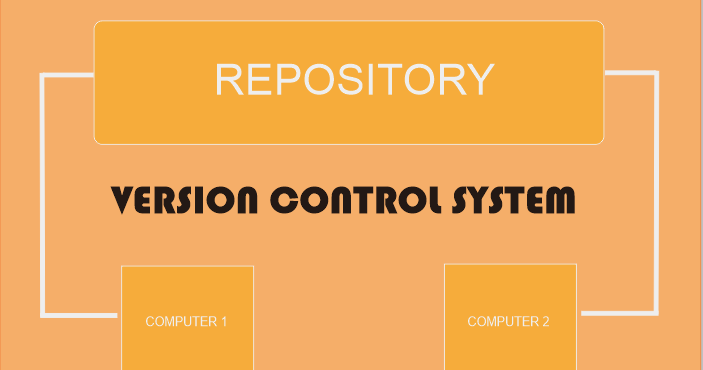
\includegraphics[scale=0.35]{figures/version-control-system/vcs}}
        \caption{Version Control System}
\end{figure}
Version Control System (VCS) adalah sebuah sistem yang melakukan source code management (SCM) )untuk mengelola perubahan di setiap dokumen, program komputer, website, dan kumpulan pemrograman lainnya.
\begin{figure}[H]
        \centerline{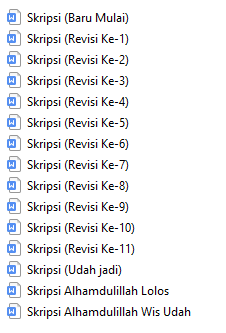
\includegraphics[scale=0.5]{figures/version-control-system/before-vcs}}
        \caption{Sebelum VCS}
\end{figure}
Lebih jelasnya kamu bisa merasakan contoh kasus yang biasa dilakukan oleh seorang mahasiswa dalam mengerjakan skripsinya. Setiap melakukan revisi, file yang telah lalu tidak akan dibuang dan akan disimpan dengan nama yang berbeda. Sedangkan yang terbaru akan disimpan dengan nama; misal “Skripsi (Revisi Ke-2)”. Kegiatan tersebut akan dilakukan secara terus menerus hingga dalam satu folder skripsi terdapat file Ms. Word dengan kuantitas yang banyak. Tujuan tersebut tidak lain adalah untuk menyimpan history pekerjaan mahasiswa. Hingga akhirnya file terakhir selesai dengan nama “Skripsi Alhamdulillah Wis Udah”. Konsep pekerjaan tersebut dianggap tidak efisien oleh banyak developer karena kapasitas penyimpanan akan membengkak. VCS disini berfungsi untuk membantu penyimpanan berupa history tanpa menyimpan file baru, yang tersimpan hanya perubahan data. Sehingga kapasitas penyimpanan file menjadi ringan.
\begin{figure}[H]
        \centerline{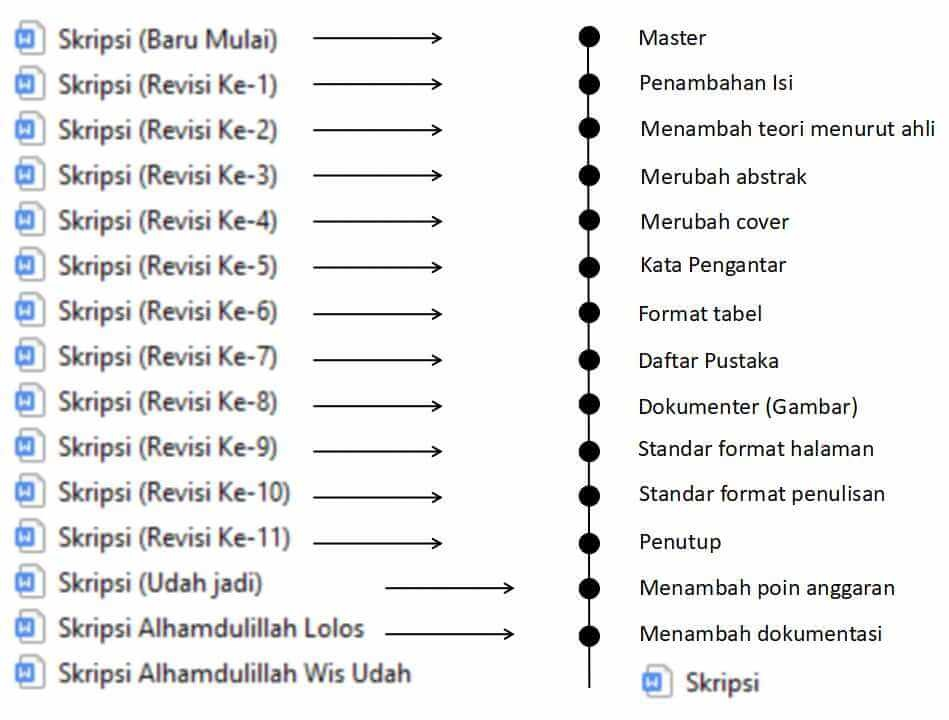
\includegraphics[scale=0.3]{figures/version-control-system/after-vcs}}
        \caption{Sesudah VCS}
\end{figure}
Seperti halnya pada gambar diatas, setiap perubahan data secara manual akan menghasilkan lebih banyak file. Sedangkan pada VCS mengusung konsep menyimpan rekaman perubahan dengan satu file saja.



\section{Git}
\begin{figure}[H]
        \centerline{
\includegraphics[scale=0.15]{figures/git/git-logo}}
        \caption{Git}
\end{figure}
Git merupakan software berbasis Version Control System (VCS) yang bertugas untuk mencatat perubahan seluruh file atau repository suatu project. Developer software biasa menggunakan Git untuk distributed revision (VCS terdistribusi), hal ini bertujuan untuk menyimpan database tidak hanya ke satu tempat. Namun semua orang yang terlibat dalam penyusunan kode dapat menyimpan database ini. Prosedur yang diterapkan ini dapat membantu antar divisi project untuk memantau dan menghubungkan (merge) antar ekstensi yang berbeda dengan mudah. Sehingga aplikasi yang dibuat oleh sebuah tim project dapat berfungsi tanpa menghubungkan secara manual. Terdapat istilah commit pada Git yang berfungsi untuk menyimpan riwayat perubahan data pada file. Melalui commit, developer dapat kembali ke source code sebelumnya dengan istilah checkout. Untuk mengoperasikan Git, kamu perlu menginstall software terlebih dahulu sehingga pekerjaan ini dapat dilakukan secara offline (tidak terkoneksi internet). Software ini juga tersedia secara gratis melalui web unduhan resminya di Git Downloading.


\section{Github}
\begin{figure}[H]
        \centerline{
\includegraphics[scale=0.45]{figures/git/github-logo}}
        \caption{Github}
\end{figure}
GitHub merupakan layanan cloud yang berguna untuk menyimpan dan mengelola sebuah project yang dinamakan repository (repo git). Cara kerja pada GitHub harus terkoneksi pada internet sehingga tidak perlu meng-install sebuah software ke dalam perangkat keras. Hal ini memberikan keringanan penyimpanan komputer yang kita gunakan karena file project tersimpan oleh cloud GitHub. Konsep kerja GitHub pada dasarnya sama dengan Git yaitu dapat menulis source code secara individu atau tim. User interface yang tersedia pada GitHub lebih menarik dan mudah dipahami oleh pengguna awal. Pekerjaan secara tim, pengguna juga bisa melihat siapa penulis kode dan tanggal berapa kode tersebut dibuat. Terdapat fitur lain pada GitHub yaitu kita dapat membaca berbagai blog dan feed yang dibuat oleh sesama pengguna. Hal ini dimanfaatkan oleh pengguna seluruh dunia untuk saling berbagi ide pemrograman dan berdiskusi dalam menyelesaikan masalah. Tentunya postingan yang ada pada GitHub berkaitan dengan pemrograman. Sehingga Github telah menjadi forum diskusi para programmer seperti halnya media sosial. Semenjak GitHub diakuisisi oleh Microsoft di tahun 2018, platform ini berkembang semakin baik dan unggul. Sehingga mayoritas programmer lebih mengenal GitHub dalam program VCS daripada pesaingnya seperti GitLab dan Atlassian BitBucket.


\section{Perbedaan Git \& Github}
Perbedaan antara Git dan GitHub sangat unik dan memiliki keunggulan masing-masing. Berikut ini perbedaan dari kedua platform tersebut.
\begin{center}
\begin{tabular}{ | m{6cm} | m{6cm} | }
\hline
Git & Github \\
\hline
1. Meng-install software di penyimpanan lokal & 1. Host melalui layanan cloud \\
\hline
2. Dikelola oleh The Linux Foundation & 2. Diakuisisi oleh Microsoft pada 2018 \\
\hline
3. Berfokus pada version control dan code sharing & 3. Berfokus pada source code hosting terpusat \\
\hline
4. Akses secara offline & 4. Akses secara online \\
\hline
5. Tidak menggunakan fitur user management & 5. Menggunakan user management \\
\hline
6. Menyediakan desktop interface bernama “Git GUI” & 6. Menggunakan nama desktop interface “GitHub Desktop” \\
\hline
7. Bersaing dengan Mercurial, Subversion, IBM, Rational Team, Concert, dan ClearCase & 7. Bersaing dengan GitLab dan Atlassian BitBucket \\
\hline
8. Open sourced licensed & 8. Pilihan bagi pengguna gratis dan pengguna berbayar \\
\hline
\end{tabular}
\end{center}


\section{Tutorial Membuat Akun Github}
Disini saya akan membahas bagaimana cara mudah membuat akun Github beserta gambar.
\begin{enumerate}
\item kunjungi website \url{https://github.com}, lalu klik sign up untuk mendaftar
\begin{figure}[H]
        \centerline{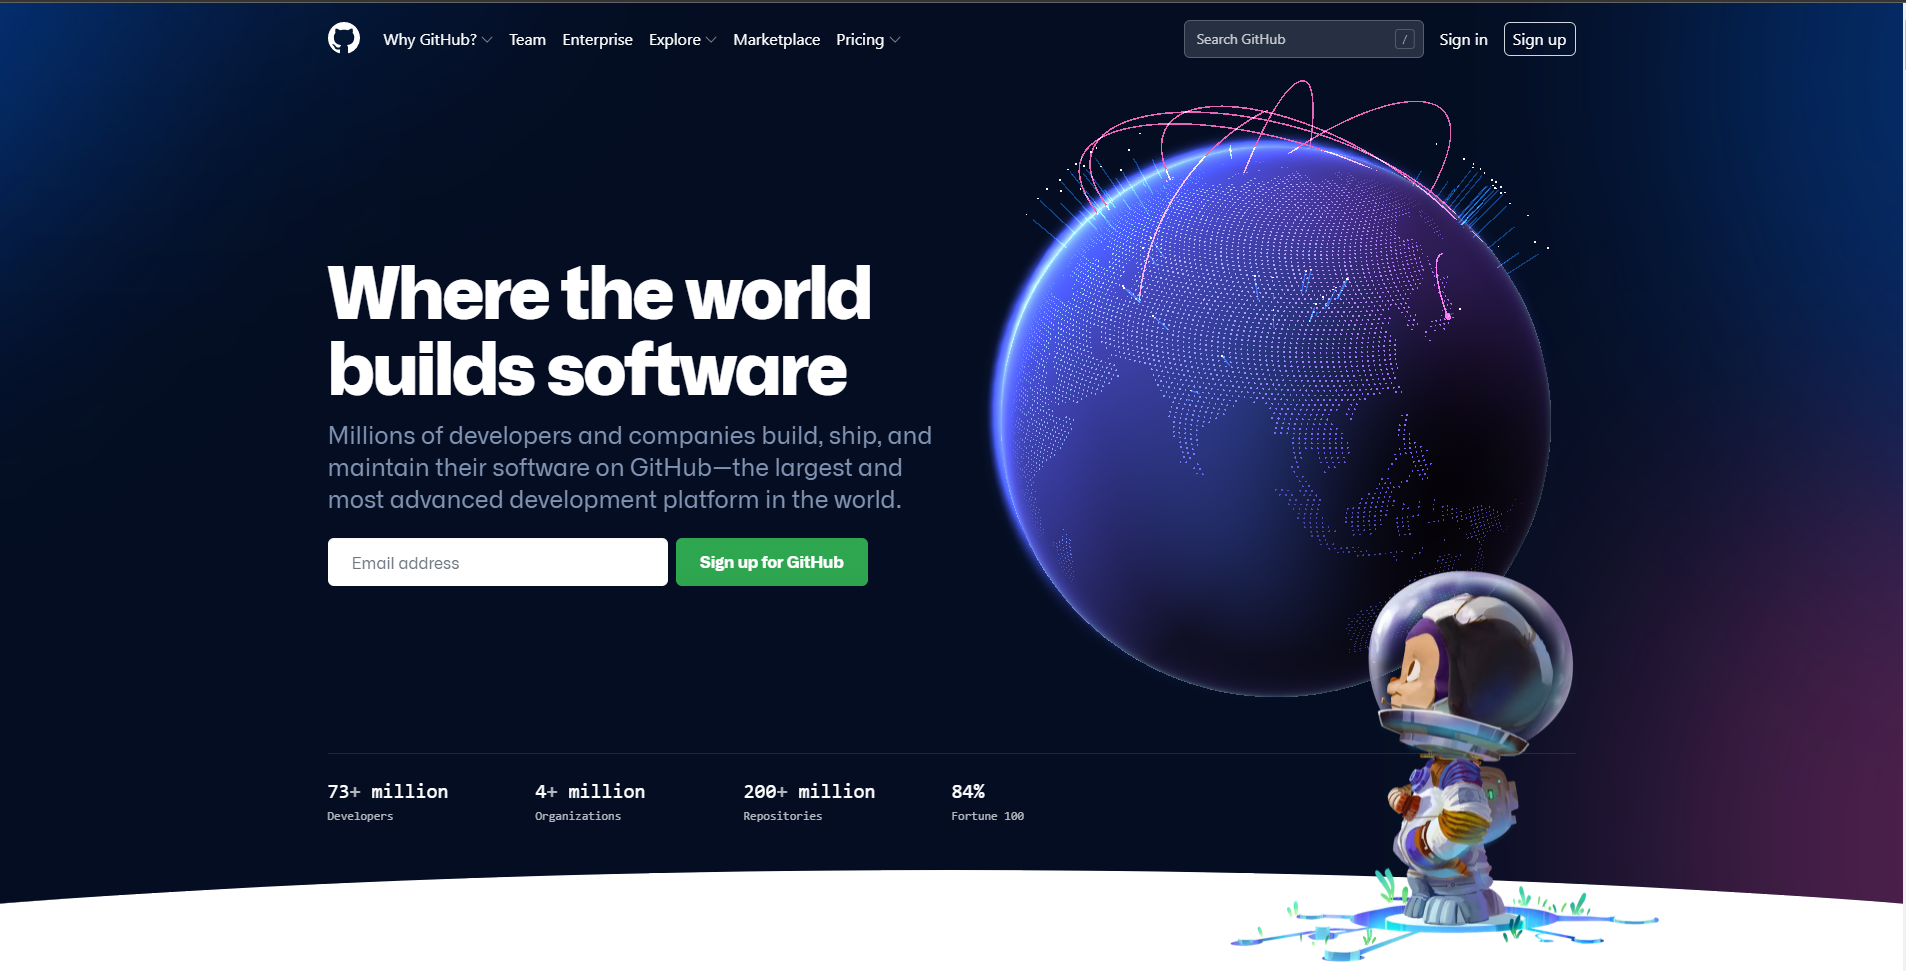
\includegraphics[scale=0.25]{figures/buat-akun-github/step1}}
        \caption{Tutorial Akun Github: Step 1}
\end{figure}
\item lalu akan dialihkan kehalaman pendaftaran, isikan email yang aktif, lalu klik Enter
\begin{figure}[H]
        \centerline{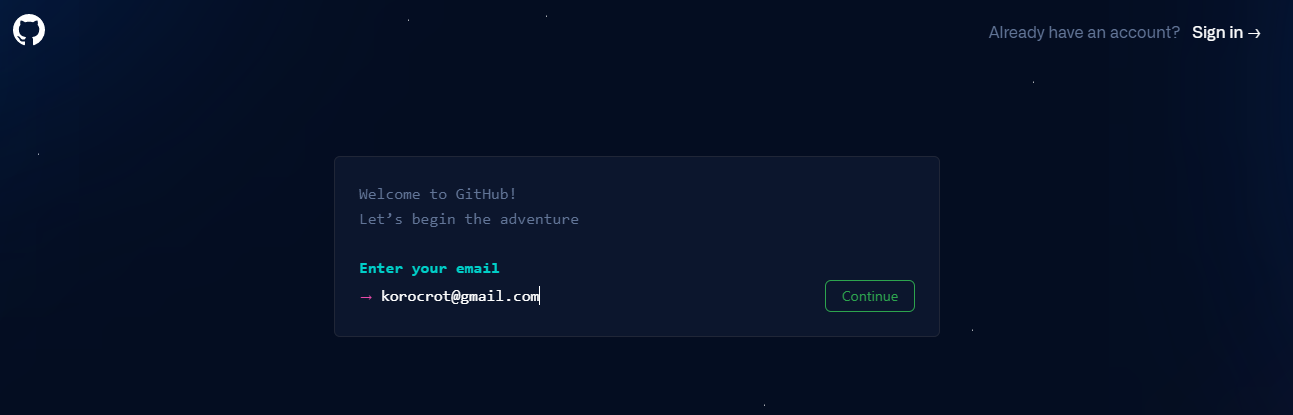
\includegraphics[scale=0.35]{figures/buat-akun-github/step2}}
        \caption{Tutorial Akun Github: Step 2}
\end{figure}
\item lalu masukkan password yang dengan kombinasi yang direkomendasikan oleh Github
\begin{figure}[H]
        \centerline{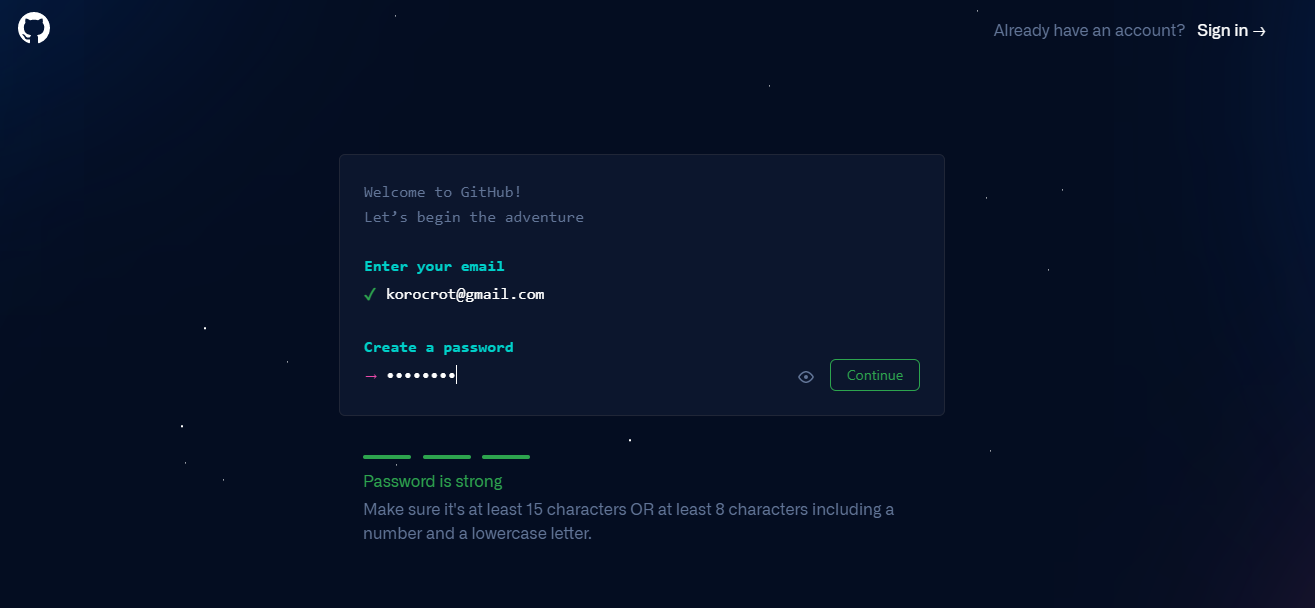
\includegraphics[scale=0.35]{figures/buat-akun-github/step3}}
        \caption{Tutorial Akun Github: Step 3}
\end{figure}
\item masukkan username yang unik, jika username tidak tersedia coba beberapa kombinasi seperti angka dan huruf
\begin{figure}[H]
        \centerline{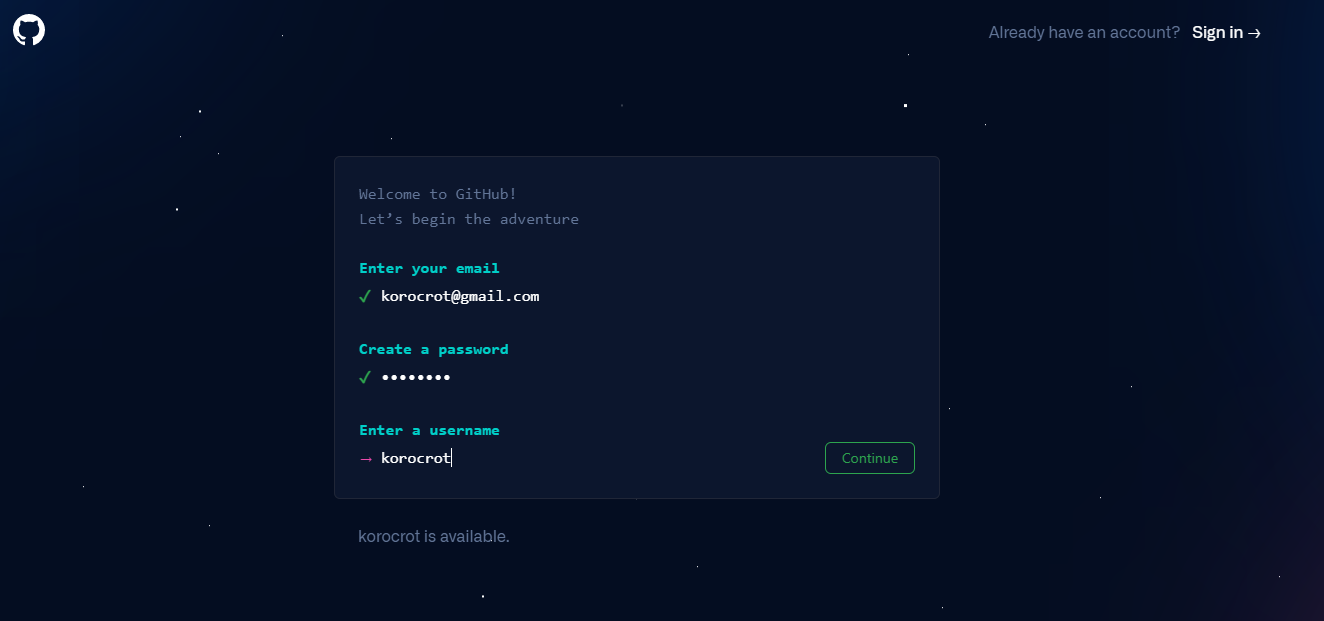
\includegraphics[scale=0.35]{figures/buat-akun-github/step4}}
        \caption{Tutorial Akun Github: Step 4}
\end{figure}
\item lalu setelah itu akan muncul penawaran dari Github untuk notifikasi product dan announcement, saya disini memilih "n"
\begin{figure}[H]
        \centerline{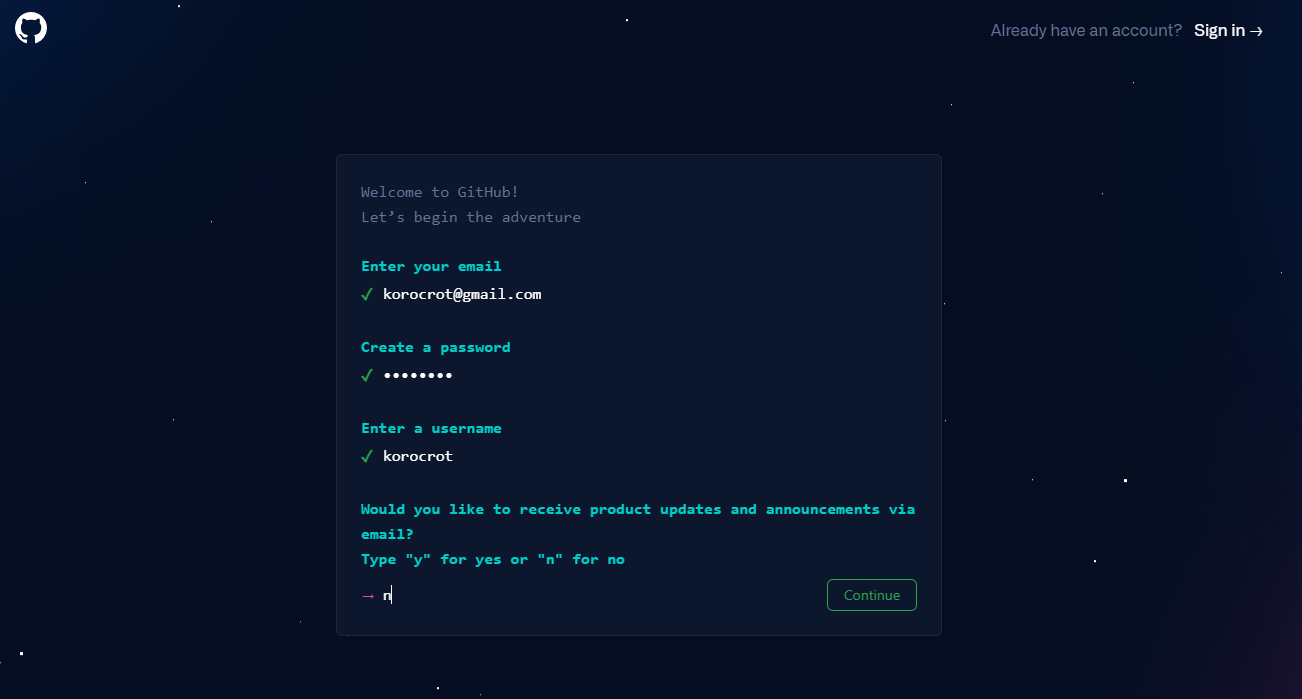
\includegraphics[scale=0.35]{figures/buat-akun-github/step5}}
        \caption{Tutorial Akun Github: Step 5}
\end{figure}
\item setelah itu akan diminta untuk menyelesaikan puzzle untuk verifikasi bahwa yang mendaftar adalah manusia, selesaikan puzze berdasarkan perintah yang diberikan
\begin{figure}[H]
        \centerline{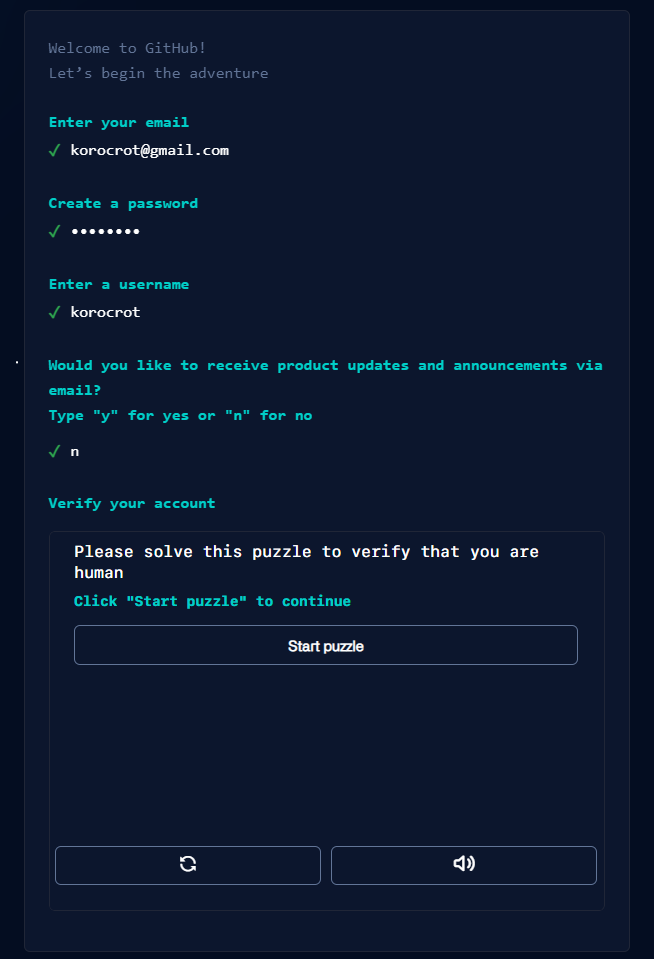
\includegraphics[scale=0.35]{figures/buat-akun-github/step6}}
        \caption{Tutorial Akun Github: Step 6}
\end{figure}
\item jika berhasil bisa langsung klik \textbf{Create account}
\begin{figure}[H]
        \centerline{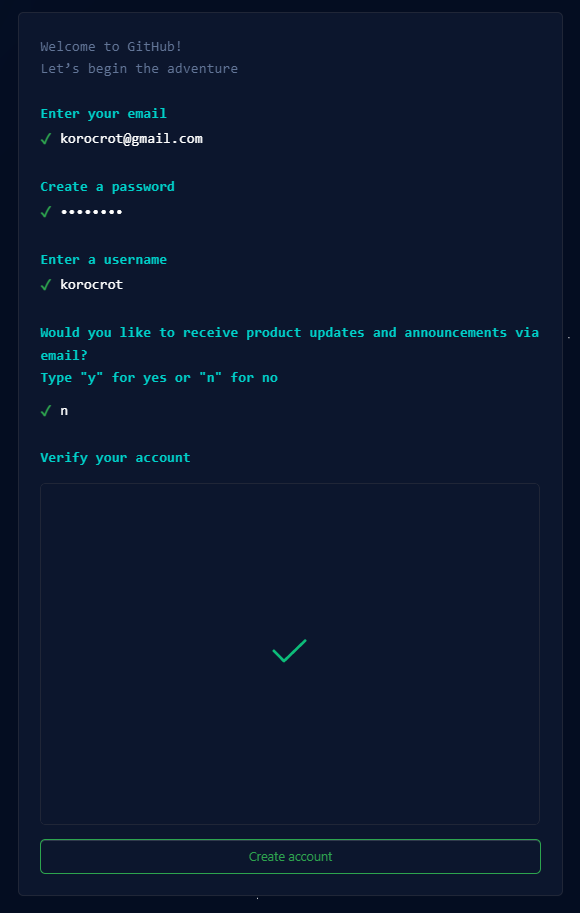
\includegraphics[scale=0.35]{figures/buat-akun-github/step7}}
        \caption{Tutorial Akun Github: Step 7}
\end{figure}
\item lalu Github akan mengirimkan kode verifikasi ke email yang didaftarkan
\begin{figure}[H]
        \centerline{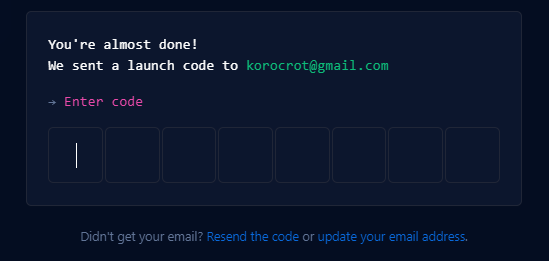
\includegraphics[scale=0.35]{figures/buat-akun-github/step8}}
        \caption{Tutorial Akun Github: Step 8}
\end{figure}
\item copy dan paste code yang ada di email ke kotak \textbf{Enter code} git halaman github, Note: jangan menutup tab Github
\begin{figure}[H]
        \centerline{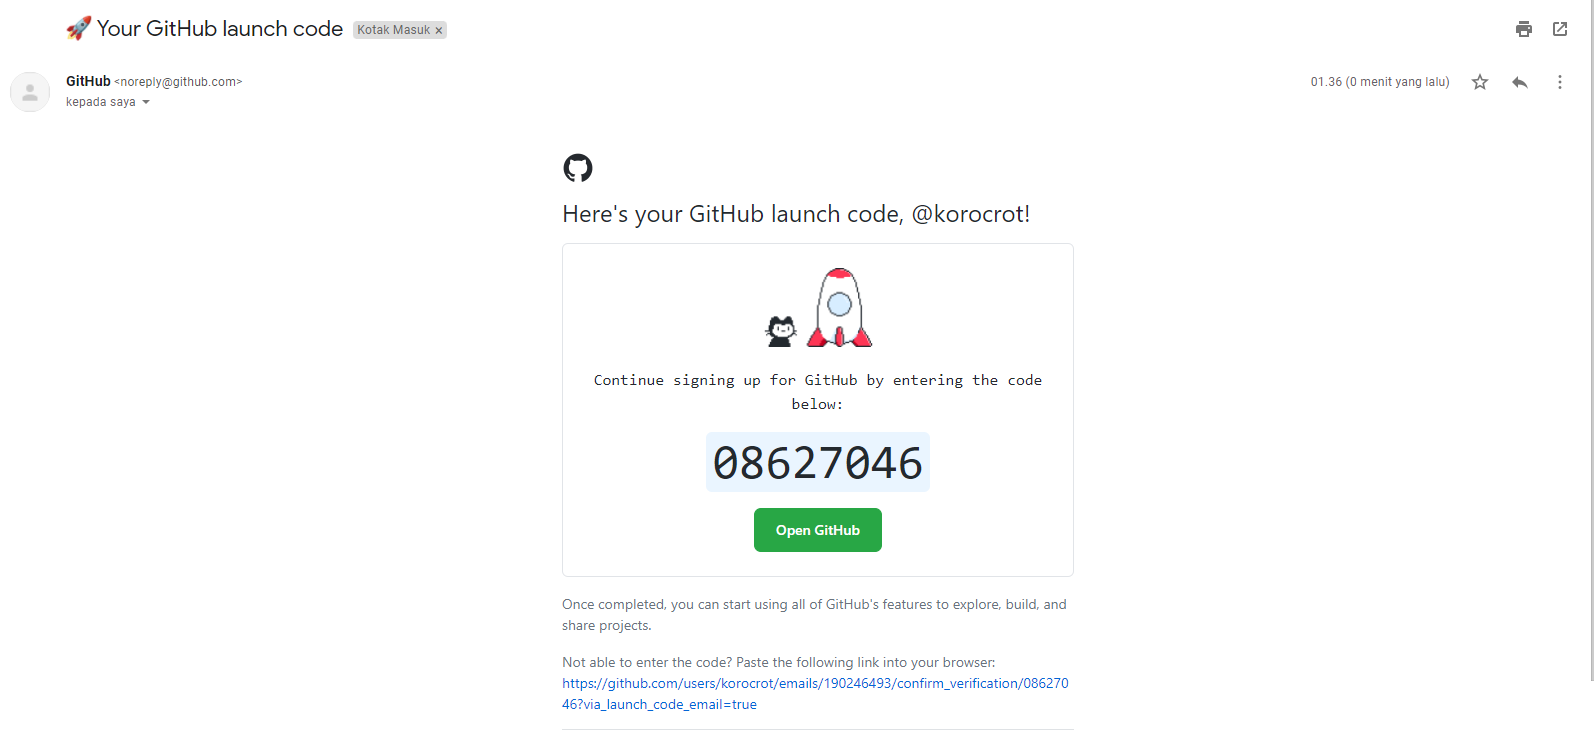
\includegraphics[scale=0.35]{figures/buat-akun-github/step9}}
        \caption{Tutorial Akun Github: Step 9}
\end{figure}
\item jika kode yang dimasukkan benar maka kamu akan dialihkan ke halaman dashboard github
\begin{figure}[H]
        \centerline{\includegraphics[scale=0.25]{figures/buat-akun-github/step10}}
        \caption{Tutorial Akun Github: Step 10}
\end{figure}
\end{enumerate}


\section{Tutorial Install Git}
Disini saya akan membahas bagaimana cara mudah menginstall Git pada Windows 10 \& Linux beserta gambar.

\subsection{Windows 10}
\begin{enumerate}
\item kunjungi website git-scm \url{https://git-scm.com/}
\item lalu klik menu \textbf{Download}
\item akan muncul seperti gambar dibawah, lalu klik \textbf{Download for Windows}
\begin{figure}[H]
        \centerline{\includegraphics[scale=0.3]{figures/instalasi-git-scm-windows/step1}}
        \caption{Tutorial Install Git-scm: Step 1}
\end{figure}
\item setelah berhasil download, klik (2x) dan akan muncul menu seperti dibawah ini, klik next
\begin{figure}[H]
        \centerline{\includegraphics[scale=0.5]{figures/instalasi-git-scm-windows/step2}}
        \caption{Tutorial Install Git-scm: Step 2}
\end{figure}
\item klik next
\begin{figure}[H]
        \centerline{\includegraphics[scale=0.5]{figures/instalasi-git-scm-windows/step3}}
        \caption{Tutorial Install Git-scm: Step 3}
\end{figure}
\item klik next
\begin{figure}[H]
        \centerline{\includegraphics[scale=0.5]{figures/instalasi-git-scm-windows/step4}}
        \caption{Tutorial Install Git-scm: Step 4}
\end{figure}
\item klik install
\begin{figure}[H]
        \centerline{\includegraphics[scale=0.5]{figures/instalasi-git-scm-windows/step5}}
        \caption{Tutorial Install Git-scm: Step 5}
\end{figure}
\item tunggu instalasi hingga selesai
\begin{figure}[H]
        \centerline{\includegraphics[scale=0.5]{figures/instalasi-git-scm-windows/step6}}
        \caption{Tutorial Install Git-scm: Step 6}
\end{figure}
\item klik finish
\begin{figure}[H]
        \centerline{\includegraphics[scale=0.5]{figures/instalasi-git-scm-windows/step7}}
        \caption{Tutorial Install Git-scm: Step 7}
\end{figure}
\end{enumerate}

\subsection{Linux}
untuk instalasi linux bisa dibilang cukup mudah tidak serumit windows, berikut caranya.
\begin{enumerate}
\item buka terminal dan ketikkan \textbf{sudo apt-get install git -y} seperti gambar dibawah ini, lalu tekan Enter
\begin{figure}[H]
        \centerline{\includegraphics[scale=0.5]{figures/instalasi-git-linux/step1}}
        \caption{Tutorial Install Git Linux: Step 1}
\end{figure}
\item tunggu hingga instalasi selesai seperti gambar dibawah ini
\begin{figure}[H]
        \centerline{\includegraphics[scale=0.5]{figures/instalasi-git-linux/step2}}
        \caption{Tutorial Install Git Linux: Step 2}
\end{figure}
\end{enumerate}


\section{Generate SSH Key}
Pada section ini saya akan memberikan tutorial cara generate SSH key yang nantinya SSH key tersebut digunakan untuk mengakses website Github.
\begin{enumerate}
\item pertama buka git bash terminal, lalu ketikkan perintah dibawah, lalu tekan Enter
\begin{lstlisting}
ssh-keygen -t rsa -b 4096 -C "email@anda.com"
\end{lstlisting}
\begin{figure}[H]
        \centerline{\includegraphics[scale=0.5]{figures/generate-ssh-key/step1}}
        \caption{Tutorial Generate SSH Key: Step 1}
\end{figure}
\item setelah itu akan muncul informasi isian seperti gambar dibawah ini, tekan Enter saja
\begin{figure}[H]
        \centerline{\includegraphics[scale=0.5]{figures/generate-ssh-key/step2}}
        \caption{Tutorial Generate SSH Key: Step 2}
\end{figure}
\item akan muncul lagi isian berikutnya, tekan Enter saja
\begin{figure}[H]
        \centerline{\includegraphics[scale=0.5]{figures/generate-ssh-key/step3}}
        \caption{Tutorial Generate SSH Key: Step 3}
\end{figure}
\item akan muncul lagi isian, tekan Enter saja
\begin{figure}[H]
        \centerline{\includegraphics[scale=0.5]{figures/generate-ssh-key/step4}}
        \caption{Tutorial Generate SSH Key: Step 4}
\end{figure}
\item jika sudah selesai akan muncul seperti gambar dibawah ini
\begin{figure}[H]
        \centerline{\includegraphics[scale=0.5]{figures/generate-ssh-key/step5}}
        \caption{Tutorial Generate SSH Key: Step 5}
\end{figure}
\end{enumerate}


\section{Memasang SSH Key di Github}
Section ini akan memberikan tutorial bagaimana memasang SSH Key di Github agar komputer bisa terkoneksi dengan akun Github
\begin{enumerate}
\item kunjungi \url{https://github.com} dan login menggunakan akun yang sudah didaftarkan sebelumnya
\begin{figure}[H]
        \centerline{\includegraphics[scale=0.5]{figures/memasang-ssh-key/step1}}
        \caption{Tutorial Memasang SSH Key: Step 1}
\end{figure}
\item jika sudah login klik profile dan klik settings
\begin{figure}[H]
        \centerline{\includegraphics[scale=0.5]{figures/memasang-ssh-key/step2}}
        \caption{Tutorial Memasang SSH Key: Step 2}
\end{figure}
\item setelah itu klik SSH dan GPG Keys
\begin{figure}[H]
        \centerline{\includegraphics[scale=0.5]{figures/memasang-ssh-key/step3}}
        \caption{Tutorial Memasang SSH Key: Step 3}
\end{figure}
\item lalu klik new ssh keys
\begin{figure}[H]
        \centerline{\includegraphics[scale=0.5]{figures/memasang-ssh-key/step4}}
        \caption{Tutorial Memasang SSH Key: Step 4}
\end{figure}
\item lalu buka git bash anda dan ketikkan perintah dibawah, lalu enter, dan copy output yang dikeluarkan
\begin{lstlisting}
cat .ssh/id_rsa.pub
\end{lstlisting}
\begin{figure}[H]
        \centerline{\includegraphics[scale=0.5]{figures/memasang-ssh-key/step5}}
        \caption{Tutorial Memasang SSH Key: Step 5}
\end{figure}
\item setelah itu isi title dengan isian bebas, lalu paste yang sudah dicopy di bagian form bawah seperti gambar dibawah ini, lalu klik add ssh key
\begin{figure}[H]
        \centerline{\includegraphics[scale=0.5]{figures/memasang-ssh-key/step6}}
        \caption{Tutorial Memasang SSH Key: Step 6}
\end{figure}
\item jika tampilan seperti dibawah ini maka tahap memasang ssh key sudah selesai
\begin{figure}[H]
        \centerline{\includegraphics[scale=0.5]{figures/memasang-ssh-key/step7}}
        \caption{Tutorial Memasang SSH Key: Step 7}
\end{figure}
\end{enumerate}


\chapter{Algoritma}
\section{Algoritma}
\begin{figure}[H]
        \centerline{\includegraphics[scale=0.5]{figures/algoritma-kompleksitas/algoritma}}
        \caption{Algoritma}
\end{figure}
sebelum jauh kita bahas tentang yang lainnya, mari kita bahas apa itu Algoritma:

\textit{Algoritma adalah sebuah proses atau seperangkat aturan yang harus diikuti dalam operasi pemecahan masalah}
Sederhananya, algoritma adalah serangkaian proses yang dilakukan secara berurutan untuk menyelesaikan sebuah permasalahan. Algoritma bisa bermacam-macam tergantung kepada siapa yang membuat algoritma tersebut. Namun permasalahannya adalah algoritma mana yang lebih efektif dan efisien? Algoritma sangat banyak digunakan dikehidupan sehari-hari, contohnya adalah bagaimana anda memasak air, bagaimana memasak mie instan, bagaimana menyalakan mesin motor, dan lain sebagainya yang dimana aktivitas tersebut terdapat proses alur yang jika kita ikuti maka akan mencapai suatu tujuan yang ingin kita capai, seperti ingin menyalakan motor contoh yang saya ketahui adalah sebagai berikut,
\begin{enumerate}
\item ambil kunci motor
\item masukkan kunci motor pada \textbf{main switch}
\item putar hingga ke arah on
\item lalu tekan tombol starter pada motor
\item motor menyala
\end{enumerate}

Kita bisa sebut algoritma diatas adalah algoritma K untuk menyalakan sebuah motor, lalu beberapa tahun kemudian ada algoritma baru yaitu algoritma KL dimana algoritma ini bisa menyelesaikan masalah diatas dengan lebih cepat, kita tidak diperlukan lagi untuk memasukkan kunci motor pada \textbf{main switch}, ketika anda sudah dekat dengan motor cukup putar alat yang ada di main switch hingga on dan starter motor, kita contohnya dibawah ini
\begin{enumerate}
\item ambil kunci motor
\item putar tuas main switch ke arah on
\item tekan tombol starter pada motor
\item motor menyala
\end{enumerate}

Jika kita bandingkan dua algoritma diatas K dan KL sama-sama menyelesaikan masalah yaitu bagaimana motor bisa menyala, akan tetapi ada 2 perbedaan yaitu di Time dan Space, mari kita lihat perbedaannya, dari segi langkah algoritma K memiliki 5 langkah agar motor bisa menyala, akan tetapi algoritma KL hanya memiliki 4 langkah, jika kita berikan 1 langkah = 1 detik maka algoritma KL bisa menghemat waktu hingga 1 detik. Lalu kita bandingkan dengan Space, algoritma KL ternyata untuk bisa mempercepat 1 detik maka dibutuhkan berat, material, teknologi, dan lainnya lebih tinggi 2x dari algoritma K. Tentunya 2 algoritma bisa menjadi solusi terbaik bagi beberapa masalah yang dihadapi.

\section{Cases}
Untuk memenuhi beberapa petunjuk, ada 3 case untuk merepresentasikan suatu algoritma untuk mencapai atau menyelesaiakn masalahnya.

\subsection{Worst Case}
Worst case atau bisa kita terjemahkan ke Bahasa Indonesia adalah kasus terburuk merupakan definisi dari sebuah \textit{class} yang menunjukkan runtime terburuk dari sebuah algoritma. Perancang algoritma biasanya akan memberikan nilai input untuk mencegah sebuah algoritma berjalan secara efisien untuk mengetahui kasus terburuk dari sebuah algoritma.

Contoh kasusnya adalah untuk setiap nilai \textit{n} tertentu, runtime yang dilakukan oleh suatu algoritma atau program dapat bervariasi terhadap nilai n. Untuk program yang diberikan nilai n, maka waktu eksekusi terburuk adalah waktu eksekusi maksimum dimana maksimum diambil dari instance berukuran n. Worst case adalah kasus dimana algoritma sering dijumpai dan sangat mudah untuk dianalisa. Worst case juga bisa menjadi penjelasan mengapa sebuah program berjalan dengan sangat lambat dalam situasi apapun.

\subsection{Average Case}
Average case atau kasus rata-rata adalah definisi dari sebuah perilaku algoritma yang dimana runtime sebuah algoritma akan membutuhkan lebih banyak waktu untuk diselesaikan untuk beberapa kasus tertentu, sebagian besar tidak. Ukuran ini menggambarkan ekspektasi dari pengguna algoritma.

Kasus rata-rata sering dijumpai oleh pengguna algoritma dikarenakan algoritma ini akan menyelesaikan sebuah kasus dalam runtime yang rata-rata, tidak terlalu lama, tidak juga sangat cepat.

\subsection{Best Case}
Best case adalah definisi masalah algoritme yang menunjujkkan runtime terbaiknya pada suatu kasus. Algoritma yang termasuk dalam best case adalah algoritma yang bekerja paling sedikit. Akan tetapi pada kenyataannya algoritma dengan best case sangat jarang ditemukan.

Mengetahui kasus terbaik untuk suatu algoritma sangat berguna meskipun situasinya jarang terjadi dalam praktik secara langsung. Dalam banyak kasus, hal ini memberikan informasi tentang keadaan optimal dari suatu algoritma. Misalnya, best case untuk Counting Search adalah ketika mencari nilai yang diinginkan contohnya adalah \textit{v}. Counting Search akan menghitung berapa kali \textit{v} muncul. Jika hitungan yang dihitung adalah nol, maka item tersebut tidak ditemukan, sehingga algoritma akan mengembalikan nilai \textit{false} jika ditemukan maka algoritma akan mengembalikan nilai \textit{true}. Ada beberapa perhatian yang harus dianalisis yaitu Counting Search akan menelusuri seluruh daftar, oleh karena itu meskipun perilaku kasus terburuknya adalah O(n) dilain sisi kasus terbaiknya atau best case tetap O(n).

\chapter{Hash Map}
\section{Hash Map}
\begin{figure}[H]
        \centerline{\includegraphics[scale=0.5]{figures/hash-map/hash-function}}
        \caption{Hash Map}
\end{figure}
Hash Map merupakan struktur data yang memiliki indeks. Hash map menggunakan fungsi hash untuk menghitung indeks dengan key ke dalam buckets atau slot. Nilainya dipetakan ke buckets dengan indeks yang sesuai dan key yang unik dan tidak berubah. Kita ibaratkan has map dengan sebuah lemari yang memiliki laci dengan label untuk barang-barang yang disimpan di dalamnya. Misalnya, menyimpan infoemasi pengguna dan email sebagai keynya, dan kita dapat memetakan nilai yang terkait dengan pengguna tersebut seperti nama depan, nama belakang, dll ke dalam buckets.

Hashmap adalah tipe struktur data yang memetakan kunci ke pasangan nilainya (menerapkan tipe data array abstrak). Ini pada dasarnya menggunakan fungsi yang menghitung nilai indeks yang pada gilirannya menyimpan elemen yang akan dicari, dimasukkan, dihapus, dll. Ini membuatnya mudah dan cepat untuk mengakses data. Secara umum, tabel hash menyimpan pasangan key value dan key tersebut dihasilkan menggunakan fungsi hash. Jadi fungsi pencarian dan penyisipan elemen data menjadi lebih cepat karena nilai key itu sendiri menjadi indeks yang menyimpan data.

Fungsi hash adalah inti dari implementasi hash map. Fungsi hash mengambil kunci dan menerjemahkannya ke indeks buckets di daftar buckets. Hashing yang ideal harus menghasilkan indeks yang berbeda untuk setiap key. Namun, hal ini bisa menyebabkan collisions. Saat hashing memberikan indeks yang ada, kita cukup menggunakan buckets untuk beberapa nilai dengan appending list atau dengan rehashing.

Dalam python, dict merupakan contoh dari hash map. Kita akan melihat implementasi hash map dari awal untuk mempelajari cara membangun dan menyesuaikan struktur data tersebut agar dapat mengoptimalkan pencarian.
Desain hash map akan mencakup fungsi-fungsi berikut:
\begin{enumerate}

\item set\_val(key, value): Menyisipkan pasangan key-value ke dalam peta hash. Jika nilai sudah ada di peta hash, perbarui nilainya.

\item get\_val(key): Mengembalikan nilai di mana key yang ditentukan dimapping, atau “Tidak ada catatan yang ditemukan” jika map ini tidak berisi pemetaan untuk key tersebut.

\item delete\_val(key): Menghapus pemetaan untuk key tertentu jika hash map berisi pemetaan untuk key tersebut.
\end{enumerate}
Berikut contoh implementasi hash map:
\begin{lstlisting}[language=Python, caption=Implementasi Hash Map]
class HashTable:

	# Create empty bucket list of given size
	def __init__(self, size):
		self.size = size
		self.hash_table = self.create_buckets()

	def create_buckets(self):
		return [[] for _ in range(self.size)]

	# Insert values into hash map
	def set_val(self, key, val):
		
		# Get the index from the key
		# using hash function
		hashed_key = hash(key) % self.size
		
		# Get the bucket corresponding to index
		bucket = self.hash_table[hashed_key]

		found_key = False
		for index, record in enumerate(bucket):
			record_key, record_val = record
			
			# check if the bucket has same key as
			# the key to be inserted
			if record_key == key:
				found_key = True
				break

		# If the bucket has same key as the key to be inserted,
		# Update the key value
		# Otherwise append the new key-value pair to the bucket
		if found_key:
			bucket[index] = (key, val)
		else:
			bucket.append((key, val))

	# Return searched value with specific key
	def get_val(self, key):
		
		# Get the index from the key using
		# hash function
		hashed_key = hash(key) % self.size
		
		# Get the bucket corresponding to index
		bucket = self.hash_table[hashed_key]

		found_key = False
		for index, record in enumerate(bucket):
			record_key, record_val = record
			
			# check if the bucket has same key as
			# the key being searched
			if record_key == key:
				found_key = True
				break

		# If the bucket has same key as the key being searched,
		# Return the value found
		# Otherwise indicate there was no record found
		if found_key:
			return record_val
		else:
			return "No record found"

	# Remove a value with specific key
	def delete_val(self, key):
		
		# Get the index from the key using
		# hash function
		hashed_key = hash(key) % self.size
		
		# Get the bucket corresponding to index
		bucket = self.hash_table[hashed_key]

		found_key = False
		for index, record in enumerate(bucket):
			record_key, record_val = record
			
			# check if the bucket has same key as
			# the key to be deleted
			if record_key == key:
				found_key = True
				break
		if found_key:
			bucket.pop(index)
		return

	# To print the items of hash map
	def __str__(self):
		return "".join(str(item) for item in self.hash_table)


hash_table = HashTable(50)

# insert some values
hash_table.set_val('gfg@example.com', 'some value')
print(hash_table)
print()

hash_table.set_val('portal@example.com', 'some other value')
print(hash_table)
print()

# search/access a record with key
print(hash_table.get_val('portal@example.com'))
print()

# delete or remove a value
hash_table.delete_val('portal@example.com')
print(hash_table)

\end{lstlisting}

\section{Tabel Hash vs Hashmap: Perbedaan antara Tabel Hash dan Hashmap dengan Python}
Berikut perbedaan antara Hash Table dengan Hash Map.
\begin{table}[H]
\begin{tabular}{ll}
Hash Table                                               & Hash Map                               \\
Disinkronkan                                             & Tidak Disinkronkan                     \\
Cepat                                                    & Lambat                                 \\
Mengizinkan satu kunci nol dan lebih dari satu nilai nol & Tidak mengizinkan kunci atau nilai nol
\end{tabular}
\end{table}

\section{Membuat Dictionary}
Dictionary dapat dibuat dengan dua cara:
\begin{enumerate}
\item Menggunakan kurung kurawal ({})
Berikut contoh pembuatan dictionary menggunakan kurung kurawal.
\begin{lstlisting}[language=Python, caption=Dict dengan Kurung Kurawal]
my_dict={'Dave' : '001' , 'Ava': '002' , 'Joe': '003'}
print(my_dict)
type(my_dict)
\end{lstlisting}
\item menggunakan fungsi dict()
Python memiliki fungsi bawaan dict() yang dapat digunakan untuk membuat dictionary, berikut contoh penggunaannya:
\begin{lstlisting}[language=Python, caption=Dict dengan Kurung Kurawal]
new_dict=dict()
print(new_dict)
type(new_dict)
\end{lstlisting}
Dalam contoh di atas, dictionary kosong dibuat karena tidak ada pasangan key-value yang diberikan sebagai parameter ke fungsi dict(). Jika teman-teman ingin menambahkan nilai, teman-teman dapat melakukan hal berikut:
\begin{lstlisting}[language=Python, caption=Dict dengan Kurung Kurawal]
new_dict=dict(Dave = '001' , Ava= '002' , Joe= '003')
print(new_dict)
type(new_dict)
\end{lstlisting}
\end{enumerate}

\section{Membuat Nested Dictionary}
Nested Dictionary merupakan dictionary yang terletak di dalam dictionary. Berikut contoh nested dictionary:

\begin{lstlisting}[language=Python, caption=Nested Dict]
emp_details = {'Employee': {'Dave': {'ID': '001',
                                     'Salary': 2000,
                                     'Designation':'Python Developer'},
                            'Ava': {'ID':'002',
                                    'Salary': 2300,
                                    'Designation': 'Java Developer'},
                            'Joe': {'ID': '003',
                                    'Salary': 1843,
                                    'Designation': 'Hadoop Developer'}}}
\end{lstlisting}

\section{Melakukan Operasi pada Hash Table menggunakan Dictionary}
Berikut beberapa operasi yang dapat dilakukan pada hash table dalam python melalui dictionary:
\begin{enumerate}
\item Mengakses Nilai
Nilai dictionary bisa diakses dengan berbagai cara seperti berikut:
\begin{enumerate}
\item Menggunakan nilai key
Nilai dictionary dapat diakses menggunakan nilai key sebagai berikut:
\begin{lstlisting}[language=Python, caption=Dict dengan nilai key]
my_dict={'Dave' : '001' , 'Ava': '002' , 'Joe': '003'}
my_dict['Dave']
\end{lstlisting}
Outputnya yaitu 001
\item Menggunakan fungsi
Ada beberapa fungsi bawaan yang dapat digunakan seperti get(), keys(), values(), dll.
\begin{lstlisting}[language=Python, caption=Dict with function]
my_dict={'Dave' : '001' , 'Ava': '002' , 'Joe': '003'}
print(my_dict.keys())
print(my_dict.values())
print(my_dict.get('Dave'))
\end{lstlisting}
Output sebagai berikut:
\begin{lstlisting}
dict_keys(['Dave', 'Ava', 'Joe'])
dict_values(['001', '002', '003'])
001
\end{lstlisting}
\item Menerapkan for loop
Perulangan for memungkinkan Anda mengakses pasangan nilai key dictionary dengan mudah dengan mengulanginya. Sebagai contoh:
\begin{lstlisting}[language=Python, caption=Dict For Loop]
my_dict={'Dave' : '001' , 'Ava': '002' , 'Joe': '003'}
print("All keys")
for x in my_dict:
    print(x)       #prints the keys
print("All values")
for x in my_dict.values():
    print(x)       #prints values
print("All keys and values")
for x,y in my_dict.items():
    print(x, ":" , y)       #prints keys and values
\end{lstlisting}
Output:
\begin{lstlisting}
Semua kunci
Dave
Ava
Joe
Semua nilai
001
002
003
Semua kunci dan nilai
Dave : 001
Ava : 002
Joe : 003
\end{lstlisting}
\end{enumerate}
\item Memperbarui Nilai
Dictionary adalah tipe data yang bisa berubah dan oleh karena itu, teman-teman dapat memperbaruinya jika diperlukan. Misalnya, jika saya ingin mengubah ID karyawan bernama Dave dari '001' menjadi '004' dan jika saya ingin menambahkan pasangan nilai kunci lain ke kamus saya, saya dapat melakukan hal berikut:
\begin{lstlisting}[language=Python, caption=Dict For Loop]
my_dict={'Dave' : '001' , 'Ava': '002' , 'Joe': '003'}
my_dict['Dave'] = '004'   #Updating the value of Dave
my_dict['Chris'] = '005'  #adding a key-value pair
print(my_dict)
\end{lstlisting}
Output:
\begin{lstlisting}
{'Dave': '004', 'Ava': '002', 'Joe': '003', 'Chris': '005'}
\end{lstlisting}
\item Menghapus Elemen
Ada sejumlah fungsi yang memungkinkan Anda untuk menghapus item dari dictionary seperti del(), pop(), popitem(), clear(), dll. Misalnya:
\begin{lstlisting}[language=Python, caption=Dict For Loop]
my_dict={'Dave': '004', 'Ava': '002', 'Joe': '003', 'Chris': '005'}
del my_dict['Dave']  #removes key-value pair of 'Dave'
my_dict.pop('Ava')   #removes the value of 'Ava'
my_dict.popitem()    #removes the last inserted item
print(my_dict)
\end{lstlisting}
Output: {'Joe': '003'}. Output di atas menunjukkan bahwa semua elemen kecuali 'Joe: 003' telah dihapus dari kamus menggunakan berbagai fungsi.
\end{enumerate}

\section{Mengubah Dictionary menjadi Kerangka Data}
Seperti yang telah teman-teman lihat sebelumnya, saya telah membuat nested dictionary yang berisi nama karyawan dan detailnya dipetakan ke sana. Sekarang untuk membuat tabel yang jelas dari itu, saya akan menggunakan library pandas untuk meletakkan semuanya sebagai kerangka data.
\begin{lstlisting}[language=Python, caption=Mengubah Dictionary menjadi Kerangka Data]
import pandas as pd
emp_details = {'Employee': {'Dave': {'ID': '001',
                                     'Salary': 2000,
                                     'Designation':'Python Developer'},
                            'Ava': {'ID':'002',
                                    'Salary': 2300,
                                    'Designation': 'Java Developer'},
                            'Joe': {'ID': '003',
                                    'Salary': 1843,
                                    'Designation': 'Hadoop Developer'}}}
df=pd.DataFrame(emp_details['Employee'])
print(df)
\end{lstlisting}

Output:
\begin{figure}[H]
    \centering
    \includegraphics[scale=0.3]{figures/hash-map/output}
    \caption{\textit{Output Dictionary}}
    \label{colab6}
\end{figure}

\chapter{Hash Tables}
\section{Hash Table}
\begin{figure}[H]
        \centerline{\includegraphics[scale=0.5]{figures/hash-tables/hash-function}}
        \caption{Hash Tables}
\end{figure}
Tabel hash adalah jenis struktur data di mana alamat atau nilai indeks elemen data dihasilkan dari fungsi hash. Itu membuat mengakses data lebih cepat karena nilai indeks berperilaku sebagai kunci untuk nilai data. Dengan kata lain tabel Hash menyimpan pasangan nilai kunci tetapi kuncinya dihasilkan melalui fungsi hashing. Jadi fungsi pencarian dan penyisipan elemen data menjadi lebih cepat karena nilai kunci itu sendiri menjadi indeks larik yang menyimpan data. Dalam Python, tipe data Kamus mewakili implementasi tabel hash. Kunci dalam kamus memenuhi persyaratan berikut.

\begin{enumerate}
\item Kunci kamus adalah hashable yaitu dihasilkan oleh fungsi hashing yang menghasilkan hasil unik untuk setiap nilai unik yang diberikan ke fungsi hash.
\item Urutan elemen data dalam kamus tidak tetap.
\end{enumerate}

Jadi kita melihat implementasi tabel hash dengan menggunakan tipe data kamus seperti di bawah ini.

\subsection{Mengakses Nilai dari Dictionary}
Untuk mengakses elemen kamus, Anda dapat menggunakan tanda kurung siku bersama dengan kunci untuk mendapatkan nilainya.
\begin{lstlisting}[language=Python, caption=Implementasi Hash Table]
# Declare a dictionary 
dict = {'Name': 'Angga', 'Age': 21, 'Class': 'Four'}

# Accessing the dictionary with its key
print("dict['Name']: ", dict['Name')]
print("dict['Age']: ", dict['Age'])
\end{lstlisting}

Ketika kode di atas dijalankan, menghasilkan hasil sebagai berikut:
\begin{lstlisting}[caption= Hasil Implementasi Hash Table]
dict['Name']:  Angga
dict['Age']:  21
\end{lstlisting}


\subsection{Update Dictionary}
Anda dapat memperbarui kamus dengan menambahkan entri baru atau pasangan nilai kunci, memodifikasi entri yang ada, atau menghapus entri yang ada seperti yang ditunjukkan di bawah ini dalam contoh sederhana.
\begin{lstlisting}[language=Python, caption=Implementasi Update Hash Table]
# Declare a dictionary
dict = {'Name': 'Angga', 'Age': 21, 'Class': 'Four'}
dict['Age'] = 20 # update existing entry
dict['College'] = "Poltekpos" # Add new entry
print("dict['Age']: ", dict['Age'])
print("dict['College']: ", dict['College'])
\end{lstlisting}

Ketika kode di atas dijalankan, menghasilkan hasil sebagai berikut:
\begin{lstlisting}[caption= Hasil Implementasi Update Hash Table]
dict['Age']:  20
dict['School']:  Poltekpos
\end{lstlisting}

\subsection{Delete Dictionary}
Anda dapat menghapus elemen kamus satu per satu atau menghapus seluruh konten kamus. Anda juga dapat menghapus seluruh kamus dalam satu operasi. Untuk menghapus seluruh kamus secara eksplisit, cukup gunakan pernyataan \textbf{del}.
\begin{lstlisting}[language=Python, caption=Implementasi Delete Hash Table]
# Declare a dictionary
dict = {'Name': 'Angga', 'Age': 21, 'Class': 'Four'}
del dict['Name'] # remove entry with key 'Name'
dict.clear()        # remove all entries in dict
del dict              # delete entire dictionary

print("dict['Age']: ", dict['Age'])
print("dict['School']: ", dict['School'])
\end{lstlisting}

Ini menghasilkan hasil berikut. Perhatikan bahwa pengecualian dimunculkan karena kamus setelah del dict tidak ada lagi.
\begin{lstlisting}[caption= Hasil Implementasi Delete Hash Table]
dict['Age']:
Traceback (most recent call last):
   File "test.py", line 8, in <module>
      print "dict['Age']: ", dict['Age'];
TypeError: 'type' object is unsubscriptable
\end{lstlisting}

\chapter{Kompleksitas}
\section{Kompleksitas}
\begin{figure}[H]
        \centerline{\includegraphics[scale=0.35]{figures/algoritma-kompleksitas/kompleksitas}}
        \caption{Kompleksitas}
\end{figure}
Kompleksitas adalah suatu indikator antarhubungan di dalam suatu program yang memengaruhi cara bagaimana hubungan ini akan dikelola dan keahlian yang dibutuhkan untuk mengelolanya. Semua program dihasilkan dari banyak fungsi dan proses yang saling berhubungan dimana semuanya sangat kompleks. Kompleksitas dibagi menjadi 2 yaitu Time Complexity dan Space Complexity.

\section{Asymptonic Noation}


\section{Big O Notation}
\begin{figure}[H]
        \centerline{\includegraphics[scale=0.3]{figures/algoritma-kompleksitas/bigonotation}}
        \caption{Big O Notation}
\end{figure}
Big o notation dapat kita fahami sebagai notasi atau lambang matematika yang menggambarkan tingkat dari kompleksitas atau kerumitan suatu sistem. Big o notation biasanya dilambangkan sebagai O(n). Prinsip-prinsip big o notation ini dapat kita terapkan pada ilmu komputer untuk mengelompokkan atau mengklasifikasikan algoritma pemograman berdasarkan kerumitannya. Pada penerapannya, big o notasi ini mengukur tingkat lamanya waktu proses (running time) dan space atau resource yang digunakan berbading lurus dengan bertambahnya input data.

Big o notasi menjelaskan suatu fungsi yang diindentifikasi berdasarkan pertumbuhan datanya. Fungsi atau algoritma yang berbeda tetapi tingkat pertumbuhannya sama dapat dilambangkan dengan big o notasi yang sama. Para developer atau programmmer biasaanya mendifinisikan tingkat kerumitan code atau algoritma yang kita buat mengunakan big o notasi ini. Dengan demikian, hal ini memudahkan cara berkomunikasi yang baik antar programmer dalam membahas kerumitan suatu algoritma. Berikut adalah cheat sheet dari bebarapa operasi umum pada struktur data dalam bahasa pemograman.
\begin{figure}[H]
        \centerline{\includegraphics[scale=0.5]{figures/algoritma-kompleksitas/cheatsheetbigonotation}}
        \caption{Cheat Sheet Big O Notation}
\end{figure}

Sebagai cotoh, konsep arrray memiliki notasi O(1) untuk cara mengkases data dan O(n) untuk proses input data. Dari kedua grafik tersebut kita mendapatkan informasi bahwa konsep array ini memiliki performance terbaik untuk cara akses dan tidak terpengaruh terhadap banyaknya data. Adapun untuk proses insert data dia akan meningkat secara aritmetik dan prosesnya masih di bilang sangat bagus. Berikut data cheat sheet untuk teknik melakukan sorting dan nilai big o notasinya.
\begin{figure}[H]
        \centerline{\includegraphics[scale=0.5]{figures/algoritma-kompleksitas/cheatsheetbigonotationsorting}}
        \caption{Cheat Sheet Big O Notation Sorting}
\end{figure}

\subsection{Cara Membaca dan Memahami Big O}
Kompleksitas dalam waktu artinya adalah seberapa lama kode program yang kita untuk menyelesaikan sebuah masalah yang kompleks. Kompleksitas ruang sama halnya dengan kompleksitas waktu, semakin rumit masalah yang ingin diselesaikan maka ruang sebagai penyimpanan atau bisa disebut memory akan semakin banyak digunakan. Dibawah ini ada contoh untuk membaca dan memahami Big O Notation dan penjelasannya.
\begin{enumerate}
\item O(log n) berarti tingkat kompleksitas akan berbanding lurus dengan log dari banyaknya jumlah data. Algoritma yang masuk kategori O(log n) maka algoritma tersebut masuk kekategori yang sangat bagus.
\item O(1) tingkat kompleksitas yang konstan dengan model grafik horizontal. Algoritma yang memiliki kategori O(1) adalah algoritma yang terbaik dikarenakan time complexity dan space complexity yang paling cepat dan sedikit memakan ruang memory.
\item O(n) tingkat kompleksitas yang linear atau berbanding lurus dengan banyaknya data sehingga akan membentuk garis diagonal. Dalam matematika bisa disebut linear.
\item O(n+2) atau O(2n+5) sama dengan tingkat kompleksitas O(n). Jadi konstanta tidak dimasukan dalam penghitungan tingkat kompleksitas.
\end{enumerate}

\subsection{Kegunaan Pemahaman Big O}
Akan muncul beberapa pertanyaan apakah teori Big O Notation akan berguna dalam kehidupan sehari-hari programmer atau hanya berguna ketika akan mengikuti test penerimaan kerja? Jawabannya adalah ya untuk kedua kondisi tersebut. Pada penggunaan sehari-hari pengetahaun big o notasi ini akan sangat berguna dalam meningkatkan kualitas serta performance dari algoritma-algoritma yang kita buat. Kita sebagai programmer atau penulis kode program akan mengetahui seberapa cepat atau bisa dibilang Time Complexity dari kode program yang kita tulis ketika data yang diproses semakin besar.

\subsection{Contoh Big O Notasi dengan Python3}

\subsubsection{O(1)}
O(1) adalah Big O Notasi paling baik diantara semua kategori dikarenakan O(1) konstan sehingga tidak memiliki tambahan operasi apapun untuk menambah waktu apapun. O(1) terdiri dari operasi sedarhana yang tidak membutuhkan iterasi atau perulangan dalam kode program, contohnya adalah sebagai berikut.
\begin{lstlisting}[language=Python]
ini_list = ['tri', 'angga', 'dio', 'simamora']
_ = ini_list[0]
\end{lstlisting}
Kode program Python diatas akan masuk ke kategori O(1) dikarenakan kode program mengetahui index yang akan dituju dalam hal ini index 0 yang berisi 'tri'.

\subsubsection{O(log n)}
O(log n) adalah kategori Big O Notatio yang berada dibawah O(1) dikarenakan ketegori Big O Notasi ini memiliki iterasi dan setiap iterasinya akan dilipat menjadi 2 (kurang, tambah, bagi, kali), berikut contohnya.
\begin{lstlisting}[language=Python]
t = 100
while t > 10:
    t -= 10
\end{lstlisting}
Input n sebesar 100 akan tetapi dalam iterasi dikurangi 10 sehingga perulangan bisa diakhiri dengan lebih cepat.

\subsubsection{O(n)}
O(n) adalah Big O Notasi yang sering kita terapkan dalam kode program, O(n) adalah kategori iterasi dalam kode program yang menggunakan seluruh element n yang diberikan, berikut contohnya
\begin{lstlisting}[language=Python]
ini_list = ['tri', 'angga', 'dio']
for i in ini_list:
    print(i)
\end{lstlisting}
Kode program diatas adalah salah satu contoh penggunaan O(n), banyak sekali library built in python yang mengadopsi O(n) contohnya adalah ketika kita ingin mengetahui sebuah index dari list berdasarkan nilainya maka kode program tersebut akan masuk kekategori O(n) mengapa demikian? mari kita coba
\begin{lstlisting}[language=Python]
# ada 1 built in pada python yaitu .index() untuk menemukan index ke berapa berdasarkan nilai, mari kita bedah mengapa bisa masuk kategori O(n)

ini_list = ['tri', 'angga', 'dio']

index_tri = ini_list.index('tri') # maka akan berisi 0

# berikut kode searchnya
def get_index(value_search):
    index = 0
    list_data = ['tri', 'angga', 'dio', 'simamora']
    for value in list_data:
        if value == value_search:
            return index
        index += 1
    return None
\end{lstlisting}
Bisa terlihat untuk list search dengan pengembalian dimana index itu berada masuk dalam kategori O(n)

\subsection{O($n^2$)}
O($n^2$) bisa dibilang kategori yang semestinya dihindarkan jika ingin mengolah data yang banyak, dikarenakan O($n^2$) memiliki perulangan didalam perulangan, atau bisa dibilan nested loops. Nested loop akan aman digunakan jika data yang digunakan sangat sedikit, akan tetapi jika data yang diolah mencapai jutaan maka kategori O($n^2$) harus dipertimbangkan dalam penggunaannya. Berikut contoh kode program O($n^2$).
\begin{lstlisting}[language=Python]
ini_list_list = [['tri', 0], ['angga', 1], ['dio', 2], ['simamora', 3]]
value = 'dio'
for i in ini_list_list:
    for j in i:
        if j == value:
            print(i[1])
            break
    else:
        continue
    break
\end{lstlisting}

\subsection{Ingin merasakan perbedaan dari O(n) dan O($n^2$) ????}
Jika anda penasaran apa yang saya maksud jika mengolah data yang besar, mari kita coba. Jika anda sudah memiliki akun Github, dan sudah mengikuti semua tutorial Github diatas maka anda sudah bisa mengikuti tutorial ini, jika belum maka anda harus menyelesaikan tutorial diatas. Markicob (mari kita coba)

\begin{enumerate}
\item kunjungi Github Repository \footnote[1]{\url{https://github.com/trianggadios/data-preprocessing-computational}}, maka akan muncul seperti dibawah ini.
\begin{figure}[H]
        \centerline{\includegraphics[scale=0.35]{figures/mencoba-computational/step1}}
        \caption{Mencoba Big O Notation: Step 1}
\end{figure}
\item setelah itu klik bagian Code dan klik logo copy hingga ada tulisan \textbf{Copied!}
\begin{figure}[H]
        \centerline{\includegraphics[scale=0.35]{figures/mencoba-computational/step2}}
        \caption{Mencoba Big O Notation: Step 2}
\end{figure}
\item buka git bash anda, lalu ketikkan \textbf{git clone [url yang sudah dicopy bisa dipaste]}, tekan enter
\begin{figure}[H]
        \centerline{\includegraphics[scale=0.35]{figures/mencoba-computational/step3}}
        \caption{Mencoba Big O Notation: Step 3}
\end{figure}
\item tunggu hingga selesai
\begin{figure}[H]
        \centerline{\includegraphics[scale=0.35]{figures/mencoba-computational/step4}}
        \caption{Mencoba Big O Notation: Step 4}
\end{figure}
\item lalu masuk ke directory dengan mengetikkan \textbf{cd data-preprocessing-computational/}, tekan enter
\begin{figure}[H]
        \centerline{\includegraphics[scale=0.35]{figures/mencoba-computational/step5}}
        \caption{Mencoba Big O Notation: Step 5}
\end{figure}
\item lalu ketikkan perintah berikut ini \textbf{pip install -r requirements.txt}, tekan enter, tunggu hingga selesai
\begin{figure}[H]
        \centerline{\includegraphics[scale=0.35]{figures/mencoba-computational/step6}}
        \caption{Mencoba Big O Notation: Step 6}
\end{figure}
\item lalu jalankan script python dengan mengetikkan \textbf{python testing.py}, tekan enter, tunggu hingga kode program selesai
\begin{figure}[H]
        \centerline{\includegraphics[scale=0.35]{figures/mencoba-computational/step7}}
        \caption{Mencoba Big O Notation: Step 7}
\end{figure}
\item terdapat 2 algo yaitu algo1 dan algo2, algo1 menggunakan O($n^2$) sedangkan algo2 menggunakan O(n)
\item untuk melihat hasil kompleksitas waktu bisa mengetikkan perintah berikut, \textbf{cat algo1\_time.txt}
\begin{figure}[H]
        \centerline{\includegraphics[scale=0.35]{figures/mencoba-computational/step8}}
        \caption{Mencoba Big O Notation: Step 8}
\end{figure}
\item terlihat gambar diatas yaitu hasil komputasi O($n^2$) yaitu 13 detik
\item jika ingin mengetahui berapa detik yang dihasilkan oleh O(n), ketikkan perintah berikut \textbf{cat algo2\_time.txt}, tekan enter
\begin{figure}[H]
        \centerline{\includegraphics[scale=0.35]{figures/mencoba-computational/step9}}
        \caption{Mencoba Big O Notation: Step 9}
\end{figure}
\item sangat berbeda jauh bukan? mungkin akan tidak terasa jika data yang diolah sangat kecil akan tetapi jika menggunakan data yang besar maka akan terlihat sangat jauh perbedaannya.
\end{enumerate}

\chapter{Big O Notation}
Programmer profesional menggunakan cara yang efektif dan seefisien mungkin dalam menyelesaikan suatu permasalahan. Menemukan cara yang efektif dan efisien salah satu caranya yaitu dengan meminimalisir kompleksitas dari algoritma yang digunakan.
Kompleksitas suatu algoritma terbagi menjadi 2, yaitu Time Complexity dan Space Complexity.

Time Complexity merupakan lama waktu yang diperlukan untuk menjalankan suatu algoritma. Sedangkan Space Complexity adalah ukuran ruang penyimpanan yang kita gunakan untuk menjalankan suatu algoritma. Dan disini saya hanya akan membahas tentang Time Complexity. Sebelum itu saya ingin teman-teman memahami terlebih dahulu apa itu algoritma. Sederhananya, algoritma adalah serangkaian proses yang dilakukan secara berurutan untuk menyelesaikan sebuah permasalahan. Algoritma bisa bermacam-macam tergantung kepada siapa yang membuat algoritma tersebut. Namun permasalahannya adalah menentukan algortima mana yang lebih efektif dan efisien untuk menyelesaikan permasalahan yang kita hadapi.

Contoh simpel dalam kehidupan kita sehari-hari, ketika kita ingin pergi ke suatu tempat tetapi ada banyak jalan yang bisa kita lalui untuk bisa sampai di tempat tujuan, namun permasalahannya adalah rute mana yang paling cepat yang bisa kita ambil untuk sampai di tempat tujuan.

Time Complexity Analysis adalah suatu cara sederhana untuk mengetahui berapa lama waktu yang dibutuhkan untuk menjalankan suatu algoritma dengan input tertentu (n). Biasanya lebih dikenal dengan sebutan Big-O Notation. Big O Notation digunakan untuk mengukur tingkat kompleksitas suatu algoritma. Big-O Notation adalah cara untuk mengkonversi keseluruhan langkah-langkah suatu algoritma kedalam bentuk Aljabar, yaitu dengan menghiraukan konstanta yang lebih kecil dan koefisien yang tidak berdampak besar terhadap keseluruhan kompleksitas permasalahan yang diselesaikan oleh algoritma tersebut. Mari kita liat contoh dibawah ini:

\begin{table}[]
\begin{tabular}{ll}
Regular               & Big O                                                                 \\
2                     & O(1) = it's just a constant number                                    \\
2n + 10               & O(n) = n has the largest effect                                       \\
5n\textasciicircum{}2 & O(n\textasciicircum{}2) = n\textasciicircum{}2 has the largest effect
\end{tabular}
\end{table}

Sederhananya, semua contoh yang ada diatas mengatakan bahwa “kita hanya akan melihat faktor yang memiliki dampak paling besar terhadap nilai yang dihasilkan oleh algoritma tersebut”.

Terdapat beberapa macam time complexity, diantaranya:
\begin{enumerate}
\item O(1) — Constant Time
Constant Time artinya banyaknya input yang diberikan kepada sebuah algoritma, tidak akan mempengaruhi waktu proses (runtime) dari algoritma tersebut. Suatu algoritma dengan T( n )  O(1) dikatakan memiliki kompleksitas waktu yang konstan.
\begin{lstlisting}
let myArray = [1, 5, 0, 6, 1, 9, 9, 2];
function getFirst(input){
   return input[0]; // selalu melakukan 1 langkah
}
let firstEl = getFirst(myArray);
\end{lstlisting}
Contoh diatas, terdapat sebuah fungsi untuk mengambil elemen pertama dari sebuah input array. Kita bisa melihat bahwa berapapun jumlah array yang diberikan kepada fungsi tersebut, dia akan selalu melakukan 1 hal, yaitu mengambil elemen pertama. Itu artinya jumlah input yang diberikan tidak mempengaruhi waktu proses (runtime) dari algoritma tersebut.
\begin{figure}[H]
    \centering
    \includegraphics[scale=0.5]{figures/cons_time}
    \caption{\textit{Constant Time}}
    \label{cons}
\end{figure}

\item O(log n) — Logarithmic Time
Logarithmic Time artinya ketika kita memberikan input sebesar n terhadap sebuah fungsi, jumlah tahapan yang dilakukan oleh fungsi tersebut berkurang berdasarkan suatu faktor. Salah satu contohnya adalah algoritma Binary Search.
Binary Search adalah algoritma yang kita gunakan dalam mencari posisi nilai dari suatu array dengan cara ‘mengeliminasi’ setengah dari array input untuk mempercepat proses pencarian.
\begin{lstlisting}
let sortedArray = [11, 24, 30, 43, 51, 61, 73, 86];
function isExists(number, array){
    var midPoint = Math.floor( array.length /2 );
    if( array[midPoint] === num) return true;
    let isFirstHalf = false;
    if( array[midPoint] < num ) isFirstHalf = true;
  
    else if( array[midpoint] > num ) isFirstHalf = false;
    if (array.length == 1) return false;
    else { 
        // memanggil fungsi yang sama dengan mengeleminiasi setengah dari input array
        if (isFirstHalf) 
            return isExists(number, getFirstHalf(array));
        else 
            return isExists(number, getSecondHalf(array));
    }
}
isExists (24, sortedArray); // return true
isExists (27, sortedArray); // return false
\end{lstlisting}

\begin{figure}[H]
    \centering
    \includegraphics[scale=0.5]{figures/logarithmic}
    \caption{\textit{Logarithmic Time}}
    \label{logarithmic}
\end{figure}

\item O(n) — Linear Time
Linear Time adalah ketika runtime dari fungsi kita berbanding lurus dengan jumlah input yang diberikan.
\begin{lstlisting}
let myArray = [1, 5, 0, 6, 1, 9, 9, 2];
function getMax(input){
    var max = 0;
    for (var i=0; i<input.length; i++){
        if (max < input[i])
            max = input[i];
    }
    return max;
}
let maxNumber = getMax(myArray);
\end{lstlisting}
Kita bisa melihat bahwa semakin banyak jumlah input yang diberikan, maka waktu proses/runtime dari fungsi tersebut akan semakin besar.
\begin{figure}[H]
    \centering
    \includegraphics[scale=0.5]{figures/linear_time}
    \caption{\textit{Linear Time}}
    \label{linear}
\end{figure}

\item O(n²) — Quadratic Time
Quadratic Time adalah ketika runtime dari fungsi kita adalah sebesar n\^2, dimana n adalah jumlah input dari fungsi tersebut. Hal tersebut bisa terjadi karena kita menjalankan fungsi linear didalam fungsi linear (n*n).
\begin{lstlisting}
let myArray = [1, 5, 0, 6, 1, 9, 9, 2];
function sort(input){
    var sortedArray = [];
    for (var i=0; i<input.length; i++){ // O(n)
        let min = input[i];
        for (var j=i+1; i<input.length; i++){ // O(n)
            if (input[i] < input[j])
                min = input[j];
        }
        sortedArray.push(min);
    }
    return sortedArray;
}
let sortedArray = sort(myArray);
\end{lstlisting}
\begin{figure}[H]
    \centering
    \includegraphics[scale=0.5]{figures/quadric_time}
    \caption{\textit{Quadratic Time}}
    \label{quadrat}
\end{figure}

\item O(2\^n) — Exponential Time
Exponential Time biasanya digunakan dalam situasi dimana kita tidak terlalu tahu terhadap permasalahan yang dihadapi, sehingga mengharuskan kita mencoba setiap kombinasi dan permutasi dari semua kemungkinan.
\begin{figure}[H]
    \centering
    \includegraphics[scale=0.5]{figures/exponential_time}
    \caption{\textit{Exponential Time}}
    \label{exponential}
\end{figure}
\end{enumerate}

%\begin{references}{Ham62}
%\bibitem[Kil76]{kilb}J. S. Kilby,
%``Invention of the Integrated Circuit,'' {\it IEEE Trans. Electron Devices,}
%{\bf ED-23,} 648 (1976).
%
%\bibitem[Ham62]{hamm}R. W. Hamming,
%                 {\it Numerical Methods for Scientists and 
%                 Engineers}, Chapter N-1, McGraw-Hill, 
%                 New York, 1962.
%
%\bibitem[Hu86]{lee}J. Lee, K. Mayaram, and C. Hu, ``A Theoretical
%               Study of Gate/Drain Offset in LDD MOSFETs''
%                     {\it IEEE Electron Device Lett.,} {\bf EDL-7}(3). 152 
%                     (1986).
%
%\bibitem[Ber87]{berm}A. Berenbaum, 
%B. W. Colbry, D.R. Ditzel, R. D Freeman, and 
%K.J. O'Connor, ``A Pipelined 32b Microprocessor with 13 kb of Cache Memory,''
%{it Int. Solid State Circuit Conf., Dig. Tech. Pap.,} p. 34 (1987).
%
%\end{references}


\bibliographystyle{IEEEtran} 
%\def\bibfont{\normalsize}
\bibliography{references}


%%%%%%%%%%%%%%%
%%  The default LaTeX Index
%%  Don't need to add any commands before \begin{document}
\printindex

%%%% Making an index
%% 
%% 1. Make index entries, don't leave any spaces so that they
%% will be sorted correctly.
%% 
%% \index{term}
%% \index{term!subterm}
%% \index{term!subterm!subsubterm}
%% 
%% 2. Run LaTeX several times to produce <filename>.idx
%% 
%% 3. On command line, type  makeindx <filename> which
%% will produce <filename>.ind 
%% 
%% 4. Type \printindex to make the index appear in your book.
%% 
%% 5. If you would like to edit <filename>.ind 
%% you may do so. See docs.pdf for more information.
%% 
%%%%%%%%%%%%%%%%%%%%%%%%%%%%%%

%%%%%%%%%%%%%% Making Multiple Indices %%%%%%%%%%%%%%%%
%% 1. 
%% \usepackage{multind}
%% \makeindex{book}
%% \makeindex{authors}
%% \begin{document}
%% 
%% 2.
%% % add index terms to your book, ie,
%% \index{book}{A term to go to the topic index}
%% \index{authors}{Put this author in the author index}
%% 
%% \index{book}{Cows}
%% \index{book}{Cows!Jersey}
%% \index{book}{Cows!Jersey!Brown}
%% 
%% \index{author}{Douglas Adams}
%% \index{author}{Boethius}
%% \index{author}{Mark Twain}
%% 
%% 3. On command line type 
%% makeindex topic 
%% makeindex authors
%% 
%% 4.
%% this is a Wiley command to make the indices print:
%% \multiprintindex{book}{Topic index}
%% \multiprintindex{authors}{Author index}

\end{document}

